\documentclass[9pt,a4paper]{extarticle}
\usepackage[T1]{fontenc}
\usepackage{mathptmx}
\usepackage{courier}
\usepackage[margin=1.4cm,top=1.35cm,bottom=1.3cm,headsep=0.4cm,headheight=11pt]{geometry}
\usepackage[table]{xcolor}
\usepackage{graphicx,float,booktabs,array,tabularx,enumitem,amsmath,microtype}
\usepackage[most]{tcolorbox}
\usepackage{tikz}
\usetikzlibrary{arrows.meta,positioning,calc,shapes.geometric,fit,backgrounds}
\usepackage{titlesec}
\usepackage{multicol}
\usepackage{needspace}
\usepackage{listings}
\usepackage{longtable}
\usepackage[font=small,labelfont=bf,labelsep=period,justification=raggedright,singlelinecheck=false,skip=4pt]{caption}
\usepackage{fancyhdr}
\usepackage[colorlinks=true,linkcolor=black,urlcolor=black,citecolor=black,pdftitle={Flood Forecasting Project: the complete viva guide},pdfauthor={Anhad Mahajan and Aman Sumeet Saxena}]{hyperref}

\definecolor{maroon}{HTML}{7A1F2B}
\definecolor{teal}{HTML}{0E6670}
\definecolor{amber}{HTML}{B9770E}
\definecolor{brick}{HTML}{A8322D}
\definecolor{leaf}{HTML}{2E7D4F}
\definecolor{ink}{HTML}{1B2A38}
\definecolor{mist}{HTML}{EAF0F3}

% ---------------------------------------------------------------- page, text, floats
\setlength{\parindent}{0pt}
\setlength{\parskip}{0.35em}
\linespread{1.0}
\setlist{nosep,leftmargin=1.6em,itemsep=1pt,topsep=2pt}
\setcounter{topnumber}{3}
\setcounter{bottomnumber}{2}
\setcounter{totalnumber}{5}
\renewcommand{\topfraction}{0.92}
\renewcommand{\bottomfraction}{0.85}
\renewcommand{\textfraction}{0.06}
\renewcommand{\floatpagefraction}{0.75}
\setlength{\textfloatsep}{9pt plus 2pt minus 3pt}
\setlength{\floatsep}{9pt plus 2pt minus 3pt}
\setlength{\intextsep}{9pt plus 2pt minus 3pt}
\raggedbottom
\emergencystretch=5em
\tolerance=1800
\let\origsection\section
\renewcommand{\section}{\Needspace{6\baselineskip}\origsection}
\let\origsubsection\subsection
\renewcommand{\subsection}{\Needspace{3\baselineskip}\origsubsection}

\pagestyle{fancy}
\fancyhf{}
\fancyhead[L]{\small\color{maroon}How a Computer Learns to Forecast a Flood}
\fancyhead[R]{\small\thepage}
\renewcommand{\headrulewidth}{0.4pt}

\titleformat{\section}{\large\bfseries\color{maroon}}{\thesection}{0.7em}{}[{\color{maroon}\titlerule[0.8pt]}]
\titlespacing*{\section}{0pt}{9pt}{4pt}
\titleformat{\subsection}{\normalsize\bfseries\color{teal}}{\thesubsection}{0.6em}{}
\titlespacing*{\subsection}{0pt}{6pt}{2pt}
\titleformat{\paragraph}[runin]{\bfseries\color{ink}}{}{0pt}{}[\ ]
\titlespacing*{\paragraph}{0pt}{4pt}{0.4em}

% ---------------------------------------------------------------- coloured boxes
\newtcolorbox{plainbox}{enhanced,colback=teal!5,colframe=teal,boxrule=0.5pt,arc=2pt,left=6pt,right=6pt,top=3pt,bottom=3pt,
  title={In plain words},fonttitle=\bfseries\small,coltitle=white,colbacktitle=teal,toptitle=1pt,bottomtitle=1pt}
\newtcolorbox{thinkbox}{enhanced,colback=amber!7,colframe=amber,boxrule=0.5pt,arc=2pt,left=6pt,right=6pt,top=3pt,bottom=3pt,
  title={Think of it like this},fonttitle=\bfseries\small,coltitle=white,colbacktitle=amber,toptitle=1pt,bottomtitle=1pt}
\newtcolorbox{carefulbox}{enhanced,colback=brick!6,colframe=brick,boxrule=0.5pt,arc=2pt,left=6pt,right=6pt,top=3pt,bottom=3pt,
  title={Be careful here},fonttitle=\bfseries\small,coltitle=white,colbacktitle=brick,toptitle=1pt,bottomtitle=1pt}
\newtcolorbox{oneline}{enhanced,colback=leaf!7,colframe=leaf,boxrule=0.5pt,arc=2pt,left=6pt,right=6pt,top=3pt,bottom=3pt,
  title={This chapter in one line},fonttitle=\bfseries\small,coltitle=white,colbacktitle=leaf,toptitle=1pt,bottomtitle=1pt}

% ---------------------------------------------------------------- helpers
\newcommand{\fig}[3]{\begin{figure}[!htbp]\centering\includegraphics[width=#2\linewidth]{img/#1}\caption{#3}\end{figure}}
\newcommand{\figl}[4]{\begin{figure}[!htbp]\centering\includegraphics[width=#2\linewidth]{img/#1}\caption{#3}\label{#4}\end{figure}}

% ---------------------------------------------------------------- code listings and notebook figures
\lstdefinestyle{nb}{language=Python,basicstyle=\ttfamily\fontsize{6.3}{7.3}\selectfont,numbers=left,numberstyle=\tiny\color{black!55},numbersep=5pt,
  frame=single,rulecolor=\color{black!25},backgroundcolor=\color{mist!55},breaklines=true,columns=fullflexible,keepspaces=true,showstringspaces=false,
  commentstyle=\color{leaf!75!black}\itshape,keywordstyle=\color{maroon}\bfseries,stringstyle=\color{teal},xleftmargin=1.7em,framexleftmargin=1.3em,
  aboveskip=4pt,belowskip=4pt,upquote=true}
\newcommand{\codelines}[3]{\lstinputlisting[style=nb,firstline=#2,lastline=#3,firstnumber=#2]{nbcode/#1.py}}
\newcommand{\nbfig}[3]{\begin{figure}[!htbp]\centering\includegraphics[width=#2\linewidth]{nbfigs/#1}\caption{#3}\end{figure}}
\newcommand{\cd}[1]{\texttt{#1}}
\newcommand{\term}[1]{\textbf{#1}}
\renewcommand{\arraystretch}{1.18}
\newcommand{\hd}[1]{\textbf{#1}}
\newcolumntype{C}{>{\centering\arraybackslash}X}
\newcolumntype{Y}{>{\raggedright\arraybackslash}X}
\newcommand{\gridcell}[4]{\node[draw=black!55,fill=blue!#4!white,minimum size=7.2mm,inner sep=0pt] at (#1,#2) {\small #3};}


\newcommand{\qq}[3]{\par\noindent\textbf{Q. #1}\\\textbf{A. #2} {\small #3}\par}
\begin{document}
\begin{center}
{\fontsize{22}{26}\selectfont\bfseries\color{maroon} How a Computer Learns to Forecast a Flood}\\[3pt]
{\normalsize\itshape The project, the three notebooks, the design choices and the viva, explained from zero}\\[3pt]
{\footnotesize CNN-LSTM Based Spatiotemporal Flood Evolution Forecasting $\cdot$ Deep Learning CA3 $\cdot$ Anhad Mahajan (PRN 24070126031) and Aman Sumeet Saxena (PRN 24070126030) $\cdot$ AIML A2 $\cdot$ October 2026}
\end{center}
{\color{maroon}\hrule height 1pt}
\vspace{3pt}
\subsection*{Contents}
{\footnotesize\begin{multicols}{2}\setlength{\parskip}{0pt}\raggedright
\noindent\makebox[1.3em][l]{\ref{ch:start}}Start here: your plan for tonight\dotfill\pageref{ch:start}\par
\noindent\makebox[1.3em][l]{\ref{ch:whole}}The whole project in five minutes\dotfill\pageref{ch:whole}\par
\noindent\makebox[1.3em][l]{\ref{ch:why}}Floods, forecasts and the long title\dotfill\pageref{ch:why}\par
\noindent\makebox[1.3em][l]{\ref{ch:grid}}A picture is just a grid of numbers\dotfill\pageref{ch:grid}\par
\noindent\makebox[1.3em][l]{\ref{ch:nn}}What is a neural network, and how does it learn?\dotfill\pageref{ch:nn}\par
\noindent\makebox[1.3em][l]{\ref{ch:cnn}}Teaching a network to look at maps: the CNN\dotfill\pageref{ch:cnn}\par
\noindent\makebox[1.3em][l]{\ref{ch:lstm}}Teaching a network to remember: LSTM and ConvLSTM\dotfill\pageref{ch:lstm}\par
\noindent\makebox[1.3em][l]{\ref{ch:data}}The data: four floods\dotfill\pageref{ch:data}\par
\noindent\makebox[1.3em][l]{\ref{ch:score}}The task and how we keep score\dotfill\pageref{ch:score}\par
\noindent\makebox[1.3em][l]{\ref{ch:test}}How we tested fairly\dotfill\pageref{ch:test}\par
\noindent\makebox[1.3em][l]{\ref{ch:build}}Part 1: building the forecaster\dotfill\pageref{ch:build}\par
\noindent\makebox[1.3em][l]{\ref{ch:res1}}Part 1 results: the surprise\dotfill\pageref{ch:res1}\par
\noindent\makebox[1.3em][l]{\ref{ch:p2set}}Part 2: the big laptop study\dotfill\pageref{ch:p2set}\par
\noindent\makebox[1.3em][l]{\ref{ch:res2}}Part 2 results: what really matters\dotfill\pageref{ch:res2}\par
\noindent\makebox[1.3em][l]{\ref{ch:bug}}A mistake we found, and how we fixed it\dotfill\pageref{ch:bug}\par
\noindent\makebox[1.3em][l]{\ref{ch:capsule}}Capsule network and written rules\dotfill\pageref{ch:capsule}\par
\noindent\makebox[1.3em][l]{\ref{ch:gradcam}}Grad-CAM and explainable AI\dotfill\pageref{ch:gradcam}\par
\noindent\makebox[1.3em][l]{\ref{ch:limits}}Limits, lessons and what comes next\dotfill\pageref{ch:limits}\par
\noindent\makebox[1.3em][l]{\ref{ch:nums}}The key numbers on one page\dotfill\pageref{ch:nums}\par
\noindent\makebox[1.3em][l]{\ref{ch:design}}Why this design? Every choice in the model\dotfill\pageref{ch:design}\par
\noindent\makebox[1.3em][l]{\ref{ch:python}}Python from zero\dotfill\pageref{ch:python}\par
\noindent\makebox[1.3em][l]{\ref{ch:nb-explore}}Notebook 1: Data exploration\dotfill\pageref{ch:nb-explore}\par
\noindent\makebox[1.3em][l]{\ref{ch:nb-prep}}Notebook 2: Data preparation\dotfill\pageref{ch:nb-prep}\par
\noindent\makebox[1.3em][l]{\ref{ch:nb-model}}Notebook 3: The flood model\dotfill\pageref{ch:nb-model}\par
\noindent\makebox[1.3em][l]{\ref{ch:script}}Speaking script for the 15 slides\dotfill\pageref{ch:script}\par
\noindent\makebox[1.3em][l]{\ref{ch:who}}Who did what\dotfill\pageref{ch:who}\par
\noindent\makebox[1.3em][l]{\ref{ch:gloss}}A to Z of new words\dotfill\pageref{ch:gloss}\par
\noindent\makebox[1.3em][l]{\ref{ch:viva}}One-line answers to the questions mam may ask\dotfill\pageref{ch:viva}\par
\end{multicols}}
\setcounter{section}{-1}
% =========================================================== START HERE (condensed)
\section{Start here: your plan for tonight}\label{ch:start}

\textbf{One hour:} this chapter, the script for slides 1 to 7 (Chapter~\ref{ch:script}), Chapters~\ref{ch:whole} and \ref{ch:nums}, and the one-liners (Chapter~\ref{ch:oneliners}). \textbf{Three hours:} add Chapter~\ref{ch:design} (why every layer and number), Chapters~\ref{ch:score} and \ref{ch:res1}, the notebook chapters' figure notes (each figure has a ``Say this'' line) and the one-line answers in Chapter~\ref{ch:viva}. \textbf{The whole evening:} read Python from zero (Chapter~\ref{ch:python}) and the three notebook chapters (\ref{ch:nb-explore}, \ref{ch:nb-prep}, \ref{ch:nb-model}) next to the real notebooks. The contents page and those chapters show where each topic sits (the contents page is the map of topics).\label{tab:where}

\textbf{For any code question:}\label{sec:method} read the comment above the line aloud, say what goes in and what comes out, and name the tool and what it is for. If a line is unfamiliar, say what it is for in the story, and do not guess.

\subsection{Things mam could catch, and what to say}\label{sec:risks}
These are the weak spots we know about. It is better to say them yourself before she asks.
\begin{enumerate}
\item \textbf{Slide 10, the linear-model bars (already corrected).} The linear model now shows \textbf{0.818, 0.798 and 0.790}, the numbers in the final report. Our first fit gave 0.32, 0.35 and 0.15 because of a scaling mistake (Chapter~\ref{ch:bug}). If she asks why the number changed, say: ``Our first fit had a bug. After the fix a plain linear formula scores 0.82, 0.80 and 0.79, as good as the lookup table or a little better, and the networks add only 0.01 to 0.05. The conclusion does not change.''
\item \textbf{The model notebook loads saved models, it does not train.} The switch \cd{TRAIN\_NEW = False} loads the weights we trained earlier. The \cd{fit} cells hold the training code, and True trains again.
\item \textbf{Part 2 (the 310-run laptop study) is not in the Colab notebooks.} It ran on a laptop CPU, took about 20 hours, and we are not showing its code. Slides 10 and 11 show its results, and the code to show is in the three notebooks.
\item \textbf{The alignment table says ``Both tests say move it'' for Australia 30 m and UK 30 m.} The best match is only one 30 m square from our position, the smallest possible move. The report says the two checks agree within about one cell, so we kept the positions.
\item \textbf{In the capsule Grad-CAM figure the four columns of each row look alike.} The four tiles are the four most flooded test tiles, most likely the same place at nearby times. The report also says the capsule heat maps were weak and are pictures, not proof.
\item \textbf{Red warning text in the outputs} (\cd{NotGeoreferencedWarning}, the Keras \cd{adam} warning, \cd{HTTP Error 429}) is harmless: missing map-position data (saved in \cd{map\_info.json}), a saved optimiser memory, and Hugging Face asking us to slow down.
\item \textbf{The last cell of the model notebook lists old file names} such as \cd{P1\_skill\_comparison.png}. They are older runs still in the Drive folder. This run's figures are \cd{03\_...} to \cd{06\_...}.
\item \textbf{Results are single runs.} We did not repeat Part 1 with many seeds, and the limits slide says so.
\end{enumerate}


\setcounter{section}{0}
% ===================== d_project.tex : the project from zero, condensed hard (chapters 1 to 18) =====================
\section{The whole project in five minutes}\label{ch:whole}

When a river overflows or heavy rain falls, people need to know where the water will be in the next few hours. A \term{physics simulator} can work this out but is slow (the dataset makers report days for one large flood). We teach a \term{neural network} to do the same job quickly. We show it the last few depth maps (each a map of the water depth in every little square of land), plus the rain and the ground height, and ask it to draw the \emph{next} map.

We used the public dataset \term{FloodCastBench}: four floods re-created in a simulator from real ground heights, land maps and satellite rain, in Australia, the UK, Pakistan and Mozambique. The network learns from Australia and Pakistan. The UK and Mozambique stay hidden until the final test, to see whether it works on a place it has never met.

\textbf{The key question.} In 30 minutes the water in most places hardly changes, so even ``copy the last map'' is a very good forecast. A model is only worth using if it beats simple guesses. The score is called \term{skill}: 0 means no better than copying and 1 means perfect.

\begin{enumerate}
\item \textbf{Model A} (CNN-LSTM, Colab) beat copying in 3 of 4 tests, and at first we were happy.
\item The \textbf{trend forecast} (take the last map and keep most of the last 30-minute change going, one fitted number, no network) scored 0.91 to 0.99, while Model A scored only 0.15 to 0.35 where it beat copying. In late Australia Model A was \emph{worse} than copying (skill $-1.449$).
\item \textbf{Model B} starts from the trend and learns a small correction. It matched the trend but did not beat it, because only 1\% to 9\% of the error of copying is left after the trend.
\item A laptop study (about 310 training runs, up to 2.5 hours ahead) found a linear formula scoring 0.79 to 0.82 (after a bug fix, Chapter~\ref{ch:bug}) against 0.81 to 0.87 for the best networks. The LSTM memory did not help at equal training.
\item On top we built a \textbf{capsule network} that rates the flooding, \textbf{written rules} that check it (\emph{NeuroSymbolic AI}) and \textbf{Grad-CAM} heat maps (\emph{explainable AI}).
\end{enumerate}
The lesson: \textbf{always compare a model with simple forecasts before you trust it.}

\begin{table}[!htbp]
\centering\small
\caption{The two parts of the project. Their numbers must never be compared with each other.}
\begin{tabularx}{\linewidth}{|>{\bfseries}p{2.2cm}|Y|Y|}
\hline
\rowcolor{black!12} & \hd{Part 1: Colab notebook} & \hd{Part 2: laptop study}\\ \hline
Where it ran & Google Colab, GPU & One laptop, CPU\\ \hline
How far ahead & One map, 30 minutes & Five maps in a row, up to 2.5 hours\\ \hline
Input size & Whole maps (learns on 64 $\times$ 64 tiles) & Patches of 128 $\times$ 128 squares\\ \hline
Models and runs & Model A, Model B, trend, capsule, rules, Grad-CAM. One run each & CNN-LSTM, local CNN, ConvLSTMs, simple baselines. About 310 runs\\ \hline
\end{tabularx}
\end{table}

\fig{whole_system.png}{0.55}{Everything we built. The forecaster is Chapters 4 to 6 and 10, the capsule network and rules Chapter 15, Grad-CAM (dashed arrows) Chapter 16.}

% =========================================================== CHAPTER 2
\section{Floods, forecasts and the long title}\label{ch:why}

A \term{forecast} is a careful guess about the future. The simulator is detailed but slow, a trained network answers in seconds. The title decodes as: \textbf{CNN} (convolutional neural network, looks at pictures by sliding a small window, Chapter~\ref{ch:cnn}), \textbf{LSTM} (long short-term memory, reads things in order and remembers, Chapter~\ref{ch:lstm}), \textbf{spatiotemporal} (space and time) and \textbf{flood evolution} (how a flood grows and changes). So: \emph{use a network that sees pictures and remembers the past to forecast how flood water spreads in space as time passes.} It is a careful test of how much a CNN-LSTM adds over simple guesses, not a ready warning system, because the floods are simulated and the models learned to imitate the simulator.

% =========================================================== CHAPTER 3
\section{A picture is just a grid of numbers}\label{ch:grid}

A flood map is a \term{grid} of small squares, each holding one number: the water depth in metres (0.0 is dry). In Australia and the UK a square is \textbf{30 m} wide, in Pakistan and Mozambique \textbf{480 m} (16 times wider). The Australia map has 1073 $\times$ 1073 squares. We \textbf{never mix the two sizes}: one model for each.

For every square we also know the ground height, the rain and the land cover, like clear sheets stacked on one another. Each sheet is a \term{channel}. The model uses three: water depth, rain and a version of the ground height. Depth is stored every 5 minutes but rain only every 30, so we keep \textbf{one map every 30 minutes}, like a flipbook (the 10-day Australia flood becomes 481 maps). Depth is in metres, rain in mm per hour, and errors in centimetres.

% =========================================================== CHAPTER 4
\section{What is a neural network, and how does it learn?}\label{ch:nn}

A programmer normally writes rules, which is nearly impossible for water. A \term{neural network} is given many \emph{examples} and finds the rules itself: it \textbf{guesses, sees how wrong it was, and adjusts}. It is built from \term{neurons}. A neuron multiplies each input by its own \term{weight}, adds the results and applies a simple rule, \term{ReLU}: if the number is negative make it zero, otherwise leave it. ReLU adds the bend, without which many layers would be no better than one weighted sum. Many neurons side by side form a \term{layer}. The weights plus one bias per neuron are the \term{parameters}. Our main model has \textbf{62,833}.

\begin{figure}[!htbp]
\centering
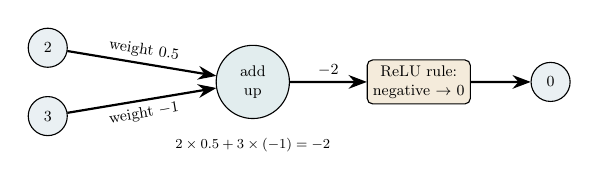
\begin{tikzpicture}[>=Stealth,every node/.style={font=\small},scale=0.62,transform shape]
\node[circle,draw,minimum size=8mm,fill=mist] (x1) at (0,1.0) {2};
\node[circle,draw,minimum size=8mm,fill=mist] (x2) at (0,-0.4) {3};
\node[circle,draw,minimum size=15mm,fill=teal!12,align=center] (s) at (4.2,0.3) {add\\up};
\node[draw,rounded corners=2pt,minimum height=8mm,fill=amber!15,align=center] (r) at (7.6,0.3) {ReLU rule:\\negative $\to$ 0};
\node[circle,draw,minimum size=8mm,fill=mist] (o) at (10.3,0.3) {0};
\draw[->,thick] (x1) -- node[above,sloped] {weight 0.5} (s);
\draw[->,thick] (x2) -- node[below,sloped] {weight $-1$} (s);
\draw[->,thick] (s) -- node[above] {$-2$} (r);
\draw[->,thick] (r) -- (o);
\node[font=\footnotesize] at (4.2,-1.0) {$2\times0.5 + 3\times(-1) = -2$};
\end{tikzpicture}
\caption{One neuron with made-up numbers. The sum $-2$ is negative, so ReLU turns it into 0.}
\end{figure}

\paragraph{The learning loop.} Weights start random. Then the network repeats: \textbf{guess}, \textbf{measure} how wrong (the loss), \textbf{nudge} every weight a little. The \term{loss} is the \term{mean squared error}: square each mistake and average (squaring stops $-0.1$ and $+0.1$ cancelling and punishes big mistakes more). To know which way to nudge, the network uses the \term{gradient}, the slope of the mistake: like standing on a foggy hill, feeling which way the ground slopes and stepping downhill. The step size is the \term{learning rate}, the method that decides each step is the \term{optimiser}. \term{Adam} is a popular optimiser that adapts its step size, and we used it throughout with learning rate 0.001. The network nudges after a small group of examples, a \term{batch} (16 in Colab, 1 on the laptop). One trip through all training examples is an \term{epoch} (we call it a pass).

\paragraph{Overfitting and early stopping.} A network can memorise its practice examples and fail on anything new. This is \term{overfitting}. We split each flood in time order: training (first 70\%, learned from), validation (15\%, checked during training) and test (last 15\%, used only at the end). A never-seen flood is an even harder exam. The sign of overfitting is practice error falling while validation error rises, and \term{early stopping} stops when validation stops improving and keeps the best version (used in Part 1). We meet a real case in Chapter~\ref{ch:res1}.

Models are written in \term{Python} with \term{TensorFlow} and \term{Keras}. A \term{GPU} does the many tiny calculations much faster than a \term{CPU}. Part 1 ran on a Colab GPU and Part 2 on one laptop CPU.

% =========================================================== CHAPTER 5
\section{Teaching a network to look at maps: the CNN}\label{ch:cnn}

A \term{convolutional neural network} (\term{CNN}) uses a small window called a \term{filter} (or \term{kernel}), commonly $3\times3$. We lay it over one spot, multiply the 9 numbers under it by 9 weights and add them: one number saying ``how much does this spot look like my pattern?'' Then we slide it one step (the \term{stride} is 1) until the map is covered, which gives a \term{feature map}. Adding a border of zeros (\term{padding}) keeps the map the same size. The \textbf{same filter is used everywhere}, so the parameter count stays small.

\begin{figure}[!htbp]
\centering
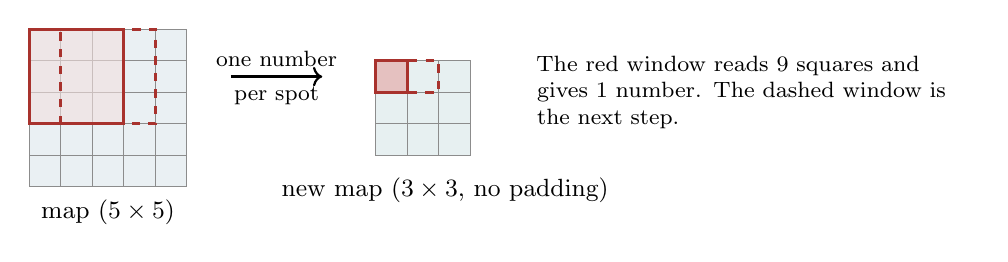
\begin{tikzpicture}[x=4mm,y=4mm,every node/.style={font=\small}]
\foreach \i in {1,...,5}{\foreach \j in {1,...,5}{\draw[black!45,fill=mist] (\i,\j) rectangle ++(1,1);}}
\draw[brick,very thick,fill=brick!15,fill opacity=0.6] (1,3) rectangle (4,6);
\draw[brick,very thick,dashed] (2,3) rectangle (5,6);
\node at (3.5,0.2) {map ($5\times5$)};
\draw[->,thick] (7.4,4.5) -- node[above,font=\footnotesize] {one number} node[below,font=\footnotesize] {per spot} (10.3,4.5);
\foreach \i in {1,...,3}{\foreach \j in {1,...,3}{\draw[black!45,fill=teal!10] (\i+11,\j+1) rectangle ++(1,1);}}
\draw[brick,very thick,fill=brick!30] (12,4) rectangle ++(1,1);
\draw[brick,very thick,dashed] (13,4) rectangle ++(1,1);
\node at (14.2,0.9) {new map ($3\times3$, no padding)};
\node[align=left,font=\footnotesize,text width=5.5cm] at (24,4) {The red window reads 9 squares and gives 1 number. The dashed window is the next step.};
\end{tikzpicture}
\caption{A filter slides over the map. Every spot gets one number.}
\end{figure}

One filter finds one pattern, so a layer uses many (for example 16), giving 16 feature maps that are the 16 \emph{channels} the next layer reads. A second convolution layer combines the simple patterns of the first (edges, slopes) into bigger ones such as a river bend, and each square sees a larger area. After each filter we apply ReLU. (Pooling is not used.) \textbf{Real count:} the first layer has 16 filters of $3\times3$ reading 3 channels, so $3\times3\times3=27$ weights plus 1 bias is 28 per filter and $16\times28=\mathbf{448}$ parameters. The second reads 16 channels: $3\times3\times16+1=145$ per filter and $16\times145=\mathbf{2{,}320}$.

% =========================================================== CHAPTER 6
\section{Teaching a network to remember: LSTM and ConvLSTM}\label{ch:lstm}

One flood map cannot tell you whether the water is rising, you need the map before it. An \term{LSTM} (\emph{long short-term memory}) reads one step at a time and keeps a memory, like a student with a notebook who at each step does three things: \textbf{forget} (erase what no longer matters), \textbf{write} (add what is useful) and \textbf{read} (look in the notebook to answer). Small dials called \term{gates} (forget, input, output) do these jobs, and the network learns how far to turn each. A normal LSTM keeps its memory as a short list of numbers. Ours must say something about \emph{each place}, so we use a \term{ConvLSTM}: its memory is a map and its gates use sliding filters like the CNN, so each square is updated using its neighbours too.

\begin{figure}[!htbp]
\centering
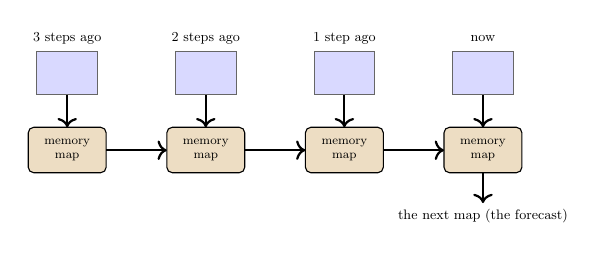
\begin{tikzpicture}[every node/.style={font=\small},scale=0.55,transform shape]
\foreach \i/\l in {0/{3 steps ago},3.2/{2 steps ago},6.4/{1 step ago},9.6/{now}}{
  \draw[fill=blue!15,draw=black!60] (\i,3) rectangle ++(1.4,1.0);
  \node at (\i+0.7,4.3) {\l};
  \draw[->,thick] (\i+0.7,3) -- (\i+0.7,2.25);
  \draw[fill=amber!25,rounded corners=2pt] (\i-0.2,1.2) rectangle ++(1.8,1.05);
  \node[align=center,font=\footnotesize] at (\i+0.7,1.72) {memory\\map};
}
\foreach \i in {0,3.2,6.4}{\draw[->,thick] (\i+1.6,1.72) -- (\i+3.0,1.72);}
\draw[->,thick] (10.3,1.2) -- (10.3,0.5) node[below,align=center,font=\small] {the next map (the forecast)};
\end{tikzpicture}
\caption{A ConvLSTM reads the maps in order and updates a memory that is itself a map.}
\end{figure}

Our ConvLSTM has 32 filters, and 55,424 of the 62,833 parameters live here. The big question of the project is: \textbf{does the memory actually help, or is a simpler method just as good?}

% =========================================================== CHAPTER 7
\section{The data: four floods}\label{ch:data}

\term{FloodCastBench} (Xu and co-authors, \emph{Scientific Data}, 2025) re-created four real floods in a physics simulator using real \textbf{ground height} (FABDEM), \textbf{land cover} and satellite \textbf{rain} (GPM-IMERG). Depth is given every 5 minutes, rain every 30. The maps are \textbf{simulated}, so our network learns to imitate the simulator, not real flooding.

\begin{table}[!htbp]
\centering\small
\caption{The four floods. ``Maps'' is the number of depth maps we keep, one every 30 minutes.}
\begin{tabularx}{\linewidth}{|>{\bfseries}l|Y|l|l|l|l|Y|}
\hline
\rowcolor{black!12} \hd{Flood} & \hd{Dates} & \hd{Square} & \hd{Map size} & \hd{Length} & \hd{Maps} & \hd{Our role}\\ \hline
Australia & 20 Feb to 2 Mar 2022 & 30 m & 1073 $\times$ 1073 & 10 days & 481 & Training\\ \hline
UK & 4 to 7 Dec 2015 & 30 m & 170 $\times$ 275 & 3 days & 145 & Never-seen test\\ \hline
Pakistan & 18 to 31 Aug 2022 & 480 m & 810 $\times$ 441 & 14 days & 673 & Training\\ \hline
Mozambique & 14 to 20 Mar 2019 & 480 m & 151 $\times$ 138 & 6 days & 289 & Never-seen test\\ \hline
\end{tabularx}
\end{table}

Australia and the UK also come at 60 m (used by the laptop study), made by resizing the 30 m results. Two pairs: learn from \textbf{Australia}, test on the \textbf{UK}, and learn from \textbf{Pakistan}, test on \textbf{Mozambique}.

\textbf{Getting the data ready.} (1) One map every 30 minutes. (2) One common grid: two independent checks (rivers of the land cover map and valleys of the ground height map against the water) agreed within about one square, then small squares were averaged into big ones. (3) Rain timing: rain file $j$ holds the rain in the 30 minutes \emph{after} depth map $j$, and on rainy steps the measured rise was 0.494 to 0.502 times the file value in all four floods, as expected for half an hour. (4) Three rain settings: \textbf{causal} (only past rain), \textbf{hybrid} (the original input, with up to 30 minutes of rain not yet fallen) and \textbf{forced} (the next five rain maps also given). (5) Local ground height: the height of a square minus the average around it (15 $\times$ 15 in Colab, the 128 $\times$ 128 patch on the laptop), because water flows by height differences. (6) \term{Tiles} (patches) of 64 $\times$ 64 in Colab and 128 $\times$ 128 on the laptop, because a million squares is too much in one piece. A trained network can then run on a whole map.

% =========================================================== CHAPTER 8
\section{The task and how we keep score}\label{ch:score}

\textbf{Part 1:} four depth maps 30 minutes apart plus rain and local height in, \textbf{one} map 30 minutes later out. \textbf{Part 2:} five maps in, the next five out (up to 2.5 hours) in one go.

\textbf{The simple forecasts we compare with.} \emph{Copy the last map} (persistence, skill 0 by definition), the \emph{trend forecast}, a \emph{linear model} of the depth history (fitted weighted sum), a \emph{lookup table} (average answer for each pair of current depth and last change) and a \emph{per-pixel MLP} (a tiny network looking at one square). The last three are Part 2 only. With $d_t$ the depth now and $d_{t-1}$ 30 minutes ago,
\[ \text{trend forecast} = \max\bigl(0,\; d_t + \beta\,(d_t - d_{t-1})\bigr). \]
Take the depth now, add a fraction $\beta$ of the last change, never go below zero. $\beta$ is fitted by least squares on the training part of the training flood only: \textbf{0.921} for 30 m and \textbf{0.948} for 480 m, a little below 1 so the change is continued but slightly slowed.

\textbf{The skill score.} Error is the average of squared mistakes over all squares, and
\[ \text{skill} = 1 - \frac{\text{error of the forecast}}{\text{error of copying the last map}}. \]
Skill 1 is perfect, 0 is no better than copying, below 0 is worse, and 0.9 removes 90\% of copying's error.

\textbf{Worked example.} Five squares: depth 30 minutes ago 0, 0.1, 0.4, 0.8, 1.0, now 0, 0.2, 0.5, 1.0, 1.0, what really happens 0, 0.3, 0.6, 1.2, 1.0. \emph{Copying} has mistakes 0, 0.1, 0.1, 0.2, 0 and squares adding to \textbf{0.06}. The \emph{trend} with $\beta=0.9$ gives 0, 0.29, 0.59, 1.18, 1.0, mistakes 0, 0.01, 0.01, 0.02, 0, squares adding to \textbf{0.0006}, so skill $=1-0.0006/0.06=0.99$. A \emph{bad model} giving 0, 0.5, 0.8, 1.1, 1.1 has squares adding to 0.10 and skill $\approx-0.67$, worse than copying (as Model A in late Australia, $-1.449$).

\fig{how_we_score.png}{0.45}{The skill score scale. \textbf{Say this:} 0 is copying the last map, 1 is perfect, negative is worse than copying.}

\textbf{Typical error in cm} (root mean square error) for copying the last map over the whole map: \textbf{0.112 cm (Australia, last 15\%), 0.520 (UK), 0.103 (Pakistan, last 15\%) and 0.548 (Mozambique)}. These tiny numbers are why copying is such a strong opponent.

\begin{carefulbox}
Skill in Colab and on the laptop is \textbf{not comparable}: Colab scores whole maps 30 minutes ahead, the laptop scores patches containing water from 30 minutes to 2.5 hours.
\end{carefulbox}

% =========================================================== CHAPTER 9
\section{How we tested fairly}\label{ch:test}

\textbf{Part 1.} One model per map size, trained on one flood in time order (70/15/15 as in Chapter~\ref{ch:nn}). Two tests: the \textbf{last 15\% of the training flood} and the harder \textbf{whole never-seen flood}.

\textbf{Part 2.} Three experiments named by map size: \textbf{E60} (Australia to UK, 60 m), \textbf{E30} (same at 30 m) and \textbf{E480} (Pakistan to Mozambique). Each has \textbf{three folds}, each holding out a different third of the training region's tiles (a second test, ``held-out tiles''). Every Part 2 number is the \textbf{mean of three folds}. Every model got the same fixed recipe: Adam, peak learning rate 0.001, 200-step warm-up then cosine decay, gradient clipping at 1.0, loss equal to squared error divided by the squared error of copying, batch 1, 30 passes and 300 training windows (a window is five maps in a row cut from a patch).

\textbf{Noise and intervals.} A \term{seed} fixes a network's random start. The spread between seeds is \textbf{0.006 to 0.010 in skill}, so we treat differences below about \textbf{0.02} as noise. A 95\% interval (from redrawing the test examples with replacement many times) that does not contain 0 means the difference is probably real.

\textbf{Hypotheses.} Before the final runs we wrote six: \textbf{H1} networks beat copying, \textbf{H2} they beat the best linear baseline, \textbf{H3} depth history matters, \textbf{H4} recurrence (LSTM memory) matters, \textbf{H5} more rain information helps, \textbf{H6} a stricter test gives a similar score. With extra runs this made about \textbf{310 training runs}.

\textbf{Ablations} take away one input at test time and see how far the score falls: ``rain removed'' and ``terrain removed'' set it to zero, ``history frozen'' replaces every earlier map with the last one, ``history shuffled'' puts the earlier maps in the wrong order. If the score hardly changes, the model did not use that input.

% =========================================================== CHAPTER 10
\section{Part 1: building the forecaster}\label{ch:build}

\begin{enumerate}
\item \textbf{Input:} four maps 30 minutes apart, three channels each (depth, rain, local ground height).
\item \textbf{Two CNN layers} (3 $\times$ 3, 16 filters) on each map: water edges, slopes, rain patches.
\item \textbf{The ConvLSTM} (3 $\times$ 3, 32 filters) reads the four maps in order and keeps a memory map.
\item \textbf{A small decoder} (one CNN layer and a last $1\times1$ layer) turns the memory into the \emph{predicted change in depth}.
\end{enumerate}
\fig{model_diagram.png}{0.5}{The forecaster in five boxes. The dark box is the memory (ConvLSTM). \textbf{Say this:} maps go through two CNN layers, the ConvLSTM remembers the four steps, and a small decoder draws the change.}

\textbf{Why predict the change, and start at zero?} Most of the map hardly changes in 30 minutes, so the network predicts only the change, added to a starting forecast. The last layer \textbf{starts at zero}, so before training the output is exactly the starting forecast. A final ReLU keeps depth from going below zero. Every convolution pads, so the map stays 64 $\times$ 64.

\begin{table}[!htbp]
\centering\small
\caption{Every layer of Model A for a 64 $\times$ 64 tile.}
\begin{tabularx}{\linewidth}{|Y|c|r|}
\hline
\rowcolor{black!12} \hd{Layer} & \hd{Output shape} & \hd{Parameters}\\ \hline
Input (depth, rain, local height) & 4 $\times$ 64 $\times$ 64 $\times$ 3 & 0\\ \hline
Convolution 3 $\times$ 3, 16 filters, ReLU (each map) & 4 $\times$ 64 $\times$ 64 $\times$ 16 & 448\\ \hline
Convolution 3 $\times$ 3, 16 filters, ReLU (each map) & 4 $\times$ 64 $\times$ 64 $\times$ 16 & 2,320\\ \hline
ConvLSTM 3 $\times$ 3, 32 filters & 64 $\times$ 64 $\times$ 32 & 55,424\\ \hline
Convolution 3 $\times$ 3, 16 filters, ReLU & 64 $\times$ 64 $\times$ 16 & 4,624\\ \hline
Convolution 1 $\times$ 1, 1 filter (starts at zero) & 64 $\times$ 64 $\times$ 1 & 17\\ \hline
Add to the starting forecast, then ReLU & 64 $\times$ 64 $\times$ 1 & 0\\ \hline
\textbf{Total} & & \textbf{62,833}\\ \hline
\end{tabularx}
\end{table}

\textbf{Model A and Model B} have \emph{exactly the same layers} and differ in the last step. \textbf{Model A} starts from the last map and adds the predicted change in metres. \textbf{Model B} starts from the trend forecast and adds a small correction in centimetres. We built B after A beat copying but the trend forecast was far better.

\textbf{Training.} 4,000 random 64 $\times$ 64 tiles for learning and 600 for validation, Adam at constant learning rate 0.001, batch 16, up to 20 passes, early stopping after 4 passes without improvement (best weights kept), seed 42, mean squared error loss, one model per map size and version, on a Colab GPU.

% =========================================================== CHAPTER 11
\section{Part 1 results: the surprise}\label{ch:res1}

\begin{table}[!htbp]
\centering\small
\caption{Skill against copying the last map, whole maps, 30 minutes ahead (single runs). ``Rule'' is the water-balance rule below.}\label{tab:p1}
\begin{tabularx}{\linewidth}{|>{\bfseries}p{3.5cm}|Y|Y|Y|Y|Y|Y|}
\hline
\rowcolor{black!12} \hd{Test} & \hd{Trend} & \hd{Copy + rule} & \hd{A} & \hd{A + rule} & \hd{B} & \hd{B + rule}\\ \hline
Australia, last 15\% & 0.990 & 0.000 & $-1.449$ & $-0.710$ & 0.989 & 0.989\\ \hline
UK, never-seen flood & 0.947 & 0.053 & 0.305 & 0.320 & 0.948 & 0.949\\ \hline
Pakistan, last 15\% & 0.908 & 0.142 & 0.345 & 0.404 & 0.908 & 0.901\\ \hline
Mozambique, never-seen flood & 0.942 & 0.051 & 0.150 & 0.172 & 0.943 & 0.941\\ \hline
\end{tabularx}
\end{table}

Model A beat copying in three of four tests (0.305, 0.345, 0.150), but the trend forecast with no network scores 0.908 to 0.990, far ahead of Model A in every test. In late Australia Model A scored $-1.449$. \textbf{Model B matches the trend within 0.001 in every test but does not beat it.} A network that beats ``copy'' can still be bad: ask whether it beats the \emph{best simple forecast}.

\fig{trend_vs_models.png}{0.5}{Skill of the trend forecast (no network), Model A and Model B in the four tests.}

\textbf{What went wrong in late Australia.} There the water hardly moves and copying is wrong by only about a millimetre, so a model adding even a little water in the wrong place is worse than copying. Our first guess, that the model had only seen water rising, was \textbf{wrong}: in 73 of 331 training steps the average depth fell, and the trend number fitted on them scores 0.990 on that last part. The error maps show a faint excess of water over most of the map at the start of this part, and strong errors for A along rivers and heavy rain, but almost none for B. We think A added a little water almost everywhere, but we did \textbf{not} measure this further.

\textbf{Why B could not do better.} Training lowered B's validation error only about 1\% (30 m) and 5\% (480 m). After the trend only \textbf{1\% in Australia, 5\% in the UK, 9\% in Pakistan and 6\% in Mozambique} of copying's error is left. For the 30 m Model A the validation error was lowest after the second pass and then rose while practice error kept falling: the overfitting of Chapter~\ref{ch:nn}.

\begin{carefulbox}
We changed \emph{two} things in Model B at once (starting point and unit of the correction), so we cannot say which made the difference.
\end{carefulbox}

\textbf{The water-balance rule}\label{sec:rule}. Almost all the rain stays on the ground, so the average rise of the water in 30 minutes should equal rain (mm per hour) times 0.5 hours (4 mm per hour should raise the average depth by 2 mm). The \term{water-balance rule} shifts the forecast so its total change matches the last 30 minutes of rain. The data obey it closely (ratio 0.999 Australia, 0.946 UK, 1.028 Pakistan, 1.045 Mozambique, since water leaves at the map edge in three floods and the Indus flows in at Pakistan's edge). The rule \textbf{helped Model A in every test}, halving the Australian failure ($-1.449$ to $-0.710$), but changed Model B by only $-0.007$ to $+0.001$. It patched A's weakness and adds no skill to a good forecast.

% =========================================================== CHAPTER 12
\section{Part 2: the big laptop study}\label{ch:p2set}

Part 1 left open: which parts of a CNN-LSTM matter? We ran about \textbf{310 training runs} on one laptop, up to 2.5 hours ahead. The models: four fitted baselines (linear model of depth history, the same with rain, state and trend, two-feature lookup table, per-pixel MLP), the \textbf{original CNN-LSTM} (about 4.5 million parameters), a CNN with a 1 $\times$ 1 kernel (one square only), the \textbf{local CNN} (one 5 $\times$ 5 convolution of 16 filters and a 1 $\times$ 1, no memory, 4,101 parameters), a CNN with an 11 $\times$ 11 kernel, the \textbf{small ConvLSTM} (8 filters, 4,741 parameters) and a heavy ConvLSTM (652,918, about 140 times larger).

\textbf{A worrying design in the original CNN-LSTM.} About 93\% of its parameters sit in two dense layers of $16{,}384\times128$ weights, and it squeezes every frame through just \textbf{128 numbers} before the LSTM, like describing a photo over the phone: you can say ``mostly blue'' but not that one pebble moved a millimetre. Its depth input was also divided by 5 m, so a millimetre becomes tiny. We think these choices explain its poor score but did not test this directly.

% =========================================================== CHAPTER 13
\section{Part 2 results: what really matters}\label{ch:res2}

Scores are skill on a \textbf{never-seen flood}, mean of three folds, hybrid rain, five maps from 30 minutes to 2.5 hours.

\begin{table}[!htbp]
\centering\small
\caption{Skill on the never-seen flood against copying. Seed noise is about 0.01.}
\begin{tabularx}{\linewidth}{|Y|c|c|c|}
\hline
\rowcolor{black!12} \hd{Forecast} & \hd{E60 (UK)} & \hd{E30 (UK)} & \hd{E480 (Moz.)}\\ \hline
Lookup table (two features) & 0.786 & 0.763 & 0.737\\ \hline
Linear model of the depth history & 0.818 & 0.798 & 0.790\\ \hline
Per-pixel MLP & 0.846 & 0.854 & 0.829\\ \hline
Original CNN-LSTM & 0.187 & 0.188 & 0.061\\ \hline
CNN 1 $\times$ 1 kernel / local CNN 5 $\times$ 5 / CNN 11 $\times$ 11 & 0.848 / 0.841 / 0.841 & 0.835 / 0.830 / 0.831 & 0.818 / 0.807 / 0.793\\ \hline
Small ConvLSTM & 0.866 & 0.840 & 0.811\\ \hline
Heavy ConvLSTM & 0.840 & not run & 0.802\\ \hline
\end{tabularx}
\end{table}

Three findings. (1) \textbf{A simple formula does most of the work.} The linear model scores 0.79 to 0.82 and the best networks 0.81 to 0.87, so they add only about 0.01 to 0.05. (2) \textbf{Neighbours and size do not help.} Kernels of size 1, 5 and 11 are within 0.025 of each other and a network 140 times larger gains nothing. (3) \textbf{The original CNN-LSTM is far behind} at 0.06 to 0.19.

\textbf{What the models used.} Freezing or shuffling the history leaves the original CNN-LSTM at 0.187, so it \textbf{ignores the history}, and removing rain drops it to 0.003, so it works almost only from rain. For the other networks \textbf{history frozen} takes skill to about zero and \textbf{history shuffled} to $-2.6$ to $-3.7$, so they depend on the history and its order, while rain removed costs 0.01 to 0.02 and terrain removed 0.006 or less. A local CNN \emph{trained} without depth history falls from 0.84, 0.83 and 0.81 to \textbf{0.17, 0.16 and 0.09}. The rain setting matters a little: for the local CNN causal, hybrid and forced rain give 0.822, 0.841, 0.866 (E60), 0.805, 0.830, 0.851 (E30) and 0.794, 0.807, 0.834 (E480).

\textbf{Does the LSTM memory help?} Not when compared fairly. At 30 passes the small ConvLSTM led the local CNN on UK 60 m by $+0.025$ (95\% interval $+0.004$ to $+0.043$) and was level on Mozambique. But the plain CNN was undertrained: with 90 passes for both, the difference was $+0.004$ ($-0.021$ to $+0.027$) on the UK and $-0.014$ ($-0.029$ to $+0.006$) on Mozambique, inside the $\pm0.03$ band fixed in advance as ``equivalent''. The ConvLSTM looked better in two places (it loses skill more slowly further ahead, and it is steadier in the strict test below), but we did not test that recurrence is the reason.

\fig{what_models_use.png}{0.4}{What the networks use. \textbf{Say this:} taking away the depth history ruins the forecast, taking away rain or terrain hardly matters.}

\textbf{Tuning.} A larger batch (8) with learning rate $3\times10^{-3}$ lowered scores by 0.008 to 0.026. Longer training (90 passes) helped the plain CNN by 0.008 to 0.024 and the ConvLSTM almost nothing. Differences below about 0.02 cannot be resolved.

\textbf{The strict test.} Hiding a whole block of time, including the start of a flood, the plain CNN on hidden Pakistan tiles fell from skill 0.430 to \textbf{$-6.56$}. Six of 480 windows, all at the very start of the flood, carried \textbf{98\% of the error}. The ConvLSTM stayed at \textbf{0.742} and the lookup table at 0.66. A model that has not seen the start of a flood should not be trusted on one.

\textbf{Scorecard of the six hypotheses} (16 cells in all). H1 held in 13 of 16. H2 held in 15 of 16 (gain 0.02 or more in 8, within noise in 7, linear better by 0.046 in 1). H3 held in all three experiments (a loss of 0.67 to 0.72 without history). H4 mixed: ahead at 30 passes, not supported at 90. H5 held for the local CNN, not for the ConvLSTM. H6 held in only 2 of 5 cells.

% =========================================================== CHAPTER 14
\section{A mistake we found, and how we fixed it}\label{ch:bug}

The laptop linear baselines were \term{ridge regressions}: weighted sums fitted by least squares with a penalty on big weights. Our inputs were in \emph{metres}, and 30-minute depth changes are tiny (about 0.003), so such an input needs a \textbf{big} weight, which the penalty punishes. The penalty squeezed the history weights almost to zero, so two linear baselines \textbf{could not use the depth history} and looked far weaker than they are, which made the networks look better than they should.

\textbf{Aman found it on 10 October 2026.} Re-running the old code reproduced the old numbers exactly in all 9 combinations. We then \textbf{standardised every input} (same spread) before fitting, and a fit with almost no penalty matched it within 0.001.

\begin{table}[!htbp]
\centering\small
\caption{Skill of the two affected linear baselines (never-seen flood, hybrid rain) before and after the fix.}
\begin{tabularx}{\linewidth}{|>{\bfseries}p{5.6cm}|Y|Y|Y|}
\hline
\rowcolor{black!12} \hd{Linear baseline} & \hd{E60} & \hd{E30} & \hd{E480}\\ \hline
Depth history: before / after & 0.323 / 0.818 & 0.345 / 0.798 & 0.151 / 0.790\\ \hline
With rain, state and trend: before / after & 0.345 / 0.820 & 0.359 / 0.797 & 0.182 / 0.793\\ \hline
\end{tabularx}
\end{table}

Our claim that the forecast is a \emph{non-linear} function of the depth history is \textbf{not supported}, and H2 went from 16 of 16 to \textbf{15 of 16}. \textbf{Not affected:} the Colab results, H1, H3 to H6, the lookup table, MLP, networks, ablations and tuning. The corrected numbers are those in the final report. Lesson: a weak baseline flatters a model, so check that baselines are strong and fair.

% =========================================================== CHAPTER 15
\section{Rating the flood: capsule network and written rules}\label{ch:capsule}

We rate each 64 $\times$ 64 tile as \textbf{none, minor, moderate or severe}. The \term{label} is the share of the tile's \emph{normally dry land} under more than 30 cm of water: none below 5\%, minor 5\% to 15\%, moderate 15\% to 30\%, severe 30\% or more. (The earlier laptop label, the single deepest square, let one deep spot decide a whole patch and failed outside Australia at 30 m.) In Pakistan 698 of the 1,000 test tiles are severe, in the UK none.

\textbf{Capsule network.} In an ordinary network every neuron outputs \emph{one number}. A capsule outputs a small \emph{list} (a vector): its \textbf{length} says how sure it is that something is there and its \textbf{direction} gives details. Capsules in one layer \emph{vote} for capsules in the next, and votes that agree with the others get more weight, \term{routing by agreement} (like eight friends saying ``robin'' and two ``crow'': you trust the eight). Our code repeats it three times. Our capsule head takes the frozen ConvLSTM memory map, shrinks it with three convolutions, forms \textbf{256 primary capsules} (8 numbers each), and routes them through \textbf{three rounds} to \textbf{four class capsules} (16 numbers each), the longest being the answer. The \term{margin loss} pushes the correct capsule's length above 0.9 and the others below 0.1.

As a control, a plain dense layer on Australia at 30 m (earlier label) scored 60.2\% against the capsule's 67.8\% without augmentation, but 79.8\% against 80.3\% with augmentation (rotating and flipping patches, 8 versions), a gap of $+0.005$ with an interval around zero. A trivial rule on the last observed map scored \textbf{97.4\%}, so neither network beat a simple threshold.

\begin{table}[!htbp]
\centering\small
\caption{Severity accuracy on 1,000 test tiles per flood (Colab notebook, new label).}\label{tab:caps}
\begin{tabularx}{\linewidth}{|>{\bfseries}p{3.6cm}|Y|Y|Y|}
\hline
\rowcolor{black!12} \hd{Test flood} & \hd{Capsule alone} & \hd{Capsule + rules} & \hd{Class of the forecast map alone}\\ \hline
Australia (30 m) & 60.9\% & 67.9\% & 99.8\%\\ \hline
UK (30 m) & 50.0\% & 56.1\% & 99.1\%\\ \hline
Pakistan (480 m) & 87.4\% & 89.1\% & 99.9\%\\ \hline
Mozambique (480 m) & 63.5\% & 70.7\% & 99.5\%\\ \hline
\end{tabularx}
\end{table}

The last column is almost perfect because the rating in 30 minutes is nearly the rating now. \textbf{Pakistan's 87.4\% is not as good as it looks}, since always answering ``severe'' is right 69.8\% of the time, and 30 m and 480 m accuracies should not be compared (a tile covers about 2 km at 30 m, 30 km at 480 m). A \term{confusion matrix} is a table of right and wrong answers, with correct ones on the diagonal.

\textbf{NeuroSymbolic AI} joins a neural network (``neuro'') with written rules people can read (``symbolic''), so they can check each other. Our physics rule checks the forecast (Chapter~\ref{ch:res1}) and three severity rules check the capsule's answer: \textbf{R1} if less than 1\% of the land is flooded now and in the forecast, the rating is ``none''. \textbf{R2} if the forecast is not less flooded than now and more than 1 mm per hour of rain fell in the last hour, the rating may not fall below the current level. \textbf{R3} if the capsule's and the forecast map's ratings are more than one class apart, use the forecast map's. Every decision comes with a written reason. Of 1,000 tiles the rules changed R1/R2/R3: Australia 49/0/21, UK 0/40/21, Pakistan 0/7/10, Mozambique 134/42/0, and accuracy rose in all four floods (table above). In the laptop study the rule layer even lowered accuracy (80.3\% to 74.1\%), and its rules and labels are different, so the two cannot be compared.

% =========================================================== CHAPTER 16
\section{Looking inside: Grad-CAM and explainable AI}\label{ch:gradcam}

A network is a \emph{black box}, and \term{explainable AI} helps people see what a model is doing. \term{Grad-CAM} uses the \emph{gradient} of Chapter~\ref{ch:nn}, but about the \emph{answer}: if this part of the memory were turned up a little, how much would the answer move? The ConvLSTM keeps 32 memory maps, each gets a weight from how much it moves the answer, and we add them with those weights, keep the positive part and paint it on the picture. Bright places mattered. For the forecaster the quantity explained is the \textbf{total predicted depth}, for the capsule network the \textbf{length of the chosen class capsule}. In Australia and the UK the bright areas \textbf{follow river channels and flood edges}, in Pakistan large blocks (we think heavy rain) and in Mozambique drainage lines.

\textbf{Are the heat maps honest?} In the laptop study a \term{deletion test} removed the 10\% of cells with the highest heat. For the depth forecast this changed the forecast more than random cells in \textbf{84\% to 92\%} of windows, so it passed. For the severity class the heat maps were weak: the top cells beat the controls in only 55\% of windows, and maps of two seeds agreed with a rank correlation of only \textbf{0.17}. We treat the capsule heat maps as illustrations, \textbf{not proof}.

\begin{figure}[!htbp]
\centering
\begin{minipage}[t]{0.47\linewidth}\centering
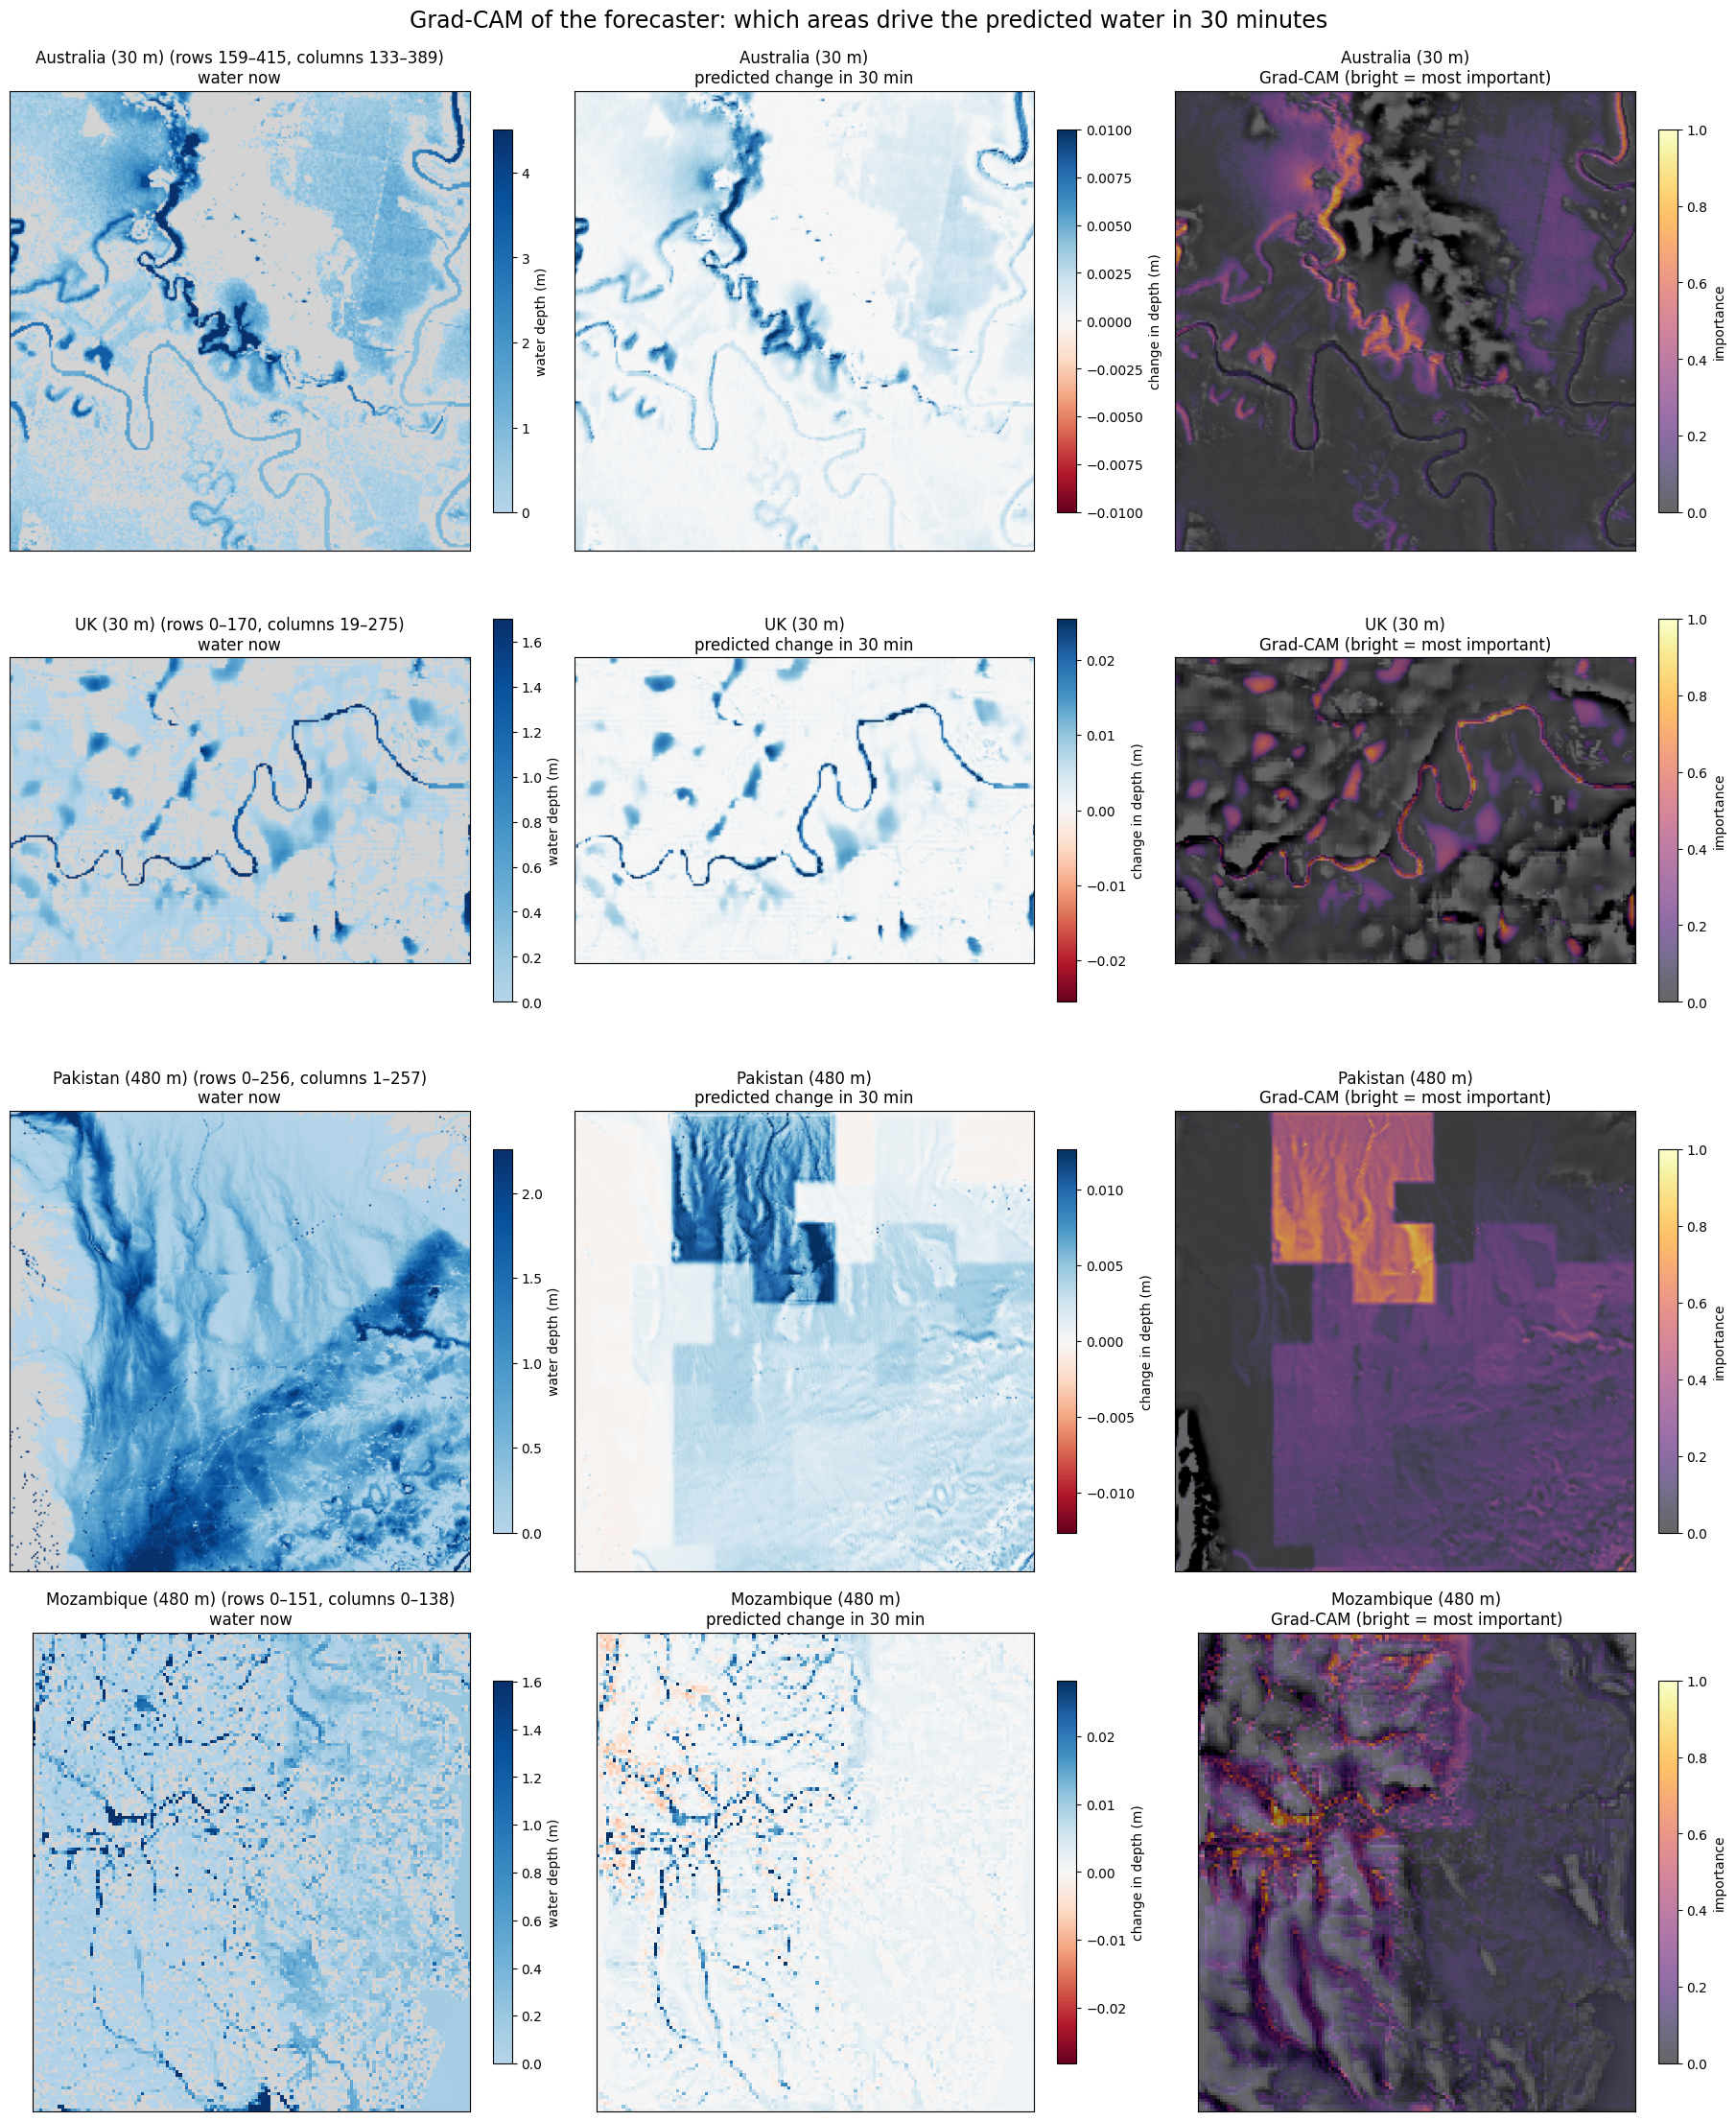
\includegraphics[width=\linewidth]{img/grad_cam_forecaster.png}\captionof{figure}{Grad-CAM of the forecaster (Model A): water now, predicted change, heat map over local ground height. \textbf{Say this:} the bright places follow rivers and flood edges.}
\end{minipage}\hfill
\begin{minipage}[t]{0.47\linewidth}\centering
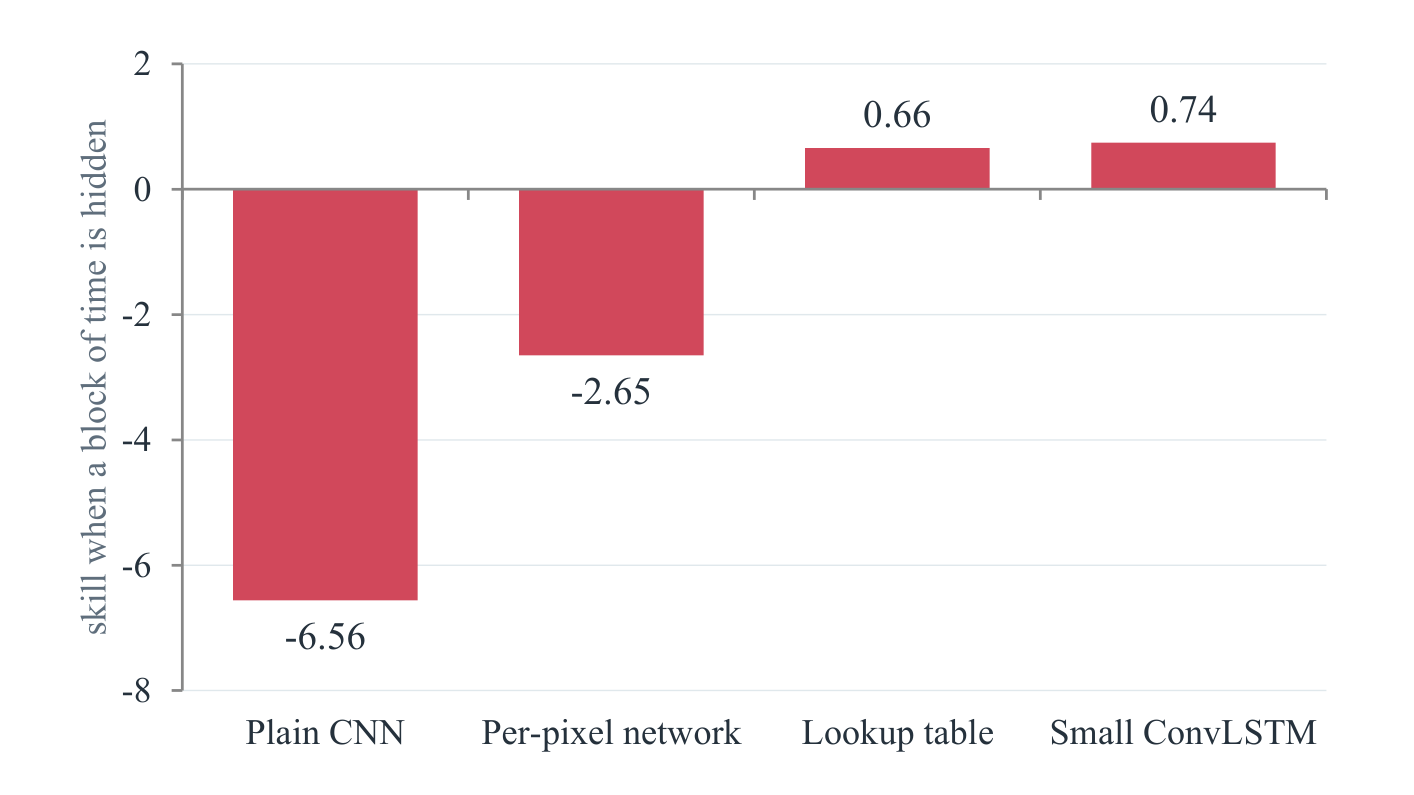
\includegraphics[width=\linewidth]{img/strict_split.png}\captionof{figure}{The strict test (start of a flood hidden). \textbf{Say this:} the plain CNN breaks down, the ConvLSTM and lookup table stay steady.}
\end{minipage}
\end{figure}

\textbf{Where each course keyword appears:} CNN (Chapters 5, 10), LSTM and ConvLSTM (6, 10, 13), capsule network (15), NeuroSymbolic AI (11, 15), explainable AI and Grad-CAM (16).

% =========================================================== CHAPTER 17
\section{Limits, lessons and what comes next}\label{ch:limits}

\textbf{What this study cannot tell you.} Only two independent test pairs (Australia to UK, Pakistan to Mozambique). The floods are simulated. Part 1 results are single runs. The two parts use different protocols and cannot be compared. The capsule network and Grad-CAM were built on Model A, not B. The LSTM memory is untested beyond 2.5 hours. A plain CNN can break completely at the start of a flood it never saw.

\textbf{Lessons.} (1) Compare every model with simple forecasts. (2) A weak baseline flatters a model. (3) Check your own explanations (we first thought Model A never saw draining water, and the data said no). (4) A bigger network is not automatically better. (5) Know your noise: differences below about 0.02 are not claimed. (6) Test on unseen places and hide a block of time too. (7) Write hypotheses down first, and say what you do not know.

\textbf{Next.} Forecast 6 to 24 hours by feeding forecasts back. Split Model B's two changes apart. Rebuild the capsule network and Grad-CAM on Model B. Repeat the Colab runs with several seeds.

\textbf{Conclusion.} We built a CNN-ConvLSTM forecaster for flood depth maps, added a capsule severity network, Grad-CAM and written rules, and tested them on later parts of the training floods and on floods from other countries. Model A beat the easiest reference and looked successful, a second simple reference was far better, and Model B matched it. The laptop study showed the depth history carries nearly all of the skill, and at equal training length the ConvLSTM was no more accurate than a plain CNN, though steadier when the start of a flood was hidden.

% =========================================================== KEY NUMBERS
\origsection{The key numbers on one page}\label{ch:nums}

Part 1 is the Colab notebook and Part 2 the laptop study. The four tests are always in the order Australia, UK, Pakistan, Mozambique.

\begin{table}[!htbp]
\centering\small
\caption{The numbers to remember.}
\begin{tabularx}{\linewidth}{|>{\bfseries}p{4.3cm}|Y|}
\hline
\rowcolor{black!12} \hd{What} & \hd{The number}\\ \hline
The floods & Four. Learn from Australia and Pakistan, test on the never-seen UK and Mozambique.\\ \hline
Square sizes & 30 m (Australia, UK) and 480 m (Pakistan, Mozambique).\\ \hline
Maps kept & One every 30 minutes: 481, 145, 673 and 289 maps.\\ \hline
Part 1 forecaster & 62,833 parameters. Four maps in, one map out, 30 minutes ahead.\\ \hline
Error of copying the last map & 0.112, 0.520, 0.103 and 0.548 cm.\\ \hline
Trend number $\beta$ & 0.921 for 30 m and 0.948 for 480 m.\\ \hline
Skill of the trend forecast & 0.990, 0.947, 0.908 and 0.942.\\ \hline
Skill of Model A & $-1.449$, 0.305, 0.345 and 0.150.\\ \hline
Skill of Model B & 0.989, 0.948, 0.908 and 0.943.\\ \hline
Error left after the trend & 1\%, 5\%, 9\% and 6\% of the error of copying.\\ \hline
Part 2 size & About 310 training runs. Five maps in, five out, up to 2.5 hours ahead.\\ \hline
Part 2 skill & Lookup table 0.74 to 0.79. Linear model 0.79 to 0.82. Best networks 0.81 to 0.87. Original CNN-LSTM 0.06 to 0.19.\\ \hline
Noise between seeds & 0.006 to 0.010, so treat differences below about 0.02 as noise.\\ \hline
A network 140 times larger & No gain (0.840 and 0.802).\\ \hline
Capsule network against a plain layer & 67.8\% against 60.2\%, but 80.3\% against 79.8\% with augmentation.\\ \hline
Capsule network with the rules (Part 1) & 67.9\%, 56.1\%, 89.1\% and 70.7\%.\\ \hline
Grad-CAM deletion test & 84\% to 92\% of windows for the depth forecast.\\ \hline
Strict test on hidden Pakistan tiles & Plain CNN 0.430 down to $-6.56$. ConvLSTM 0.742. Lookup table 0.66.\\ \hline
\end{tabularx}
\end{table}

% =========================================================== WHY THIS DESIGN (one-liners)
\section{Why this design? One-line answers for every choice in the model}\label{ch:design}

Mam will ask about the code and the theory behind it, for example ``why 16 filters?''. Each answer below is one sentence you can say aloud, with a short note in small print for when she asks more. Tags: \textbf{Notebook} means the notebook or report says it, \textbf{Evidence} means one of our own experiments shows it, \textbf{General} means it is the usual reason and we did not test it. We never ran an experiment that changes the number of filters or layers of Model A, so never say ``we tried 8 and 32''.

\begin{table}[!htbp]
\centering\small
\caption{Model A layer by layer for a 64 by 64 tile (Model B has the same layers). Parameters match the notebook's \cd{summary()}, total 62,833.}\label{tab:layers}
\begin{tabularx}{\linewidth}{|>{\ttfamily}p{2.2cm}|p{3.6cm}|p{2.5cm}|r|Y|}
\hline
\rowcolor{black!12} \hd{Name} & \hd{Keras call} & \hd{Output shape} & \hd{Params} & \hd{Job}\\ \hline
past\_maps & Input & 4, 64, 64, 3 & 0 & Four maps: depth, rain, local height.\\ \hline
cnn\_1 & TimeDistributed (Conv2D(16, 3, same, relu)) & 4, 64, 64, 16 & 448 & 16 simple patterns per map.\\ \hline
cnn\_2 & TimeDistributed (Conv2D(16, 3, same, relu)) & 4, 64, 64, 16 & 2,320 & Bigger shapes from the simple ones.\\ \hline
memory & ConvLSTM2D(32, 3, same) & 64, 64, 32 & 55,424 & Reads the 4 maps in order, keeps 32 memory maps.\\ \hline
decoder & Conv2D(16, 3, same, relu) & 64, 64, 16 & 4,624 & Memory to 16 working features.\\ \hline
depth\_change & Conv2D(1, 1), starts at zero & 64, 64, 1 & 17 & 16 features to one number: the change in depth.\\ \hline
add, next\_depth & Add, then ReLU & 64, 64, 1 & 0 & Last depth plus change, never below 0.\\ \hline
\end{tabularx}
\end{table}
\textbf{Counting parameters:} kernel height $\times$ width $\times$ input layers $\times$ filters, plus one bias per filter. \cd{cnn\_1}: $3\cdot3\cdot3\cdot16+16=448$. \cd{cnn\_2}: $3\cdot3\cdot16\cdot16+16=2{,}320$. \cd{decoder}: $3\cdot3\cdot32\cdot16+16=4{,}624$. \cd{depth\_change}: $16+1=17$. ConvLSTM: four parts (three gates and the candidate) over 16 input plus 32 memory layers, $4(3\cdot3\cdot48\cdot32+32)=55{,}424$, which is 88\% of the model.

\subsection{The layers}
\qq{Why a CNN and not a dense network?}{A flood is a picture, and a convolution looks at neighbouring squares with the same small detector everywhere.}{Evidence: the original laptop model squeezed each frame through a dense layer of 128 numbers and scored only 0.06 to 0.19, while local convolutional networks scored 0.81 to 0.87.}
\qq{Why 16 filters?}{It is a small standard size and each filter learns one pattern, but the notebook does not say why 16 was chosen and we did not tune it.}{General. Evidence: laptop networks of 4,101, 4,741 and 652,918 parameters all scored within about 0.03, so size was not the limit.}
\qq{Why a second convolution layer?}{A second 3 by 3 layer sees a 5 by 5 area, so it finds bigger shapes such as river bends with fewer weights than one 5 by 5 filter.}{General, we did not test removing it. Two 3 by 3 layers use 18 weights per channel pair against 25, and add one more ReLU bend.}
\qq{Why a 3 by 3 kernel?}{It is the smallest filter that sees a square and all eight neighbours, so it can see the direction of a slope.}{Evidence: kernels of 1, 5 and 11 scored within 0.025 in the laptop study, so neighbours add little.}
\qq{What does padding same do?}{It adds a border of zeros so the output stays 64 by 64, which is needed to add the change to the last depth map square by square.}{}
\qq{Why ReLU, and why none on the last convolution?}{ReLU zeroes negatives and gives the network the bend it needs, and the change in depth can be negative, so the last convolution has none.}{The final ReLU after the addition only keeps the depth from going below zero.}
\qq{What does TimeDistributed do?}{It runs the same convolution, with the same weights, on each of the four maps separately.}{Shape (4, 64, 64, 3) becomes (4, 64, 64, 16), and sharing weights is why \cd{cnn\_1} costs 448 and not $4\times448$.}
\qq{Why a ConvLSTM with 32 filters?}{We need to remember how the water moved over 1.5 hours, and a ConvLSTM keeps its memory as a map, using 32 memory layers.}{General for 32, not tuned. Evidence: an 8-filter ConvLSTM scored 0.866, 0.840, 0.811 in the laptop study, and one 140 times larger did not do better (these are not Models A and B).}
\qq{What does the ConvLSTM output?}{By default only the memory after the last of the four steps, shape (64, 64, 32), which is all we need for one forecast.}{}
\qq{Why a decoder layer and a final 1 by 1 convolution?}{The decoder turns the 32 memory maps into 16 features, and the 1 by 1 layer mixes them into one number per square, the predicted change, with 17 parameters.}{}
\qq{Why no pooling, dropout or batch normalisation?}{Pooling would shrink the map and we need an answer for every square, the model is small, and early stopping handles overfitting.}{We did not try dropout or batch normalisation.}
\qq{Why does the last layer start at zero?}{With zero weights the predicted change is zero, so before training the model exactly copies the last map.}{Notebook. In Model B the same trick starts it exactly at the trend forecast, and the notebook checks the difference is 0.0.}
\qq{Why predict the change and not the whole map?}{In 30 minutes most squares hardly change, so learning the small difference is much easier than redrawing the map.}{}

\subsection{Data and training}
\qq{Why 4 input maps?}{Four maps 30 minutes apart show the last 1.5 hours, enough to see whether the water is rising, falling or steady.}{It is the setting \cd{INPUT\_STEPS = 4}. We did not test other lengths in Part 1.}
\qq{Why 64 by 64 tiles, and why 4,000?}{The Australia map is 1073 by 1073, too big to train in one piece, and a network of small filters can run on a whole map afterwards.}{4,000 training, 600 checking, 1,000 test tiles. \cd{forecaster\_for\_whole\_map} copies the weights into a whole-map model.}
\qq{Why divide rain by 10 and use local ground height?}{Rain is scaled to a similar size as the other inputs, and water flows because of height differences to the neighbours, so we use height minus the 15 by 15 average.}{Notebook.}
\qq{Why mean squared error?}{Our skill score is built on squared error, so we train on what we are scored on, and big mistakes count more.}{Model B uses centimetres because, says the notebook, in metres the numbers are tiny.}
\qq{Why Adam, learning rate 0.001, batch 16, 20 epochs?}{They are the usual safe settings, Adam adapts its own step size, and 20 is only a ceiling because early stopping ends training sooner.}{General. Evidence: in the laptop study a bigger batch with a higher rate cost 0.008 to 0.026 and longer training gained up to 0.024, both near seed noise of about 0.01.}
\qq{How does early stopping work?}{\cd{EarlyStopping(patience=4, restore\_best\_weights=True)} stops after 4 epochs without improvement on the 600 checking tiles and restores the best weights.}{For the 30 m Model A the checking error was lowest after the second epoch, then rose: overfitting.}
\qq{Why a 70, 15, 15 split in time?}{Checking and test parts come after the training part, like a real forecast, and beta uses only the training part, so there is no leakage.}{}
\qq{Why two models, 30 m and 480 m?}{A 30 m and a 480 m square behave very differently, so we never mix them: Australia to UK, and Pakistan to Mozambique.}{}
\qq{Why not a Transformer or U-Net?}{Our project was a CNN with an LSTM memory, and the dataset's own benchmark has U-Net and FNO but no recurrent model.}{Evidence: a local CNN with no recurrence scored the same at equal training length ($+0.004$ and $-0.014$, inside the $\pm0.03$ band).}

\subsection{Trend forecast, Model B and the water rule}
\qq{How is beta found?}{It is the least-squares number, the sum of previous change times next change divided by the sum of previous change squared, giving 0.921 for 30 m and 0.948 for 480 m.}{That is \cd{top / bottom} in \cd{fit\_trend\_factor}. Below 1 means the change carries on but slows.}
\qq{What do Subtract and Rescaling do in Model B?}{Subtract gives the last change, Rescaling(beta) scales it, Add and ReLU make the trend forecast, and the network's output times 0.01 is added as a correction in centimetres.}{}
\qq{Why does Model B not beat the trend?}{At 30 minutes the trend already removes 91 to 99\% of copying's squared error, leaving only 1, 5, 9 and 6\%.}{If training does not lower the checking error the code keeps the plain trend (\cd{if best\_loss >= start\_loss}).}
\qq{How does the water-balance rule work?}{Average rise should equal rain times 0.5 hours, so the rule adds missing water to every square or removes extra water only from wet squares.}{It fixes the total only, the network still decides where the water goes.}

\subsection{Capsule network, Grad-CAM and the labels}
\qq{Why a capsule network?}{It was in our proposal, and a capsule's length says how sure the network is, which suits a severity rating.}{It did not beat a plain layer once we used augmentation, and the forecast map's own class is right 99\% of the time.}
\qq{Why is the ConvLSTM frozen in the capsule model?}{We reuse the forecaster's memory and train only the new layers, which is faster and needs fewer examples.}{General. It also lets one Grad-CAM function explain both models.}
\qq{Why strided convolutions and 256 primary capsules?}{Each stride-2 convolution halves the map (64, 32, 16, 8) and $8\times8\times4$ types gives 256 capsules of 8 numbers.}{The notebook gives no reason for the kernel sizes (5, 5, 3) or the count, general reasoning only.}
\qq{What does squash do?}{It shrinks a vector's length to between 0 and 1 and keeps its direction, so length can mean confidence.}{Formula in the code: $\frac{|v|^2}{1+|v|^2}\cdot\frac{v}{|v|}$.}
\qq{What is routing by agreement?}{Each small capsule votes for each class, votes that agree with the result get more weight next round, and the code repeats this 3 times.}{The vote weights are $256\times4\times16\times8=131{,}072$ numbers, with a softmax over the 4 classes.}
\qq{What is the margin loss?}{The true class capsule should be longer than 0.9 and the others shorter than 0.1, with the others weighted 0.5.}{Same constants as Sabour et al., not tuned by us. The notebook comment says class weights stop it answering None every time.}
\qq{Why Grad-CAM at the ConvLSTM memory?}{It is the last layer that is still a map and is shared by the forecaster and the capsule network.}{General. Steps: average gradient per memory map, weighted sum, keep positive part, scale 0 to 1.}
\qq{Why 30 cm and the 5, 15, 30\% limits?}{They are our own definition: severity is the share of normally dry land under more than 30 cm, below 5\% None, 5 to 15 Minor, 15 to 30 Moderate, 30 and up Severe.}{Notebook. Not an official standard. The old deepest-square label did not measure the flood.}

\subsection{Formulas worth knowing}\label{sec:formulas}
\textbf{Convolution:} $y=\max\bigl(0,\ b+\sum w\,x\bigr)$ summed over the 3 by 3 squares and all input layers, with the same weights at every position. Output size per side $\lfloor(n+2p-k)/s\rfloor+1$ (map $n$, kernel $k$, padding $p$, stride $s$), so ``same'' padding keeps $n$ and stride 2 halves it.

\textbf{LSTM cell:} $f_t=\sigma(W_f[x_t,h_{t-1}]+b_f)$ forget gate, $i_t=\sigma(W_i[\cdot]+b_i)$ input gate, $o_t=\sigma(W_o[\cdot]+b_o)$ output gate, $g_t=\tanh(W_g[\cdot]+b_g)$ candidate, then $c_t=f_t\odot c_{t-1}+i_t\odot g_t$ and $h_t=o_t\odot\tanh(c_t)$. The memory is updated by adding, so the learning signal does not fade over many steps (the vanishing gradient problem of a plain recurrent network).

\textbf{ConvLSTM:} the same equations, but $x$, $h$, $c$ are maps and every product with $W$ is a convolution, for example $f_t=\sigma(W_{xf}*x_t+W_{hf}*h_{t-1}+b_f)$. Keras defaults (tanh and sigmoid) are unchanged.

\textbf{Others:} MSE $=\frac1N\sum(\hat y-y)^2$. Skill $=1-\sum(\hat y-y)^2/\sum(\text{last}-y)^2$. Trend $=\max(0,\ d_t+\beta(d_t-d_{t-1}))$. Softmax $e^{s_k}/\sum_j e^{s_j}$. Adam moves each weight by about learning rate $\times$ average gradient $/\sqrt{\text{average squared gradient}}$. Grad-CAM $=\text{ReLU}(\sum_k\alpha_kA_k)$ with $A_k$ memory map $k$ and $\alpha_k$ its average gradient.

\textbf{What each square sees:} two 3 by 3 convolutions give 5 by 5, the ConvLSTM and the decoder each add one more step, so each forecast square depends on at least a 9 by 9 patch of the newest map (at least 270 m at 30 m and 4.3 km at 480 m).

\subsection{Five answers to learn by heart}
\begin{enumerate}
\item \textbf{Why this architecture?} The CNN reads the water's shape in each map, the ConvLSTM remembers how it moved over 1.5 hours, and a decoder turns the memory into the change in depth.
\item \textbf{Why 16 filters and 32 memory maps?} Small standard sizes that we did not tune, and our laptop study suggests size is not what limits the skill.
\item \textbf{Why a second convolution?} It sees a 5 by 5 area, so it finds bigger shapes with fewer weights than one big filter, and we did not test removing it.
\item \textbf{Why predict the change, last layer at zero?} Most squares hardly change in 30 minutes, so the model starts as a perfect copy and learns only the small difference.
\item \textbf{Main finding about the design?} A trend forecast with one number matches the network at 30 minutes, so what matters is each square's recent depth history, not the layer design.
\end{enumerate}

% =========================================================== PYTHON PRIMER (short)
\lstnewenvironment{pycode}{\lstset{style=nb,numbers=none,xleftmargin=0.4em,framexleftmargin=0.3em,aboveskip=2pt,belowskip=2pt}}{}

\section{Python from zero: only what our notebooks use}\label{ch:python}
You only need to read one line and say in your own words what it does. Our three notebooks use a small part of Python, listed here.

\subsection{Colab}\label{py:colab}
\term{Colab} is a free notebook in the browser made of \term{cells}: text cells (headings) and code cells (Python). Run a code cell with the play button or Shift+Enter. Its output stays saved under it. \cd{!pip install -q rasterio} (a line starting with \cd{!} is a computer command, not Python) installs a library. \cd{drive.mount("/content/drive")} connects Google Drive, so Drive is the folder \cd{/content/drive/MyDrive} where data and saved models live. \cd{/content} is a temporary disk wiped at the end of the session. \cd{userdata.get("HF\_TOKEN")} reads a secret key (Hugging Face token). A \term{GPU runtime} (T4) makes networks much faster.

\subsection{The very basics}\label{py:basics}
A line starting with \cd{\#} is a comment, ignored by Python. A \term{variable} is a name for a value, and \cd{=} means ``store under this name''. Names in CAPITALS (\cd{TILE\_SIZE}) are settings chosen once at the top, only a habit.
\begin{pycode}
step_hours = 0.5       # decimal number
region = "UK"          # text in quotes
train_new = False      # True or False
print("Region:", region)
\end{pycode}
\cd{+ - * /} are the usual operations, \cd{**} is power (\cd{2**3} is 8), \cd{//} drops decimals (\cd{7//2} is 3), \cd{\%} is the remainder (\cd{7\%2} is 1). The remainder picks every 30-minute map: \cd{seconds \% 1800 == 0} is True for a file named 1800 and False for 2100. Comparisons \cd{== != < > <= >=} give True or False, joined by \cd{and}, \cd{or}, \cd{not}. \cd{None} means nothing. \cd{1e-6} is 0.000001 and the notebooks use \cd{-1e30} for ``no data''. Handy: \cd{len}, \cd{sum}, \cd{max}, \cd{min}, \cd{abs}, \cd{round}, \cd{int}, \cd{str}.

\subsection{Lists and tuples}\label{py:lists}
A \term{list} uses square brackets and counts from \textbf{0}. With \cd{seconds = [0,300,600,...,3600]}: \cd{seconds[0]} is 0, \cd{seconds[-1]} is 3600 (the last), \cd{seconds[2:5]} is 600, 900, 1200 (the end is excluded), \cd{seconds[::6]} is every sixth item, [0, 1800, 3600]. The exploration notebook uses this to keep one depth map in six: \cd{get\_depth\_files(dataset)[::DEPTH\_MAPS\_PER\_RAIN\_MAP]}. \cd{files.append(x)} adds an item and \cd{files.sort(key=get\_seconds)} orders by the number the function gives. A \term{tuple} such as \cd{(top, left)} is a fixed bundle. A \term{list comprehension} builds a list in one line: \cd{[f for f in files if get\_seconds(f) \% 1800 == 0]} means ``every f in files whose time is on a 30-minute mark''.

\subsection{Dictionaries}\label{py:dicts}
A \term{dictionary} holds name and value pairs in curly brackets: \cd{info = \{"region": "UK", "row\_offset": 5\}}, then \cd{info["row\_offset"]} is 5. \cd{DATASETS} is a dictionary of dictionaries, one entry per dataset (folder, square size, scale, offsets). \cd{for dataset, info in DATASETS.items():} walks through them. A list of dictionaries (one per row) is how tables are built (Section~\ref{py:pandas}).

\subsection{Loops and decisions}\label{py:loops}
A \term{for loop} repeats its \textbf{indented} lines for each item. Indentation (4 spaces) shows what belongs to a loop, \cd{if} or \cd{def}, and the line before it ends with a colon.
\begin{pycode}
for step in range(3):                 # 0, 1, 2 (the stop number is excluded)
    print(step)
if share_now < 0.01 and share_forecast < 0.01:
    answer = "None"
elif share_forecast >= share_now:
    answer = "at least the current level"
else:
    answer = "keep the network's answer"    # only the first true branch runs
\end{pycode}
\cd{range(0,10,3)} is 0, 3, 6, 9. \cd{enumerate(files)} gives a counter and the item. \cd{zip(a, b)} walks two lists together. \cd{while len(inputs) < count:} repeats while true (the tile maker uses it until it has 4,000 tiles). \cd{break} leaves a loop, \cd{continue} skips to the next round.

\subsection{Functions}\label{py:funcs}
A \term{function} is named code, made with \cd{def} and used by calling its name. The names in brackets are \term{parameters}, and \cd{return} hands the answer back.
\begin{pycode}
def severity_class(share):
    return int(np.digitize(share, [0.05, 0.15, 0.30]))
severity_class(0.20)     # 2, which means Moderate
\end{pycode}
A function can return two things (\cd{scores, shifts = shift\_scores(...)}), a parameter can have a default (\cd{top=0}), and arguments can be named (\cd{build\_forecaster(height=64, width=64)}). The first comment inside each of our functions says what it does.

\subsection{Libraries}\label{py:imports}
\cd{import numpy as np} loads a library under a short nickname, and \cd{from keras import layers} takes one part.

\begin{table}[!htbp]
\centering\footnotesize
\caption{Libraries used in the notebooks.}
\begin{tabularx}{\linewidth}{|>{\bfseries}p{3.0cm}|Y|}
\hline
\rowcolor{black!12} \hd{Library} & \hd{What it is for}\\ \hline
os, glob, shutil, json, time & Paths and folders, finding files, disk space, small settings files, timing.\\ \hline
numpy (np) & Grids of numbers (arrays), used for almost every calculation on maps.\\ \hline
pandas (pd) & Tables with named columns.\\ \hline
matplotlib (plt) & Pictures and charts.\\ \hline
scipy & Only \cd{uniform\_filter}, which averages each square with its neighbours.\\ \hline
rasterio & Reads map files (\cd{.tif}) into arrays.\\ \hline
huggingface\_hub & Downloads the dataset from Hugging Face.\\ \hline
google.colab & Connects Google Drive and reads Colab secrets.\\ \hline
sklearn & Only the confusion matrix tools.\\ \hline
tensorflow (tf), keras & Build, train and run the neural networks (Keras sits on TensorFlow).\\ \hline
gc & \cd{gc.collect()} frees unused memory.\\ \hline
\end{tabularx}
\end{table}

\subsection{Files and folders}\label{py:files}
A \term{path} is a file's address as text. \cd{os.path.join(a, b)} glues pieces, \cd{os.makedirs(path, exist\_ok=True)} makes a folder (no error if it exists), \cd{os.path.basename} (file name only).\cd{glob.glob(folder + "/*.tif")} finds all \cd{.tif} files (star means anything). \cd{"1800.tif".replace(".tif","")} gives \cd{"1800"} and \cd{int(...)} makes it the number 1800. \cd{with open(path) as file:} opens and closes a file automatically, \cd{json.load} and \cd{json.dump} read and write a dictionary. \cd{np.save} and \cd{np.load} store an array, and \cd{mmap\_mode="r"} reads pieces only when needed (files are gigabytes). File types: \cd{.tif} map, \cd{.npy} saved array, \cd{.json} settings, \cd{.csv} table, \cd{.h5} network weights.

\subsection{Errors, tries and warnings}\label{py:errors}
\cd{try:} ... \cd{except Exception as error:} means ``try this, and if it breaks do that instead of crashing''. The download cell loops \cd{for attempt in range(1, 6)} with \cd{try} around the download and \cd{break} on success, so a bad connection restarts up to 5 times. Red text under a cell is usually a harmless warning.

\subsection{Classes}\label{py:classes}
\cd{class ClassCapsules(layers.Layer):} is a blueprint for a new kind of network layer. \cd{\_\_init\_\_} stores its settings when it is created, \cd{build} creates the weights it will learn, \cd{call} is the maths when data flows through, and \cd{self} means this very layer.

\subsection{Numpy}\label{py:numpy}
An \term{array} is a grid of numbers. A map is 2-D (rows, columns), all maps of a flood are 3-D (time, rows, columns), and \term{shape} gives the size of each direction.
\begin{pycode}
x = np.array([[0.0, 0.2, 0.5], [1.0, 0.0, 0.4]])
x.shape         # (2, 3)
x.mean(axis=0)  # [0.5, 0.1, 0.45]  one average per column
x.mean(axis=1)  # [0.233, 0.467]    one average per row
\end{pycode}
\begin{itemize}
\item \textbf{Cut a tile:} \cd{depth[step, top:top+64, left:left+64]} is map \cd{step}, 64 rows by 64 columns.
\item \textbf{Types:} \cd{.astype("float32")} (4 bytes), \cd{float16} (2 bytes, less exact), \cd{uint8} (0 to 255), \cd{bool}.
\item \textbf{Make and join:} \cd{np.zeros}, \cd{np.full(shape, np.nan)}, \cd{np.arange(0,10,2)}, \cd{np.linspace(0,480,6)}. \cd{np.stack([a,b], axis=-1)} stacks maps into channels, which makes depth, rain and height one 3-layer input. \cd{np.concatenate} joins end to end.
\item \textbf{New direction:} \cd{x[None]} adds a size-1 direction in front, so shape \cd{(4,64,64,3)} becomes \cd{(1,4,64,64,3)}, a batch of one.
\item \textbf{Masks:} \cd{depth > 0.3} is a grid of True and False, and \cd{np.mean(depth > 0.3)} is the share of True (True counts as 1). \cd{depth[depth < 0.01] = np.nan} changes only the True squares.
\item \textbf{Missing values:} \cd{np.isnan}, and \cd{np.nanmean}, \cd{np.nanmax} ignore nan (plain \cd{np.mean} would give nan).
\item \textbf{Others:} \cd{np.diff} (steps between neighbours), \cd{np.argmax} (position of the biggest), \cd{np.argsort}, \cd{np.maximum(a,0)} (negatives to 0), \cd{np.clip(x,0,10)}, \cd{np.percentile(a,98)}, \cd{np.corrcoef(a,b)[0,1]} (how two lists move together, $-1$ to 1), \cd{np.where}.
\item \cd{np.digitize(value, [0.05,0.15,0.30])} counts how many limits the value reached: 0.04 gives 0, 0.20 gives 2. This turns a flooded share into a severity class (0 None, 1 Minor, 2 Moderate, 3 Severe).
\end{itemize}

\subsection{Pandas}\label{py:pandas}
A \term{DataFrame} is a table. The notebooks collect one dictionary per row in a list and call \cd{pd.DataFrame(rows)}. \cd{display(table)} shows it neatly, \cd{table["Maps"].sum()} adds a column, \cd{table.iloc[0]} is row 0, and \cd{table.to\_csv("maps.csv", index=False)} saves it.

\subsection{Matplotlib}\label{py:plots}
\begin{pycode}
fig, axes = plt.subplots(1, 3, figsize=(18, 5))      # a sheet with 3 picture slots
picture = axes[0].imshow(ground_height, cmap="terrain")  # numbers drawn as colours
fig.colorbar(picture, ax=axes[0], label="metres")    # the colour scale
plt.show()
\end{pycode}
\cd{fig} is the sheet and \cd{axes} are the slots. \cd{cmap} is the colour scheme (\cd{Blues} water, \cd{terrain} height, \cd{RdBu} changes, \cd{PuOr} errors, \cd{inferno} heat maps). \cd{vmin} and \cd{vmax} fix the colour range so pictures compare, and \cd{alpha=0.6} makes a picture see-through. The other plot lines only draw bars, lines, dots, titles, the key, or save the file.

\subsection{Keras}\label{py:keras}
\begin{itemize}
\item \cd{keras.Input(shape=(4,64,64,3))}: 4 maps, 64 by 64, 3 channels. \cd{layers.Conv2D(16, 3, padding="same", activation="relu")}: 16 filters of $3\times3$, a zero border keeps the size, ReLU turns negatives to 0 (Chapter~\ref{ch:cnn}). \cd{layers.TimeDistributed(layer)} applies a layer to each of the 4 maps separately. \cd{layers.ConvLSTM2D(32, 3, padding="same")} is the memory layer (Chapter~\ref{ch:lstm}).\item \cd{keras.Model(inputs, outputs)} joins the pieces and \cd{model.summary()} lists layers, shapes and parameters.
\item \cd{model.compile(optimizer=keras.optimizers.Adam(0.001), loss="mse")} sets the learning method and the error measure (Chapter~\ref{ch:nn}). \cd{model.fit(x, y, validation\_data=..., epochs=20, batch\_size=16, callbacks=[...])} trains: \cd{epochs} are passes through the tiles, \cd{batch\_size} is tiles per weight nudge, \cd{validation\_data} is the mock test, and \cd{EarlyStopping(patience=4, restore\_best\_weights=True)} stops after 4 passes with no improvement and returns to the best weights.
\item \cd{model.predict(x)} runs the network, \cd{save\_weights} and \cd{load\_weights} store what it learned, \cd{encoder.trainable = False} freezes a part, \cd{set\_random\_seed(42)} makes runs repeatable, and \cd{tf.GradientTape()} records the maths so \cd{tape.gradient(a, b)} gives the slope (used by Grad-CAM, Chapter~\ref{ch:gradcam}).
\end{itemize}

\section{Notebook 1: Data exploration}\label{ch:nb-explore}
\begingroup\emergencystretch=3em

\subsection{The big picture}
The notebook downloads the whole FloodCastBench dataset from Hugging Face, checks that no file is missing, and then looks at the data with tables, pictures and graphs. It also tests which rain map goes with which depth map and tests an old ``severe'' label. There is no model, nothing is saved to Google Drive, and the files vanish when the Colab session ends. Cell numbers count every cell from 0 (Colab does not show them). The next notebook (Chapter~\ref{ch:nb-prep}) builds the model arrays from what is found here.

A \term{depth map} is a grid of water depths in metres and a \term{rain map} a grid of rain in mm per hour, both in \cd{.tif} files. A \term{dataset} is one region at one square size: Australia 30m, UK 30m, Australia 60m, UK 60m, Pakistan 480m, Mozambique 480m.

\subsection{Cells 2 to 5: Setup and settings}
Cell 2 runs \cd{!pip install -q rasterio} (\cd{!} means a computer command, \cd{-q} means quiet, and \texttt{rasterio} opens \cd{.tif} files). It is needed every session because Colab starts on a fresh machine. Cell 3 loads the toolboxes (\cd{os}, \cd{glob}, \cd{time}, \cd{shutil}, \cd{numpy}, \cd{pandas}, \cd{matplotlib}, \cd{rasterio}, and \cd{snapshot\_download} and \cd{HfApi} from \cd{huggingface\_hub}). Cell 5 writes every fixed value in CAPITAL LETTERS: the dataset address \cd{REPO\_ID}, the temporary folder \cd{DATA\_DIR}, the list \cd{REGIONS}, the dictionary \cd{DEPTH\_FOLDERS} (dataset name to folder, so a loop can say ``for every dataset'') and \cd{REGION\_OF} (rain is stored per region). None of them prints anything.

\codelines{explore_c5}{43}{48}
Depth maps are 300 seconds apart and rain maps 1800 seconds apart, so one rain map covers 6 depth maps. A square is ``wet'' above 0.01 m (1 cm), a cut-off chosen in the notebook (we think a film thinner than 1 cm is almost dry).

\subsection{Cells 7 to 9: Disk space, token and the download}
Cell 7 checks the free disk with \cd{shutil.disk\_usage} and prints ``Free disk space: 62.9 GB'' and ``Space needed: about 30 GB'' (the 30 is typed by hand). Cell 8 reads the Hugging Face token (a secret key) from Colab Secrets inside \cd{try}/\cd{except}, so a missing key does not stop the notebook. It printed ``Token found''. Cell 9 is the download:

\codelines{explore_c9}{5}{10}
The loop tries up to 5 times (\cd{range(1, 6)}). \cd{snapshot\_download} fetches the whole dataset, 8 files at a time (\cd{max\_workers=8}), and skips files already present, so a retry carries on where it stopped. On success it prints ``Download complete'' and \cd{break}s. On an error the \cd{except} part waits \cd{time.sleep(60)} (60 seconds) and tries again. It prints ``Time taken: 60.0 minutes''.

\begin{carefulbox}
\textbf{The 429 lines.} ``HTTP Error 429'' and ``Rate limited. Waiting 113.0s before retry'' mean ``Too Many Requests''. Hugging Face asks the library to slow down and it waits and retries that file (up to 5 times). It is not a failure. The 60.0 minutes covers moving about 27 GB and all those waits. No ``Attempt failed'' line is visible in the saved output.
\end{carefulbox}
\qq{Why 5 tries?}{An hour-long download of 14,870 files can break, and files already fetched are skipped on a retry.}{}

\subsection{Cell 10: Check that every file arrived}
\codelines{explore_c10}{6}{12}
\cd{api.list\_repo\_files} gives the name of every file on Hugging Face. The loop checks each with \cd{os.path.exists} and \cd{append}s only those that are absent. Output: ``Files in the dataset: 14870'' and ``Files missing: 0''. The cell checks that files exist, not that they are undamaged. (Our own count later finds 13,254 depth maps, 1,587 rain maps and 12 ground files, which is 14,853. We do not know what the other 17 are.)

\subsection{Cell 12: Four helper functions}
A \term{function} is a named recipe: \cd{def name(inputs):} defines it and nothing runs until it is called. \cd{get\_seconds} turns \cd{300.tif} into the number 300 (needed because sorting names as text puts \cd{1200.tif} before \cd{300.tif}). \cd{get\_depth\_files} lists a dataset's depth files with \cd{glob} and sorts them by that number. \cd{get\_rain\_files} does the same for a region and its alphabetical sort is enough because names like \cd{20151204-S120000.tif} start with the date. \cd{read\_map} opens a map and returns it as a 2D array:
\begin{itemize}
\item With \cd{max\_size} it reads a shrunk copy (shrink = longer side divided by \cd{max\_size}, rounded up). Pictures and rain averages use shrunk maps, depth measurements use full size. We believe rasterio picks squares without averaging, so shrunk numbers are close, not exact.
\item \cd{astype("float32")} allows NaN. The files mark ``no data'' with a huge negative number (the cell comment) and \cd{data < -1e30} turns those into NaN, which \cd{np.nanmean} and \cd{np.nanmax} skip. Cell 20 finds none, so this is only a safety net.
\end{itemize}
\qq{What is NaN and why use it?}{It means ``no value'', and it keeps the empty-place marker out of averages and maxima.}{}

\subsection{Cell 14: What is in the dataset}
For each dataset the cell counts files, converts the time span to hours, reads the map size from the first file, and tests \cd{np.all(np.diff(seconds) == 300)}, that every gap is exactly 5 minutes. A second table does the rain regions (hours are \cd{(len(files) - 1) * 1800 / 3600}).

\begin{center}\small
\begin{tabular}{|l|r|r|l|c|}
\hline
\rowcolor{black!12} \hd{Depth dataset} & \hd{Maps} & \hd{Hours} & \hd{Size (rows x cols)} & \hd{5 min?}\\ \hline
Australia 30m & 2881 & 240.0 & 1073 x 1073 & True\\ \hline
UK 30m & 865 & 72.0 & 170 x 275 & True\\ \hline
Australia 60m & 2881 & 240.0 & 536 x 536 & True\\ \hline
UK 60m & 865 & 72.0 & 85 x 137 & True\\ \hline
Pakistan 480m & 4033 & 336.0 & 810 x 441 & True\\ \hline
Mozambique 480m & 1729 & 144.0 & 151 x 138 & True\\ \hline
\end{tabular}\hspace{1em}
\begin{tabular}{|l|r|r|l|}
\hline
\rowcolor{black!12} \hd{Rain region} & \hd{Maps} & \hd{Hours} & \hd{Size}\\ \hline
Australia & 481 & 240.0 & 1073 x 1073\\ \hline
UK & 145 & 72.0 & 180 x 285\\ \hline
Pakistan & 672 & 335.5 & 13035 x 7298\\ \hline
Mozambique & 289 & 144.0 & 2624 x 2321\\ \hline
\end{tabular}
\end{center}
All six are exactly 5 minutes apart, so no depth map is missing inside a flood. 240 hours is 2,880 gaps and needs 2,881 maps because both ends count. \textbf{Pakistan oddity:} 4,033 depth maps would need 673 rain maps but there are 672, so the last depth map has no rain map and cell 20 stores NaN for it. Rain and depth maps also differ in size (Pakistan depth 810 by 441, rain 13,035 by 7,298, which the report says is 30 m squares), so the next notebook puts them on one grid. The warning ``NotGeoreferencedWarning: Dataset has no geotransform'' only says the files are plain grids with no map position. It is harmless.

\subsection{Cell 16: The four regions}
For each region the cell draws ground height (a DEM, digital elevation model), land cover and the water on the ground at the start. \cd{LAND\_USE} maps each land-cover code to a name and colour. Squares with under 1 cm of water are set to NaN so the water stands out. The rest only draws (\cd{subplots}, \cd{imshow}, \cd{colorbar}).

\textbf{Say this:} ``The four regions differ in height, ground cover and starting water, which is why the floods look different. The model uses ground height as an input.'' Australia reaches about 210 m with a river and sea, the UK is flat (about 5 to 63 m) with many buildings and up to about 2.4 m of start water, Pakistan is tall (to about 1,500 m on the left) with one 11 m deep spot, and Mozambique (to about 185 m) starts completely dry. The ``grey = dry'' in the titles shows as white because \cd{axis("off")} also removes the grey.

\subsection{Cell 18: Six moments of each flood}
\codelines{explore_c18}{12}{13}
For each dataset it picks 6 evenly spaced maps (\cd{np.linspace}, for Australia 30m hours 0, 48, 96, 144, 192, 240) and draws them on one colour scale. The top of the scale is the 98th percentile of the wet squares and not the maximum, because a few river or sea squares are 10 or 20 times deeper and would turn everything else the same pale blue. Each dataset has its own scale, so colours are comparable only inside one figure.

\nbfig{explore_c18_5.jpg}{0.5}{Australia 30m at 0 to 240 hours. Darker blue is deeper (up to about 2.4 m), white is dry.}
\textbf{Say this:} ``Floods are not instant. Water spreads in thin layers, collects in low places and rivers, and changes slowly, so beating a copy of the last map is hard.'' Mozambique starts empty and fills slowly, the UK shows its river from the start, and Pakistan covers most of the left and upper part within 67 hours.

\subsection{Cells 20 and 21: Rain and water every 30 minutes}
Cell 20 is the main, slow cell. For every dataset it keeps one depth map in six (\cd{[::6]}, so 30 minutes apart) and reads it at full size. For each it measures the average depth (\cd{np.nanmean}), the deepest square (\cd{np.nanmax}), the wet share (mean of \cd{depth > WET\_DEPTH\_M}) and the average rain from the matching rain map, shrunk (NaN if none, only for Pakistan's last step). The data check:

\codelines{explore_c20}{21}{22}
It counts missing squares and negative depths. Every dataset printed ``impossible values found: 0'' over 2,214 maps (481, 145, 481, 145, 673, 289), so there is no missing square and no negative depth in the maps checked (one map in six). Cell 21 draws three graphs per dataset on one hours axis: rain bars, average depth, and wet-area share.

\textbf{Say this:} ``The flood follows the rain. Water rises while it rains and then stays, and the wet area is largest around the heaviest rain.'' For Australia 30m the rain peaks near 15 mm per hour around hour 171, the average depth levels off near 36 cm and the wet area peaks at 56.3\% at hour 171.5. UK 30m peaks at 49.3\% at hour 24.5, Pakistan's wet area jumps from about 4\% to 80\% in 15 hours and peaks at 86.1\%, and Mozambique starts dry and peaks at 80.3\% at hour 54. After the rain stops the wet area slowly shrinks, which we think is water collecting in low places. The 60 m graphs match the 30 m ones except for a higher wet percentage (67.9\% against 56.3\%), so do not compare wet-area percentages between scales.
\qq{Why is rain shrunk and depth not?}{Rain maps are huge and only their average is needed, while depth is read at full size so its numbers are exact.}{}

\subsection{Cell 23: Which rain map goes with which depth map}
For the water that appears in each half hour (\cd{np.diff} of the average depth, times 1000 for mm), the cell tests three rain maps: the one with the same time stamp, one 30 minutes earlier and one 30 minutes later.

\codelines{explore_c23}{6}{12}
The function pairs each half hour \cd{step} with rain map \cd{step + shift} ($-1$, 0 or $+1$) if it exists and is not NaN, and \cd{np.corrcoef} gives the \term{correlation} (1 means they rise and fall together, 0 no link). The right graph plots water added against rain, with a dashed line ``water added $=0.5\times$ rain'', because rain is per \emph{hour} and a step is half an hour. If all rain stays on the ground the dots fall on that line.

\nbfig{explore_c23_17.jpg}{0.5}{Australia 30m. Left: correlation for the three rain maps (green is the best). Right: each dot is one half hour, rain on x and water added on y.}
\textbf{Say this:} ``The water that appears in a half hour follows the rain map with the same time stamp, and it equals half the hourly rain rate.'' In all six datasets the same-stamp bar is the green one (about 1.0) and the neighbours are 0.92 to 0.97, because rain changes slowly. The ``1.0'' label sits on the title, a drawing flaw. The report measured 0.494 to 0.502 for the slope. Since rain file $j$ is the rain after depth map $j$, a forecast must not use it, so the models use only rain that has already fallen and accept the lower 0.92 to 0.97 match (Chapters~\ref{ch:data}, \ref{ch:nb-model}).
\qq{Why do the dots lie on 0.5 times rain?}{Rain is mm per hour and a step is half an hour, so almost all rain stays on the ground in these simulations.}{}

\subsection{Cell 25: Is the old ``severe'' label measuring the flood?}
At the wettest moment of each flood the cell cuts the map into 128 by 128 tiles (\cd{depth[top:top + 128, left:left + 128]}). It applies the old rule and also measures the share of each tile under more than 30 cm:

\codelines{explore_c25}{23}{24}
\codelines{explore_c25}{26}{27}
\begin{center}\small
\begin{tabular}{|l|r|r|r|}
\hline
\rowcolor{black!12} \hd{Dataset} & \hd{Tiles} & \hd{Called severe (\%)} & \hd{Actually flooded (\%)}\\ \hline
Australia 30m & 64 & 93.75 & 35.73\\ \hline
UK 30m & 2 & 100.00 & 11.01\\ \hline
Australia 60m & 16 & 100.00 & 37.13\\ \hline
UK 60m & 0 & 0.00 & 0.00\\ \hline
Pakistan 480m & 18 & 100.00 & 33.20\\ \hline
Mozambique 480m & 1 & 100.00 & 13.87\\ \hline
\end{tabular}
\end{center}
\textbf{Say this:} ``The old label called almost every tile severe because it looked at the deepest single square, while only about a third of a tile was really flooded, so we replaced it.'' UK 60m shows 0.00 only because its map has 85 rows, fewer than 128, so no tile fits. UK 30m (2 tiles) and Mozambique (1) rest on very few tiles. The final label (share of normally dry land under 30 cm, 64 by 64 tiles) is in Chapter~\ref{ch:capsule}.

\subsection{Cell 27: The summary table}
For each dataset it takes the wettest step and shows the deepest square over all measured moments, plus the wet share, the hour and the average depth at that moment.
\begin{center}\small
\begin{tabular}{|l|r|r|r|r|}
\hline
\rowcolor{black!12} \hd{Dataset} & \hd{Deepest (m)} & \hd{Wet area (\%)} & \hd{Hour} & \hd{Avg depth (cm)}\\ \hline
Australia 30m & 19.21 & 56.33 & 171.5 & 30.83\\ \hline
UK 30m & 6.11 & 49.33 & 24.5 & 10.73\\ \hline
Australia 60m & 15.01 & 67.85 & 171.5 & 30.85\\ \hline
UK 60m & 4.88 & 55.56 & 24.5 & 10.78\\ \hline
Pakistan 480m & 26.67 & 86.08 & 132.5 & 34.53\\ \hline
Mozambique 480m & 12.41 & 80.26 & 54.0 & 15.38\\ \hline
\end{tabular}
\end{center}
The 60 m rows have a lower deepest point and higher wet percentage because the squares are coarser. Pakistan has the largest wet area but its squares are 480 m, so it is not a fair ranking.

\qq{Why this dataset, and how do you know the data is complete?}{FloodCastBench has simulated floods in four regions at several resolutions with matching rain, and we checked 14,870 of 14,870 files present and no impossible values.}{}

\subsection{This notebook in ten lines}
\begin{enumerate}
\item It installs rasterio, loads its libraries and writes every setting in one cell.
\item It downloads 14,870 files (about 27 GB) in about 60 minutes, and the 429 messages are only the website asking it to slow down.
\item It checks that all 14,870 files arrived (zero missing).
\item It defines four helpers: time from a file name, list depth files, list rain files, read a map with NaN for missing values.
\item Its tables show six depth datasets 5 minutes apart and four rain sets 30 minutes apart.
\item It draws ground height, land cover and start water of the four regions.
\item It draws six moments of each flood on one colour scale.
\item It measures depth, wet area and rain every 30 minutes and finds no impossible values in 2,214 maps.
\item It shows that water added follows the same-stamp rain map (about 1.00, neighbours 0.92 to 0.97) and equals half the hourly rain.
\item It shows that the old ``severe'' label marks almost every tile because of one deep spot, and ends with a summary table.
\end{enumerate}
\endgroup

\section{Notebook 2: Data preparation}\label{ch:nb-prep}
\begingroup\emergencystretch=5em

\subsection{The big picture}

The raw FloodCastBench files are map pictures of different sizes that lie in different places. The network needs, for each flood, a few tidy blocks of numbers where position $(i,j)$ is the same patch of ground in every block. This notebook builds those blocks and saves them as \cd{.npy} files (Section~\ref{py:files}). The model notebook (Chapter~\ref{ch:nb-model}) only loads them. Nothing is learned here.

It downloads 3,822 of the 14,870 files of \cd{mahajananhad/floodcastbench} (depth, rain, ground height (DEM), land cover and position files) in 9.1 minutes, and saves 5.69 GB. Six \emph{datasets} (one flood at one resolution) come out. The project models use four of them (Chapter~\ref{ch:data}), the 60 m ones were prepared for the laptop study.

\begin{center}
\small
\begin{tabular}{@{}llll@{}}
\toprule
\hd{Dataset} & \hd{Square} & \hd{Maps} & \hd{Map size (rows $\times$ columns)}\\
\midrule
Australia\_30m & 30 m & 481 & 1073 $\times$ 1073\\
UK\_30m & 30 m & 145 & 170 $\times$ 275\\
Australia\_60m & 60 m & 481 & 536 $\times$ 536\\
UK\_60m & 60 m & 145 & 85 $\times$ 137\\
Pakistan\_480m & 480 m & 673 & 810 $\times$ 441\\
Mozambique\_480m & 480 m & 289 & 151 $\times$ 138\\
\bottomrule
\end{tabular}
\end{center}

Every folder gets the same files. \cd{depth.npy} (float32, metres) and \cd{rain.npy} (float16, mm per hour) are 3-D: (maps, rows, columns), one map per 30 minutes. \cd{terrain.npy} (float32, metres), \cd{land\_cover.npy} (uint8 code) and \cd{permanent\_water.npy} (True/False, river or lake) are 2-D: (rows, columns), because the ground does not change in a flood. \cd{map\_info.json} holds size, position and projection. All arrays have the rows and columns of the depth map, so square $(i,j)$ is the same ground everywhere. Getting this right is the whole job.

\qq{What does this notebook produce?}{For each of six floods, five aligned \cd{.npy} arrays (depth, rain, terrain, land cover, permanent water) on the depth map's grid, plus a \cd{map\_info.json}.}{}

\subsection{Section 0: Setup}

Boilerplate: \cd{!pip install -q rasterio} installs the library that opens \cd{.tif} map files (Section~\ref{py:colab}), and the imports bring in file tools, \cd{numpy}, \cd{pandas}, \cd{matplotlib}, \cd{uniform\_filter}, the \cd{rasterio} tools \cd{Resampling} (rules for shrinking a map) and \cd{Window} (a rectangle cut from a big map) and the Hugging Face tools. Nothing is printed.

\textbf{Settings} (capital letters mean fixed values, Section~\ref{py:basics}). \cd{STEP\_SECONDS = 1800} is the 30 minutes between maps. \cd{WET\_DEPTH\_M = 0.01} greys out dry squares in the final figures and \cd{FLOOD\_DEPTH\_M = 0.30} finds the wettest moment. \cd{RAW\_DIR}, \cd{SAVE\_DIR} and \cd{DRIVE\_PREPARED\_DIR} are the raw, saved and Drive folders. The token (the \cd{HF\_TOKEN} secret) is read in a \cd{try} block and not typed into the notebook, so nobody who gets the notebook sees it.

\textbf{The \cd{DATASETS} dictionary} has six entries, each with \cd{region}, \cd{folder}, \cd{resolution\_m}, \cd{scale}, \cd{row\_offset} and \cd{col\_offset}.

\begin{plainbox}
Rain, ground height and land cover are all drawn on one fine grid of 30 m squares. A depth map is a sheet laid on that grid. \textbf{scale} is the number of 30 m squares along one depth square: 1, 2 or 16 (resolution divided by 30). At scale 16 one depth square covers 256 fine squares. \textbf{row\_offset} and \textbf{col\_offset} are how many 30 m squares down and right the depth map's top-left corner lies from the corner of the 30 m files, always counted in 30 m squares.
\end{plainbox}

The offsets are 0 and 0 (Australia), 5 and 5 (UK), 42 and 178 (Pakistan) and 150 and 50 (Mozambique). The notebook does not say how they were found, so do not claim an earlier search. They are tested in the alignment check.

\subsection{Section 1: Download only the files we need}

\cd{api.list\_repo\_files(...)} lists all file names without downloading. A loop with four \cd{startswith} tests keeps everything under the Rainfall, DEM, land cover and Georeferenced folders. Depth maps are named by their time in seconds (for example \cd{1800.tif}), and \cd{seconds \% STEP\_SECONDS == 0} keeps only those on a 30-minute mark (the remainder after dividing by 1800 is 0). Output: \cd{Files in the dataset: 14,870}, \cd{Files we need: 3,822}, of which 2,214 are depth maps (481 + 145 + 481 + 145 + 673 + 289) and 1,608 are rain, ground, land cover and position files.

The download cell tries up to 5 times (\cd{range(1, 6)}). \cd{snapshot\_download} with \cd{allow\_patterns=files\_needed} fetches only the needed files, \cd{max\_workers=8} fetches 8 at once, \cd{break} leaves the loop on success and \cd{except} waits 60 seconds and tries again. No failed attempt is printed, so the first try worked. A check then prints \cd{Files missing: 0}.

\subsection{Helper functions}

Nothing is printed. \cd{get\_depth\_files} lists and sorts the depth maps by time with \cd{key=get\_seconds}, because as text \cd{10800.tif} would sort before \cd{1800.tif}. \cd{get\_rain\_files}, \cd{dem\_path} and \cd{land\_cover\_path} list or build paths by region.

\textbf{\cd{read\_on\_depth\_grid}} is the key helper. It reads one 30 m map, only the rectangle under the depth map (\cd{Window} at the offsets, width \cd{columns * scale}, height \cd{rows * scale}), and shrinks it onto the depth grid with \cd{out\_shape=(rows, columns)} and the rule \cd{resampling=method}. It converts to float32 and stops with \cd{ValueError} if a no-data value (below $-10^{30}$) appears, which never happened.

\begin{thinkbox}
\textbf{Average versus mode.} To turn 16 $\times$ 16 small squares into one big one, \cd{average} adds the 256 numbers and divides by 256. That is right for a quantity (height, rain rate). \cd{mode} takes the most common value, like a vote. That is right for categories, where a mean is meaningless: the mean of Water (1) and Buildings (7) is 4, which is Flooded vegetation. At scale 1 nothing is merged.
\end{thinkbox}

\qq{Why average for terrain and rain but mode for land cover?}{Height and rain are quantities, so a mean makes sense. Land cover is a category code, so the most common code wins.}{}

\subsection{Section 2: Do the layers cover the depth map?}

For each dataset the loop reads the depth map size from the file header (\cd{source.height}, \cd{source.width}) into \cd{DEPTH\_SHAPES}. The area needed is \cd{row\_offset + rows * scale} by \cd{col\_offset + columns * scale}, for example 5 + 170 = 175 and 5 + 275 = 280 for UK\_30m. For the ground, land cover and first rain file, \cd{fits} is True if the layer is at least that big. A \cd{pandas} table shows 18 rows (6 datasets times 3 layers) and all 18 are True. Australia\_30m fits exactly (1073 by 1073). The \cd{NotGeoreferencedWarning} is harmless, only sizes are used here.

\subsection{Section 3: Save the depth maps}

For each dataset, \cd{np.zeros((len(files), rows, columns), dtype="float32")} makes an empty 3-D block, a loop reads each map with \cd{source.read(1)} into slot \cd{step}, so slot 0 is minute 0 and slot 1 is minute 30. A check warns if the time list differs from 0, 1800, 3600 and so on, and no warning appears. \cd{np.save} writes \cd{depth.npy}. \cd{depth.mean(axis=0)} averages over time and keeps each square's average depth for the alignment check, and \cd{del depth} frees memory. Australia\_30m is 481 $\times$ 1073 $\times$ 1073 numbers at 4 bytes, about 2.2 GB. The six saved sizes match the table above. The counts are flood length in half hours plus one: 10 days (Australia), 3 (UK), 14 (Pakistan) and 6 (Mozambique).

\subsection{Section 4: Alignment check}

\begin{plainbox}
\textbf{The idea.} The offsets say where each depth map lies on the 30 m grid, but we do not only trust them. We ask the flood itself. Water collects in rivers and valleys, so squares that are deep on average should be where the land cover map shows a river (\textbf{Test 1}) and where the ground map shows a valley (\textbf{Test 2}). We slide the river map and the valley map a little in every direction and measure the match. It should be best at the position we use. Like wiggling tracing paper of a river over a photo of a flood until the lines fit. The two tests use different information, so agreement is unlikely to be chance.
\end{plainbox}

\cd{read\_full\_map} reads a whole 30 m map and fills no-data squares with the mean so they pull neither way. \cd{rivers\_map} is \cd{land\_cover == 1} as 1.0 and 0.0 (Test 1). \cd{valleys\_map} averages the ground in a block about 10 depth squares wide (\cd{uniform\_filter}) and subtracts each square's own height, so valley floors score high and hilltops low (Test 2).

\textbf{\cd{shift\_scores}.} A border of 3 depth squares is left out so every move stays inside the reference map. The biggest move is \cd{border * scale} 30 m squares (3, 6 or 48) with step \cd{max(1, scale // 4)} (1, 1, 4), giving 7, 13 or 25 moves per direction. Two loops try every (row move, column move) pair. For each, the matching piece of the 30 m map is cut out, shrunk onto the depth grid (\cd{reshape(..., scale, ..., scale).mean(axis=(1, 3))}, which is \cd{Resampling.average} done by hand), and \cd{np.corrcoef} compares it with the average depth map. Correlation is a number from $-1$ to 1 that says whether two maps go up and down together. Results go into a table \cd{scores}, and out-of-range pieces are skipped with \cd{continue}.

For each dataset one figure has two panels, one per test. \cd{np.nanargmax} and \cd{np.unravel\_index} find the best (down, right) move. \cd{imshow} paints the score table (dark purple low, yellow high), with a \textbf{red star} at move (0, 0), the position we use, and a \textbf{black cross} at the best move.

\nbfig{prep_c19_2.jpg}{0.36}{Alignment check for UK\_30m. Axes: move right and move down, in 30 m squares. Colour: correlation, purple low and yellow high. Left: Test 1 (rivers). Right: Test 2 (valleys).}

\textbf{Say this:} in each panel the match is a bright blob centred at or right next to the red star, falling away smoothly, so the assumed offsets are about right. In Test 1 (left) the cross is one square right and one down of the star but the neighbouring cells are almost as bright. In Test 2 (right) star and cross share a cell.

\textbf{Decision rule.} A move below half a depth square makes no real difference. \cd{rivers\_close} and \cd{valleys\_close} are True when the larger of \cd{abs(down)} and \cd{abs(right)} is at most \cd{scale / 2} (0.5, 1, 8). \cd{tests\_agree} is True if the two best moves are within one \cd{shift\_step}. Both close gives ``Keep the position''. Otherwise, if the tests agree, ``Both tests say move it''. Otherwise ``Tests disagree, look closer''. Best moves are (down, right) in 30 m squares.

\begin{center}
\small
\begin{tabular}{@{}llll@{}}
\toprule
\hd{Dataset} & \hd{Test 1 (rivers)} & \hd{Test 2 (valleys)} & \hd{Decision}\\
\midrule
Australia\_30m & (0, 1) & (0, 0) & Both tests say move it\\
UK\_30m & (1, 1) & (0, 0) & Both tests say move it\\
Australia\_60m & (1, 1) & (0, 0) & Keep the position\\
UK\_60m & (1, 1) & (0, 0) & Keep the position\\
Pakistan\_480m & (0, 0) & (0, 4) & Keep the position\\
Mozambique\_480m & (0, 8) & (0, 0) & Keep the position\\
\bottomrule
\end{tabular}
\end{center}

At 60 m and 480 m the best moves are at most half a depth square, so they count as close. At 30 m the smallest possible move (30 m) is more than half a square (15 m), so only an exact 0 counts as close.

\begin{carefulbox}
``Both tests say move it'' sounds stronger than the numbers. In both 30 m rows Test 2 says (0, 0), which means keep. Only Test 1 asks for a move, by one 30 m square, the smallest move that exists. Read it as ``the tests agree within one square, and one prefers a one-square shift''. The report says: ``Two independent checks agreed within about one cell.'' Nothing is moved. Later cells read the offsets from \cd{DATASETS}. We think the authors judged one square small enough to ignore, but the notebook does not say so.
\end{carefulbox}

\qq{What is the alignment check for?}{It tests that each depth map really sits where we assume on the 30 m grid, by sliding river and valley maps and seeing where they best match the average water depth.}{}
\qq{Two datasets say ``Both tests say move it''. Did you move them?}{No. The best move is one 30 m square, the smallest possible, and Test 2 puts the best position at exactly zero, so the tests agree within about one cell and we kept the offsets.}{}

\subsection{Section 5: Ground height, land cover and rain}

For each dataset, \cd{read\_on\_depth\_grid} with \cd{average} gives \cd{terrain.npy} of shape (rows, columns). Land cover uses \cd{mode} and \cd{.astype("uint8")} (a whole number from 0 to 255, enough for codes up to 11, 1 byte per square). \cd{permanent\_water = land\_cover == 1} is True for rivers and lakes.

\textbf{Rain timing.} Rain file $j$ is the rain in the 30 minutes after depth map $j$: \cd{rain[0]} lies between depth maps 0 and 1, \cd{rain[1]} between 1 and 2. The text cell says so, and the report (Section 3.2) says it was measured: the files are mm per hour, so half an hour should raise the average depth by 0.5 times the file value, and on the active steps the measured rise was 0.494 to 0.502 times the file value in all four floods. This notebook does not repeat that test, it only stores the maps in this order. The code makes \cd{np.zeros(..., dtype="float16")}, and for each \cd{step} with a rain file (\cd{step < len(rain\_files)}) reads it with \cd{average} into slot \cd{step}. Otherwise the slot stays 0 and \cd{missing\_rain} goes up by one. \textbf{Pakistan\_480m reports 1 missing}, so its last rain map (number 672) is all zeros. We think it has 673 depth maps but 672 rain files, but the notebook does not say so. The other five report 0.

\begin{plainbox}
\textbf{Why float16.} 2 bytes instead of 4, so every \cd{rain.npy} is exactly half of the \cd{depth.npy} of the same dataset (1107.6 MB against 2215.2 MB for Australia\_30m). The comment says rain stays below about 20 mm per hour, where float16 is accurate to about 0.02 mm per hour.
\end{plainbox}

\qq{What does \cd{rain[t]} mean?}{It is the rain in mm per hour that falls in the half hour after depth map $t$, between map $t$ and map $t+1$.}{}

\subsection{Section 6: Map details}

A world file (\cd{.tfw}) is a tiny text file with 6 numbers: square width (30), two rotation terms (0), square height (negative, rows go down), and the x and y of the \emph{centre} of the top-left square in the region's projection. The code moves half a square left and up to get the outer corner, then adds \cd{col\_offset} and \cd{row\_offset} squares to get the depth map's corner. This is where the offsets become a real position. \cd{map\_info.json} stores the name, region, size, rows, columns, number of maps, 1800 seconds, the EPSG code (a number naming the projection), a rain note and a six-number \cd{"transform"} that turns row and column into a position on Earth. The check table shows that for all six datasets the world file's square size times the scale equals the expected size (30, 30, 60, 60, 480, 480 m) and \cd{Map rotated?} is False, so the maps are plain north-up grids.

\subsection{Section 7: Final check on the saved data}

\cd{np.load(path, mmap\_mode="r")} opens the big arrays as a read-only window on the disk, so only the maps asked for are read (\cd{depth.npy} of Australia is 2.2 GB). For each flood the code finds the share of squares deeper than 30 cm for every map, takes the biggest (\cd{np.argmax}) as the wettest moment, and draws four panels: depth (squares under 1 cm set to \cd{nan} and drawn grey, colour scale ended at the 98th percentile so the deepest 2 percent do not stretch it, red contour at the permanent water), ground height, land cover and \cd{rain[wettest]}. The wettest moments are Australia\_30m 181 h, UK\_30m 41, Australia\_60m 181, UK\_60m 40, Pakistan\_480m 180 and Mozambique\_480m 108.

\nbfig{prep_c25_7.jpg}{0.34}{Australia\_30m at 181 hours. Top left: depth, light blue shallow to dark blue deep, grey dry, red line permanent water. Top right: ground height. Bottom left: land cover. Bottom right: rain in the next 30 minutes.}

\textbf{Say this:} the deepest water (up to about 2.9 m) lies in the river channels and the red outlines sit on the dark blue channels, so depth, ground and land cover line up. The rain panel is almost white because there is almost no rain at that moment.

The last cell lists all files with \cd{os.listdir} and \cd{os.path.getsize} (36 rows, 6 files in 6 folders) and prints \cd{Total saved: 5.69 GB}. \cd{depth.npy} is the biggest, every \cd{rain.npy} is half of its depth file, and \cd{terrain.npy} is four times \cd{land\_cover.npy} (4 bytes against 1 per square, for example 4.6 MB against 1.2 MB for Australia\_30m). Pakistan\_480m is depth 961.6 MB and rain 480.8 MB.

\qq{What does \cd{mmap\_mode="r"} do?}{It opens a big \cd{.npy} file without loading it all into memory. Only the parts the code asks for are read, and the file is read-only.}{}

\subsection{Section 8: Compare with the copy on Google Drive}

\cd{drive.mount} connects Drive (output \cd{Mounted at /content/drive}). \cd{same\_array} opens both files with \cd{mmap\_mode="r"}, returns \cd{False} if shape or type differ, compares 2-D arrays in one go with \cd{np.array\_equal(..., equal\_nan=True)} and 3-D arrays one map at a time to save memory. Two loops cover 6 datasets times 5 arrays and mark each \cd{identical}, \cd{DIFFERENT} or \cd{not on Drive}. \textbf{All 30 say \cd{identical}.}

\begin{plainbox}
Each pair has the same shape, type and value in every square of every map. So the data this notebook builds from the raw files is exactly what the model notebook loads from Drive and what the models were trained and tested on, and anyone can rerun this to get the model's input. It does not prove the data are physically right (the alignment check and final pictures are for that), and \cd{map\_info.json} is not compared.
\end{plainbox}

\qq{Why compare with the Drive copy?}{The model notebook uses the Drive copy, and this shows the raw files produce exactly that copy, so the data behind the results can be recreated.}{Drive is only read.}

\subsection{This notebook in ten lines}

\begin{enumerate}
\item It installs \cd{rasterio}, imports libraries and writes its settings, including \cd{DATASETS} with scale and offsets.
\item It lists the 14,870 files and keeps the 3,822 it needs, depth maps only on a 30-minute mark.
\item It downloads them in 9.1 minutes and finds 0 missing.
\item It checks that every layer covers the depth map's rectangle: all 18 checks True.
\item It saves each flood as one block \cd{depth.npy}, for example 481 maps of 1073 by 1073 for Australia at 30 m.
\item It slides river and valley maps and finds the best match with the average depth. Both tests agree within one cell of the assumed place, and the offsets are kept.
\item It cuts ground height (average), land cover (mode) and rain (average, float16) down to the depth grid. Rain file $j$ is the rain after depth map $j$.
\item Pakistan has its last rain map missing, left as zero.
\item It saves size, projection and position in \cd{map\_info.json}, loads the data back and draws the wettest moment of each flood to see that all layers line up.
\item It lists 5.69 GB of files and finds all 30 arrays identical to the Drive copy.
\end{enumerate}
\endgroup

\sloppy
\section{Notebook 3: The flood model}\label{ch:nb-model}

\textbf{Big picture.} This notebook cuts the prepared flood arrays (Chapter~\ref{ch:nb-prep}) into tiles, builds Model A (CNN-LSTM), loads its saved weights, tests it on whole maps and compares it with simple forecasts. Then it builds Model B, which starts from the trend forecast.
It reads four prepared floods and six saved models from Drive and writes figures and tables to \cd{model\_outputs}. Nothing is trained again (\cd{TRAIN\_NEW} and \cd{TRAIN\_V2} are \cd{False}). The title cell asks for a T4 GPU. Parts 5 to 8 (capsule network, Grad-CAM, rules, summary) are in the second half.

\subsection{Section 0 and settings}

\textbf{Setup cells.} \cd{import} brings in toolboxes with nicknames: \cd{np} (arrays), \cd{pd} (tables), \cd{plt} (figures), \cd{tf} and \cd{keras} with \cd{layers} (networks), \cd{uniform\_filter} (neighbour average), \cd{drive}. The GPU cell prints a list with one \cd{PhysicalDevice(... 'GPU')} (\cd{[]} would mean none). \cd{drive.mount(...)} prints \cd{Mounted at /content/drive}, then four folders are built from \cd{PROJECT\_DIR} and \cd{os.makedirs(..., exist\_ok=True)} creates missing output folders.

\textbf{Settings cell.} Every number is written once here (names in capitals are constants).

\codelines{model_c6}{1}{5}

\cd{PAIRS} is a list of two dictionaries. The \textbf{30 m model} learns on \cd{Australia\_30m} and is tested on \cd{UK\_30m}. The \textbf{480 m model} learns on \cd{Pakistan\_480m} and is tested on \cd{Mozambique\_480m}. Two networks, because 30 m and 480 m squares behave differently (Chapter~\ref{ch:data}). \cd{REGION\_NAMES} gives table names such as \cd{"UK (30 m)"} and fixes the order.

{\small
\begin{tabularx}{\linewidth}{@{}p{3.1cm}p{1.35cm}Y@{}}
\toprule
\hd{Constant} & \hd{Value} & \hd{Meaning and reason}\\
\midrule
\cd{STEP\_HOURS} & 0.5 & Maps are 30 minutes apart. Map number $\times$ 0.5 is hours.\\
\cd{WET\_DEPTH\_M}, \cd{FLOOD\_DEPTH\_M} & 0.01, 0.30 & Wet: deeper than 1 cm (the water rule takes water away only there). Flooded: deeper than 30 cm (CSI, severity). No reasons given.\\
\cd{SEVERITY\_LIMITS} & 0.05, 0.15, 0.30 & Cut the flooded share of dry land into None, Minor, Moderate, Severe (capsule network, later).\\
\cd{TRAIN\_SHARE}, \cd{VALIDATION\_SHARE} & 0.70, 0.15 & Split by \emph{time}: first 70\% train, next 15\% check (validation), last 15\% test. Australia (481 maps): training ends at map 336, checking at 408, testing 408 to 480.\\
\cd{INPUT\_STEPS}, \cd{CHANNELS} & 4, 3 & 4 maps (1.5 hours), each with 3 layers: depth, rain, local ground height. No reason stated for 4 (general reasoning: enough to see a trend).\\
\cd{TILE\_SIZE} & 64 & Training pieces are 64 by 64, because whole Australian maps (over a million squares) do not fit GPU memory in large numbers. The network only slides windows, so it works on whole maps too. 64 has no stated reason.\\
\cd{TRAIN\_TILES}, \cd{VALIDATION\_TILES}, \cd{TEST\_TILES} & 4000, 600, 1000 & Random tiles for training, checking and (capsule network) testing. No reason given.\\
\cd{CHANGE\_LIMIT\_M}, \cd{CALM\_TILE\_SHARE} & 0.01, 1.0 & A tile ``changes'' if some square moved more than 1 cm in 30 minutes. \cd{CALM\_TILE\_SHARE} is the share of calm tiles kept. At 1.0 nothing is skipped, so the filter is off.\\
\cd{RAIN\_SCALE} & 10.0 & Rain (mm per hour) divided by 10 to match the scale of the other inputs (comment).\\
\cd{TERRAIN\_WINDOW} & 15 & Height is compared with the average of the 15 by 15 squares around it. No reason stated.\\
\cd{EPOCHS}, \cd{BATCH\_SIZE} & 20, 16 & At most 20 passes through the training tiles. Weights are nudged after every 16 tiles, so 4000 tiles give 250 updates per pass.\\
\cd{LEARNING\_RATE} & 0.001 & Size of each nudge, the usual Adam default (general reasoning). The report lists ``Adam, $10^{-3}$, constant''.\\
\cd{TRAIN\_NEW}, \cd{TRAIN\_V2} & False & Switches for Model A and B. False loads saved weights.\\
\bottomrule
\end{tabularx}}

\cd{keras.utils.set\_random\_seed(42)} fixes Python, numpy and TensorFlow random numbers, so tile positions and starting weights repeat in every run (42 has no meaning). The last lines build the blue colour scale and draw \cd{nan} squares grey. The cell prints nothing.

\qq{Why a time split and not a random split?}{A forecast is about the future, and random mixing would put training maps between test maps, making the test too easy.}{}

\subsection{Helper functions, \cd{load\_region} and loading the data}

\textbf{Helpers} (definitions only). \cd{save\_figure}, \cd{save\_table} write \cd{.png}, \cd{.csv}. \cd{show\_water} draws squares under 1 cm grey, the rest blue. \cd{cut\_into\_tiles} loops \cd{range(0, rows - 64 + 1, 64)} over rows and columns and lists the top-left corners, so every tile fits inside the map. The UK (170 by 275) gives $2\times4 = 8$ tiles, Mozambique (151 by 138) 4, Pakistan 72, Australia 256.

\textbf{\cd{load\_region(dataset)}} loads one flood and returns everything in one dictionary.

Lines 6 and 7: \cd{np.load} reads \cd{depth.npy} and \cd{rain.npy} (maps, rows, columns), and \cd{np.nan\_to\_num(..., copy=False)} turns \cd{nan} into 0 in place (Australian depth alone is about 2.2 GB). Lines 10 and 11: missing terrain gets the average height (\cd{np.nanmean}). Line 14: \cd{uniform\_filter(terrain, size=15)} is the 15 by 15 neighbour average, so \cd{terrain -} average is the \textbf{local height}: positive on a hilltop, negative in a dip or river bed, near 0 on a plain, whatever the height above sea. Line 15 divides by the standard deviation (\cd{max(..., 1e-6)} avoids division by zero).

Line 18 loads \cd{permanent\_water.npy} (True for rivers and lakes) and line 30 flips it with \cd{\textasciitilde}, so \cd{dry\_land} is the normally dry ground. Lines 21 to 32 read \cd{map\_info.json} and fill a dictionary with depth, rain, local height, dry land, info and number of maps. Lines 33 and 34: \cd{train\_end = int(0.70 * 481) = 336}, \cd{validation\_end = int(0.85 * 481) = 408}. Australia has training maps 0 to 335, checking 336 to 407 and test 408 to 480 (73 maps).

\textbf{Load all four floods.} A loop over \cd{REGION\_NAMES} calls \cd{load\_region} and fills \cd{regions} (takes minutes). It prints the shapes (maps, rows, columns): Australia\_30m (481, 1073, 1073), UK\_30m (145, 170, 275), Pakistan\_480m (673, 810, 441), Mozambique\_480m (289, 151, 138), as in Table 2 of the report.

\textbf{First target and split table.} \cd{FIRST\_TARGET = INPUT\_STEPS + 1 = 5}. To forecast map 5 the model needs maps 1 to 4, and map 1 needs the rain stored at number 0, so the first forecastable map is map 5, hour 2.5. The cell turns the split points into hours and saves \cd{01\_data\_split}. Australia: train 2.5 to 168.0 h, validation 168.0 to 204.0, test 204.0 to 240.5. Pakistan: train 2.5 to 235.5, validation 235.5 to 286.0, test 286.0 to 336.5. The UK and Mozambique have dashes for train and validation: they are never used for training or checking, and their whole flood is the test.

\subsection{Tiles: \cd{make\_input}, \cd{make\_training\_tiles}}

\textbf{\cd{make\_input(region, last\_step, top, left, height, width)}} builds one input: the four newest maps up to \cd{last\_step}, three layers each, for a tile or the whole map. The model then forecasts map \cd{last\_step + 1}.

\codelines{model_c13}{5}{23}

Lines 5 to 7: with no \cd{height} the whole map is used, otherwise the tile. Line 11: \cd{range(last\_step - 3, last\_step + 1)} gives the four map numbers, oldest first. Line 12: \cd{depth[step, top:top + height, left:left + width]} cuts the tile. Line 15: rain from \cd{step - 1}, \cd{float32}, divided by \cd{RAIN\_SCALE}. Line 17: local height (no time axis, the ground does not change). Line 20: \cd{np.stack([...], axis=-1)} puts the three maps on top of each other, (64, 64, 3). Line 23: \cd{np.stack(maps)} stacks the four in time order, shape \textbf{(4, height, width, 3)}: (4, 64, 64, 3) for a tile and (4, 1073, 1073, 3) for whole Australia.

\begin{carefulbox}
Rain file $j$ holds the rain that falls in the 30 minutes \emph{after} depth map $j$. So \cd{rain[step - 1]} is the 30 minutes just before map \cd{step}. The rain after the newest input map, \cd{rain[last\_step]}, is in the future and never given (an earlier ``hybrid input'' version gave it).
\end{carefulbox}

\textbf{\cd{make\_training\_tiles(region, first\_target, last\_target, count)}} cuts \cd{count} random 64 by 64 tiles at random times, each with its input and its answer (the true depth 30 minutes after the newest input map).

\codelines{model_c14}{12}{26}

Lines 6 to 8 make empty lists and line 10 a \cd{while} loop (a tile may be skipped, then we retry) until \cd{count} tiles exist. Lines 12 to 14: \cd{np.random.randint} picks the target map from \cd{first\_target} to \cd{last\_target - 1}, and a random corner (\cd{+ 1} because the upper limit is excluded) so the tile always fits. Lines 16 and 17: the true tile at target time and the tile one step earlier. Lines 20 to 22: if no square changed more than \cd{CHANGE\_LIMIT\_M}, the tile is calm and is skipped when \cd{np.random.rand()} is above \cd{CALM\_TILE\_SHARE}, which never happens at 1.0. Line 24: \cd{make\_input(region, target\_step - 1, ...)}. Lines 25 and 26: \cd{target[:, :, None]} gives shape (64, 64, 1), and \cd{positions} remembers (time, top, left) for later. Line 28 returns the arrays (count, 4, 64, 64, 3), (count, 64, 64, 1) and the list.

\textbf{Making the tiles} (only the training flood of each pair is used):

Training tiles: 4000 with targets from \cd{FIRST\_TARGET} to \cd{train\_end}. Checking tiles: 600 with targets from \cd{train\_end} to \cd{validation\_end}, used to measure error after each epoch and never to change weights. It stores them in \cd{tiles} and prints \cd{(4000, 4, 64, 64, 3)} and \cd{(600, 4, 64, 64, 3)} for both models.


\subsection{Section 2: Model A, \cd{build\_forecaster}}

Two CNN layers find shapes (water edges, slopes, rain patches) in each of the 4 maps, a ConvLSTM reads them in order and remembers how the water moved, and a decoder turns that memory into the change in depth. Next map = last map plus change, never below 0.

\codelines{model_c18}{4}{9}

Line 5: \cd{keras.Input(shape=(4, height, width, 3))} is the input, with the number of examples left free (\cd{None}). Line 8: \cd{Conv2D(16, 3, padding="same", activation="relu")} has \textbf{16 filters}, each a 3 by 3 window sliding over the map. \cd{padding="same"} keeps the size. ReLU sets negatives to 0. \cd{TimeDistributed} applies it to \emph{each of the 4 maps with the same filters}: (4, 64, 64, 3) becomes (4, 64, 64, 16). The notebook gives no reason for 16 (general reasoning: a few small filters detect simple patterns). Line 9: the second CNN layer, on the result. General reasoning (no one-layer version is tested): it combines simple patterns into bigger ones, since its 3 by 3 window sees 5 by 5 original squares.

\codelines{model_c18}{11}{22}

Line 12: \cd{ConvLSTM2D(32, 3, padding="same")} reads the 4 maps oldest first, updates a memory that is itself a map, and returns only the final memory: (4, 64, 64, 16) to (64, 64, 32). No reason for 32 is given (we think twice the 16 gives room). Line 15: decoder, a 3 by 3 convolution with 16 filters and ReLU mixing the 32 memory maps into 16. Line 16: \cd{depth\_change}, \cd{Conv2D(1, 1)}, one 1 by 1 filter that combines the 16 numbers of each square into the predicted change in metres. No activation, so the change may be positive or negative. \cd{kernel\_initializer="zeros"} starts its weights at 0, so the first predicted change is 0 everywhere. Line 19: \cd{inputs[:, -1, :, :, 0:1]} is all examples, the last map, all rows and columns, layer 0 (depth). \cd{0:1} keeps the layer axis, shape (64, 64, 1). Line 20: \cd{layers.Add()} adds last depth and change, \cd{ReLU} removes negatives (water cannot be below 0). Line 22 packs it into a \cd{keras.Model}.

\begin{thinkbox}
The last layer starts at zero, so before training the output is the last depth. Training starts from ``copy the last map'' and only learns the \emph{difference}, which is easier because most of the map hardly changes in 30 minutes.
\end{thinkbox}

\textbf{Whole-map copy} (lines 25 to 31). \cd{forecaster\_for\_whole\_map} builds Model A at whole-map size and copies the learned numbers with \cd{get\_weights()} and \cd{set\_weights(...)}. This works because every layer is a sliding window with no flatten or dense layer. We train on tiles (memory) and test on whole maps (a real forecast).

\textbf{Layer summary} (line 35 \cd{summary()}):

{\small
\begin{center}
\begin{tabular}{@{}llrl@{}}
\toprule
\hd{Layer (type)} & \hd{Output shape} & \hd{Param \#} & \hd{How the number arises}\\
\midrule
past\_maps (InputLayer) & (None, 4, 64, 64, 3) & 0 & holds the input\\
cnn\_1 (TimeDistributed) & (None, 4, 64, 64, 16) & 448 & $16\times(3\cdot3\cdot3+1)$\\
cnn\_2 (TimeDistributed) & (None, 4, 64, 64, 16) & 2,320 & $16\times(3\cdot3\cdot16+1)$\\
memory (ConvLSTM2D) & (None, 64, 64, 32) & 55,424 & $4\times32\times(3\cdot3\cdot(16+32)+1)$\\
decoder (Conv2D) & (None, 64, 64, 16) & 4,624 & $16\times(3\cdot3\cdot32+1)$\\
get\_item & (None, 64, 64, 1) & 0 & the cut \cd{inputs[:, -1, :, :, 0:1]}\\
depth\_change (Conv2D) & (None, 64, 64, 1) & 17 & $16+1$\\
add, next\_depth (ReLU) & (None, 64, 64, 1) & 0 & last depth plus change, no negatives\\
\bottomrule
\end{tabular}
\end{center}}
Totals: \cd{Total params: 62,833 (245.44 KB)}, all trainable. Per filter a convolution has one weight per window square and input layer, plus one bias. The ConvLSTM has four gates, each looking at the 16 input layers and its own 32 memory layers, so 55,424 of the 62,833 numbers sit there. \cd{cnn\_1} is only 448 because the four maps share filters.

\qq{Why a 1 by 1 filter at the end?}{It only mixes the 16 numbers of each square into one change value and does not look at neighbours.}{}

\subsection{Load (or train) Model A, training curves}

\codelines{model_c19}{9}{27}

Lines 6 and 7: this model's tiles and weights file (\cd{forecaster\_30m.weights.h5} or 480m). Lines 9 and 10: a fresh Model A, \cd{compile} with \cd{Adam(LEARNING\_RATE)} (decides each nudge) and \cd{loss="mse"} (squared forecast minus truth, averaged over squares). Line 12: training runs if \cd{TRAIN\_NEW} is on or the file is missing, so it is skipped here. Line 16: \cd{EarlyStopping(patience=4, restore\_best\_weights=True)} watches \cd{val\_loss} on the checking tiles, stops when it has not improved for 4 epochs in a row and puts back the best epoch's weights (guard against overfitting, no reason for 4 given). Lines 18 to 21: \cd{fit} is the training: inputs and targets, \cd{validation\_data} (measured only), \cd{epochs=20}, \cd{batch\_size=16} (250 updates per epoch), the early-stop helper, \cd{verbose=2} (one line per epoch with \cd{loss} and \cd{val\_loss}). Line 24 \cd{save\_weights}. Lines 25 to 27: otherwise \cd{load\_weights}.

It prints \cd{Loading Model A 30m} and \cd{480m} (nothing trained) and a harmless \cd{UserWarning: Skipping variable loading for optimizer 'adam'...}. The saved file also holds Adam's memory, only needed to continue training.

\textbf{Training curves.} The code starts with \cd{if len(histories) > 0:} and \cd{histories} is empty, so the output is empty. A trained model would draw \cd{100 * np.sqrt(loss)} (RMSE in cm), and a rising checking line with a falling training line means overfitting (for 30 m Model A the checking error was lowest after the second epoch, Chapter~\ref{ch:res1}).


\subsection{Section 3 and 3a: the water-balance rule}

\textbf{Scores.} \textbf{RMSE} is the typical error per square (cm). \textbf{Skill} $= 1 - (\text{model error}/\text{copy error})$: 0 is copying, 1 is perfect, below 0 is worse than copying (Chapter~\ref{ch:score}). \textbf{CSI} measures how well flooded areas (above 30 cm) match. \textbf{3a}: almost all rain stays on the ground, so the rise of the average depth in 30 minutes (mm) is about the rain (mm per hour) times 0.5 h. The rule fixes only the \emph{total} water, the network decides where it goes, and only rain that has already fallen is used.

\textbf{The check cell.} Per flood: \cd{depth.mean(axis=(1, 2), dtype="float64")} is the average depth of each map, \cd{1000 *} makes millimetres and \cd{np.diff} the rise per step. \cd{rain\_now\_mm} is average rain times 0.5 h for the same half hour, \cd{rain\_before\_mm} the same shifted by one step, the only rain a forecast knows. \cd{ax.scatter} draws the dots, \cd{np.corrcoef(a, b)[0, 1]} the correlations. 

\nbfig{model_c23_1.jpg}{0.45}{Water balance, one panel per flood. Each dot is one 30-minute step. Across: rain times 0.5 h (mm). Up: rise of the average depth (mm). Red dashed: rise = rain $\times$ 0.5 h.}
\textbf{Say this:} in all four floods the dots follow the red line, so rain explains the rise of the total water. 

{\small
\begin{center}
\begin{tabular}{@{}lrrr@{}}
\toprule
\hd{Region} & \hd{Total rise / total rain} & \hd{Corr., same half hour} & \hd{Corr., half hour before}\\
\midrule
Australia (30 m) & 0.999 & 1.0 & 0.925\\
UK (30 m) & 0.946 & 1.0 & 0.945\\
Pakistan (480 m) & 1.028 & 1.0 & 0.969\\
Mozambique (480 m) & 1.045 & 1.0 & 0.929\\
\bottomrule
\end{tabular}
\end{center}}
The balance holds within about 5\% (the report blames water crossing the map edge, and the Indus inflow in Pakistan). With the same half hour's rain the rise is almost perfect, but a forecast cannot know it. With the half hour before, the correlation is 0.925 to 0.969, so the rule is a good but not perfect guess.

\textbf{\cd{apply\_water\_balance(predicted, last, past\_rain)}} shifts a forecast so its total rise matches the rain.

\codelines{model_c24}{7}{24}

Line 4 takes forecast minus last map. Line 7: \cd{allowed\_rise = 0.5 * mean(past\_rain) / 1000}, in metres per square. Line 10: the average predicted change minus the allowed rise, times \cd{predicted.size}, is \cd{extra\_water} of the whole map (positive means too much, negative too little). Lines 12 to 16: if \cd{extra\_water < 0}, the missing water is added equally to every square (rain falls everywhere). Lines 17 to 21: otherwise \cd{wet = corrected > WET\_DEPTH\_M} and the extra water is taken equally from wet squares only. Line 24: \cd{np.maximum(corrected, 0)} removes negative depths, which can add back a little water, so the match is almost always exact but not always.

Example: last map $0, 0, 0.20, 0.40$ m, rain 4 mm per hour, allowed rise $0.002$ m. Forecast changes $+0.001, +0.001, +0.003, +0.005$ (average $0.0025$): extra $0.002$ in total, the two wet squares lose $0.001$ each, average change now exactly $0.002$.

\subsection{Skill, \cd{evaluate\_region} and the Model A results}

\textbf{\cd{critical\_success\_index(predicted, true)}} makes two True/False maps (deeper than 30 cm in forecast and in truth) and counts \cd{hits} (both, \cd{\&}), \cd{misses} (truth only, \cd{\textasciitilde} is not) and \cd{false\_alarms} (forecast only). Result \cd{hits / (hits + misses + false\_alarms)}, \cd{nan} if all are 0. Example: 18 hits, 2 misses, 4 false alarms give $18/24 = 0.75$. Squares dry in both are ignored.

\textbf{\cd{evaluate\_region(forecaster, region, first\_target, last\_target)}} forecasts every whole map of a test period.

Line 24: \cd{make\_input(region, target\_step - 1)} with no tile gives the whole-map input, \cd{[None]} adds a batch axis. Line 25: \cd{forecaster(model\_input, training=False)} runs the network and \cd{[0, :, :, 0]} keeps a plain map. Lines 27 and 28: the true map and the previous real map (the copy forecast). Line 31: the newest rain layer times \cd{RAIN\_SCALE} (back to mm per hour), and line 32 applies the rule. Lines 34 to 43 store, per forecast, the \emph{sum} of squared errors of the model, the model with the rule and copying, the number of squares and three CSI values. Lines 46 to 49 remember the step with the largest water change for the map figure.

\textbf{Running the test.} For each pair it builds whole-map models for both floods, tests the training flood on maps from \cd{validation\_end} to the end (last 15\%, never trained on) and the never-seen flood from \cd{FIRST\_TARGET} to its end. It prints \cd{30m done}, \cd{480m done}. The numbers of forecasts are 73, 140, 101 and 284. The typical error is \cd{100 * np.sqrt(error / cells)} in cm over all squares including dry ones, and skill is \cd{1 - model\_error / copy\_error} on totals.

{\small
\begin{center}
\begin{tabular}{@{}llrrrrrr@{}}
\toprule
\hd{Region} & \hd{Tested on} & \hd{Fcsts} & \hd{Copy (cm)} & \hd{A (cm)} & \hd{A+rule (cm)} & \hd{Skill A} & \hd{Skill A+rule}\\
\midrule
Australia (30 m) & unseen time & 73 & 0.112 & 0.175 & 0.147 & $-1.449$ & $-0.710$\\
UK (30 m) & never-seen & 140 & 0.520 & 0.433 & 0.429 & 0.305 & 0.320\\
Pakistan (480 m) & unseen time & 101 & 0.103 & 0.084 & 0.080 & 0.345 & 0.404\\
Mozambique (480 m) & never-seen & 284 & 0.548 & 0.505 & 0.498 & 0.150 & 0.172\\
\bottomrule
\end{tabular}
\end{center}}
CSI, copy / A with rule: Australia 0.9995 / 0.9992, UK 0.9888 / 0.9919, Pakistan 0.9993 / 0.9994, Mozambique 0.9678 / 0.9732. All are near 1 because deep squares stay deep for the next half hour.

\textbf{Why Australia is $-1.449$.} Skill is about $1-(0.175/0.112)^2 = 1-2.44$, so Model A's squared error is about 2.4 times that of copying. The errors are tiny (about 1.1 mm for copying, 1.75 mm for A) because late in the Australian flood the water barely moves. Negative skill means worse than copying, not a large error. The report notes Model A probably added a little water almost everywhere (not measured further). The rule helps (0.175 to 0.147 cm) but not enough. On the other three tests A beats copying (0.305 means about 30\% of copying's squared error removed).

\qq{Model A is worse than copying in Australia. Why?}{Late in that flood the water hardly moves, so copying is almost perfect, and Model A adds a little water almost everywhere.}{Skill $-1.449$, about 2.4 times the squared error. Report says not measured further.}

\subsection{Model A figures}

\textbf{Skill bars.} \cd{ax.bar} draws two bars per test (blue A, green A+rule, shifted $\mp0.2$), \cd{ax.axhline(0, color="black")} marks skill 0 (copying), the rest sets labels and saves \cd{03\_skill\_per\_region}. Australia is far below the line ($-1.449$ blue, $-0.710$ green), the others above it, green a little taller. \textbf{Say this:} Model A beats copying in three of four tests, fails in late Australia, and the rule helps every time.

\textbf{Error at every step.} Four panels (figure \cd{model\_c29\_3}, same layout as the later Figure with the trend) plot \cd{100 * np.sqrt(squared error / cells)} per forecast against the hour: grey copy, blue A, green A+rule.

\textbf{Say this:} every forecast is wrong by more when the water changes fastest, and A never gets near zero. Australia: blue stays above grey (about 0.21 to 0.16 cm, copying falls from 0.17 to 0.08). UK: copying peaks near 1.2 cm around hour 25, A about 0.9. Pakistan: A is level with or slightly above copying, but at hour 333 copying peaks at 0.30 and A at 0.15. Mozambique: A is below copying early, the peak near hour 62 is similar for all.

\textbf{Forecast maps.} Each row uses the stored step with the biggest change, and the change maps use a symmetric range so 0 is in the middle. Columns 1 to 3 use \cd{show\_water}, columns 4 and 5 are change in \cd{"RdBu"} (blue rising, red falling), column 6 is predicted minus true in \cd{"PuOr"} (purple too much water, orange too little). 

\nbfig{model_c31_4.jpg}{0.32}{Model A with the water rule, 30 minutes ahead (Australia 204.0 h, UK 24.5 h, Pakistan 333.5 h, Mozambique 53.5 h). Columns: water now, true water in 30 min, predicted water, true change, predicted change, error (predicted minus true).}
\textbf{Say this:} the first three columns look the same because water changes little in 30 minutes, which is why copying is strong. The predicted change is a fainter version of the true change, so the model finds rising water along rivers but underestimates it. The last three columns have their own scale per row (about $\pm0.01$ m in Australia, $\pm0.06$ m in the UK and Mozambique). The error is mostly orange along rivers in the UK and Mozambique and faintly purple over Australia.

\subsection{Section 4: trend forecast and fitting $\beta$}

The \textbf{trend forecast} lets the water keep changing as it just did, never below 0:
\[\text{next map} = \text{last map} + \beta\times(\text{last map} - \text{map 30 minutes before}).\]
$\beta$ is one number fitted on the training part only, and there is no network. Let $p$ be the change in the last 30 minutes and $n$ the change in the next 30, so the trend guesses $n\approx\beta p$. The best $\beta$ makes $\sum(n-\beta p)^2$ smallest (least squares), which gives
\[ \beta = \frac{\sum p\, n}{\sum p^2}, \]
with sums over every square and every training step. Example: $p=1,2,3$ and $n=1,2,2$ give $\beta = 11/14 = 0.786$.

\codelines{model_c33}{3}{14}

Lines 3 and 4: the sums \cd{top} and \cd{bottom} start at 0. Lines 6 to 9: \cd{previous\_change} is $p$ (map \cd{step - 1} minus \cd{step - 2}), \cd{next\_change} is $n$ (map \cd{step} minus \cd{step - 1}), in \cd{float64} for precision. Lines 11 and 12 add \cd{np.sum(p * n)} to \cd{top} and \cd{np.sum(p ** 2)} to \cd{bottom}, line 14 returns \cd{top / bottom}.

$\beta$ is fitted for each pair on its \emph{training flood} (Australia, Pakistan) for steps \cd{FIRST\_TARGET} to \cd{train\_end}, so test parts and never-seen floods play no part. It prints \cd{Trend numbers (beta): \{'30m': 0.9207..., '480m': 0.9485...\}}. So $\beta = 0.921$ (30 m) and $0.948$ (480 m): about 92\% and 95\% of the last change carries on. 

\textbf{\cd{score\_simple\_forecasts}} (lines 17 to 44). Line 19: four running totals of squared error (copy, trend, copy + rule, trend + rule). Lines 21 to 24: \cd{true}, \cd{last}, \cd{change}. Line 27: \cd{past\_rain = rain[step - 2]}, the same rain Model A sees. Lines 29 to 36 build the trend \cd{np.maximum(last + trend\_factor * change, 0)} and the four forecasts. Lines 38 to 44 add each squared error to its total, and skill is \cd{1 - errors[name] / errors["copy"]}. The next cell runs it on the same test ranges as Model A, copies A's skills from the results table and saves \cd{04\_simple\_forecasts}. All numbers are skills.

{\small
\begin{center}
\begin{tabular}{@{}llrrrrrr@{}}
\toprule
\hd{Region} & \hd{Tested on} & \hd{$\beta$} & \hd{Trend} & \hd{Trend+rule} & \hd{Copy+rule} & \hd{Model A} & \hd{A+rule}\\
\midrule
Australia (30 m) & unseen time & 0.921 & 0.990 & 0.990 & 0.000 & $-1.449$ & $-0.710$\\
UK (30 m) & never-seen & 0.921 & 0.947 & 0.947 & 0.053 & 0.305 & 0.320\\
Pakistan (480 m) & unseen time & 0.948 & 0.908 & 0.905 & 0.142 & 0.345 & 0.404\\
Mozambique (480 m) & never-seen & 0.948 & 0.942 & 0.942 & 0.051 & 0.150 & 0.172\\
\bottomrule
\end{tabular}
\end{center}}
This is the key table. One fitted number and no network gives skill 0.990, 0.947, 0.908, 0.942, so it removes 91\% to 99\% of copying's squared error, while Model A reaches only $-1.449$, 0.305, 0.345 and 0.150. The trend is a fair opponent: $\beta$ comes only from the training part of the training flood and the tests are the same as for A (the report says the comparison was checked in two ways). The rule adds almost nothing to the trend, because the last change already contains the rain. Copy with the rule alone is weak (0.000 in Australia, almost no rain late there, we think).

\qq{What is $\beta$ and how did you get it?}{It is the share of the last 30-minute change that carries on. We fitted it by least squares as $\sum pn/\sum p^2$ on the training flood only.}{0.921 for 30 m, 0.948 for 480 m.}

\subsection{Model B: \cd{build\_forecaster\_v2}, \cd{loss\_in\_cm}, zero check}

The code calls Model B ``version 2'' or \emph{v2}. Comment: it counts its correction in centimetres.

\codelines{model_c35}{5}{26}

Line 2: \cd{CHANGE\_UNIT = 0.01}, one unit of correction is 1 cm. Line 5: $\beta$ is built into the model. Lines 11 to 15: input, CNN layers, ConvLSTM and decoder are exactly those of Model A. The last layer \cd{correction} starts at zero and outputs centimetres. Lines 18 to 20: the newest depth (\cd{-1}) and second newest (\cd{-2}) are cut out and \cd{layers.Subtract()} gives the last change. Line 21: \cd{layers.Rescaling(float(trend\_factor))} multiplies by the fixed $\beta$, \cd{Add} puts it on the last depth and \cd{ReLU} removes negatives. This \cd{trend} is the trend forecast built from layers that learn nothing. Line 24: \cd{Rescaling(CHANGE\_UNIT)(correction)} multiplies by 0.01 (cm to m), adds it to \cd{trend} and applies ReLU again. Forecast = trend + small correction. We think cm gives the network a convenient size, since in metres corrections are tiny. The report warns that starting point and unit were changed together, so it cannot say which mattered.

\cd{loss\_in\_cm} divides the difference by \cd{CHANGE\_UNIT} (centimetres), \cd{tf.square} squares it and \cd{tf.reduce\_mean} averages, so a mean squared error in cm$^2$. \cd{v2\_for\_whole\_map} (lines 34 to 38) is the whole-map copy for B.

The check (lines 42 to 51) builds an untrained Model B with the 30 m $\beta$, takes 50 checking tiles, computes the trend by hand in numpy (line 47) and compares it with \cd{check\_model.predict(sample, verbose=0)} (line 48). It prints \cd{Parameters: 62833} (same as A, as Subtract, Rescaling, Add and ReLU learn nothing) and \cd{Biggest difference from the trend forecast: 0.0}. The last layer starts at zero, so before training B is exactly the trend forecast.

\qq{How does B differ from A?}{Same layers. A adds its output (metres) to the last map, B adds its output (centimetres) to the trend forecast, so A starts as copying and B starts as the trend.}{}

\subsection{Load (or train) Model B, and test it}

Same pattern as A (file \cd{forecaster\_v2\_30m.weights.h5}, \cd{compile} with Adam and \cd{loss=loss\_in\_cm}, training only if \cd{TRAIN\_V2} is on or the file is missing). The new part is a safeguard.

\codelines{model_c36}{15}{17}

\codelines{model_c36}{27}{30}

Lines 15 to 17: \cd{evaluate} measures untrained B on the checking tiles, which is the trend's error (\cd{start\_loss}), and \cd{get\_weights()} keeps the starting weights. Lines 19 to 25: same seed, early stopping and \cd{fit} as A. Lines 28 to 30: if the best checking error is not below \cd{start\_loss}, the starting weights are put back, so B is never worse than the trend on the checking tiles. It prints \cd{Loading Model B ...} and the same harmless warning. The report says training lowered the checking error only a little: about 1\% for 30 m (0.1885 to 0.1868 cm) and 5\% for 480 m (0.0243 to 0.0230 cm).

\textbf{Testing Model B.} For each pair the cell builds B at whole-map size, runs \cd{evaluate\_region} on the same test ranges, deletes the big model (\cd{del}, frees memory), computes the trend's error per step for the plot, and saves \cd{04\_model\_B\_results}.

{\small
\begin{center}
\begin{tabular}{@{}llrrrr@{}}
\toprule
\hd{Region} & \hd{Tested on} & \hd{Trend} & \hd{Model A} & \hd{Model B} & \hd{Model B + rule}\\
\midrule
Australia (30 m) & unseen time & 0.990 & $-1.449$ & 0.989 & 0.989\\
UK (30 m) & never-seen & 0.947 & 0.305 & 0.948 & 0.949\\
Pakistan (480 m) & unseen time & 0.908 & 0.345 & 0.908 & 0.901\\
Mozambique (480 m) & never-seen & 0.942 & 0.150 & 0.943 & 0.941\\
\bottomrule
\end{tabular}
\end{center}}
Model B is within 0.001 of the trend in every test and far above Model A, but does not clearly beat the trend. The rule changes B by $-0.007$ to $+0.001$, so for a good forecast it adds nothing.

\subsection{Comparison figures}

\textbf{Skill bars.} Bars in orange (trend), blue (A) and green (B), values written by \cd{ax.bar\_label(..., fmt="\%.3f")}, black line at skill 0 (\cd{04\_skill\_comparison}).

\nbfig{model_c38_5.jpg}{0.32}{Skill of the trend forecast (orange, no network), Model A (blue) and Model B (green) in the four tests.}
\textbf{Say this:} a simple trend does as well as Model B and far better than Model A, so at 30 minutes the network adds almost nothing (little is left to improve).

\textbf{Error at every step.} The same plot with the trend as a thick orange line and B as a green dashed line.

\nbfig{model_c39_6.jpg}{0.38}{Typical error of each 30-minute forecast (lower is better). Grey: copy. Blue: Model A. Orange: trend. Green dashed: Model B.}
\textbf{Say this:} orange and green lie almost on top of each other and far below grey and blue, so Model B follows the trend. In late Australia copying is 0.08 to 0.17 cm and Model A 0.16 to 0.21, while trend and B are about 0.01. The UK copy error peaks near 1.2 cm and the trend near 0.4, Mozambique 1.5 and 0.6. Exceptions: in Pakistan green sits slightly above orange in the calm early hours, and one spike near hour 329.

\textbf{Error maps.} Columns 2 to 4 share one scale taken from A's example, so colours are comparable. Errors are \cd{predicted - true} without the rule.

\nbfig{model_c40_7.jpg}{0.24}{Where the forecasts go wrong. Rows: Australia, UK, Pakistan, Mozambique. Columns: water now, true change in 30 minutes, error of Model A, error of Model B. Purple is too much water, orange too little.}
\textbf{Say this:} errors sit where the water changes fastest, and Model B, which starts from the trend, has errors almost invisible at this scale. A has a faint purple tint over Australia, orange along rivers in the UK and Mozambique and an orange block at the top of Pakistan. B keeps only a thin orange line in the UK and small blocks elsewhere.

\subsection{What this part shows}

The notebook summary: at 30 minutes the trend removes 91\% to 99\% of copying's error, A stays far below it and B only matches it. A fair test of the LSTM's memory needs 6 to 24 hour forecasts (future work).

\qq{Is your CNN-LSTM better than a simple method?}{Not at 30 minutes. One fitted number gives a trend forecast as good as Model B and far better than Model A.}{A fair test needs 6 to 24 hour forecasts (future work).}
\qq{What did you learn?}{Compare a model with the best simple forecast, not only with copying.}{}

\fussy

% =====================================================================
% Notebook 3 (Flood model), second half, round 2: cells 42 to 61
% =====================================================================
\begingroup\emergencystretch=6em

\subsection{Section 5: Capsule network and severity ratings (cells 42 to 44)}
\textbf{Where.} Cell 42 is markdown, cells 43 and 44 are code and print nothing. From here every $64\times64$ tile gets one of four ratings for 30 minutes ahead. The rating is the share of the tile's normally dry land (rivers and lakes left out) under more than 30 cm of water, with limits \cd{SEVERITY\_LIMITS = [0.05, 0.15, 0.30]}. The markdown says ``above 30\%'' for Severe, but \cd{np.digitize} puts exactly 30\% into Severe, as the report does.

\begin{center}
\small
\begin{tabular}{|l|c|c|c|c|}
\hline
\rowcolor{black!12} \hd{Rating} & None (0) & Minor (1) & Moderate (2) & Severe (3)\\ \hline
Dry land under more than 30 cm & below 5\% & 5\% to 15\% & 15\% to 30\% & 30\% or more\\ \hline
\end{tabular}
\end{center}
\textbf{The idea.} The network sits on top of Model A and reuses its CNN and ConvLSTM, frozen. Each rating gets its own list of 16 numbers, a \term{capsule}. The \textbf{length} of the list is how sure the network is, and the answer is the rating with the longest list. The notebook gives no reason for 16.

\paragraph{Squash (cell 43, lines 3 to 4).}
\codelines{model_c43}{3}{4}
Line 3 squares every number and adds them along the last axis (\cd{keepdims=True} keeps that axis), giving $L$, the squared length. Line 4 makes new vector $=\frac{L}{1+L}\times\frac{\text{vector}}{\sqrt L}$: the direction scaled to length 1, times a new length $L/(1+L)$. The \cd{1e-7} avoids dividing by zero. A short vector stays short and a long one gets close to 1 but never reaches it, so every length is between 0 and 1 and reads as a confidence. Examples: $(0.3,0.4)$ has length 0.5 and becomes length 0.2. $(3,4)$ has length 5 and becomes 0.962. $(30,40)$ has length 50 and becomes 0.9996. Lines 7 to 10 only wrap \cd{squash} in a layer class \cd{Squash}.

\paragraph{ClassCapsules: weights and routing by agreement.}
\codelines{model_c43}{26}{30}
\cd{build} runs once, when the input (b, 256, 8) is known: 256 small (primary) capsules of 8 numbers. \cd{add\_weight} makes the learnable numbers, shape $(256,4,16,8)$, a $16\times8$ matrix for every (small capsule, class) pair, $256\times4\times128=131{,}072$ weights (our own count), starting as small random numbers (\cd{stddev=0.05}). A matrix turns 8 numbers into 16, a \emph{vote}.
\codelines{model_c43}{32}{50}
In the einsum letters \cd{b} is batch, \cd{p} small capsule (256), \cd{c} class (4), \cd{o} number inside a class capsule (16), \cd{i} number inside a small capsule (8). A letter left of \cd{->} but missing on the right is added up.
\begin{itemize}
\item \textbf{Lines 32 to 34.} \cd{"pcoi,bpi->bpco"}: \textbf{each of the 256 small capsules votes for each of the 4 classes}, 16 numbers per vote, shape (b, 256, 4, 16).
\item \textbf{Lines 36 to 41.} \cd{routing\_scores} starts as zeros (b, 256, 4). The loop runs 3 times. \cd{softmax} over the classes turns each small capsule's 4 scores into the \term{coupling}, positive shares adding to 1. Scores $(0,0,0,0)$ give 0.25 each, $(2,0,0,0)$ give $(0.711,0.096,0.096,0.096)$.
\item \textbf{Lines 43 to 44.} \cd{"bpc,bpco->bco"}: each vote times its coupling, added over the 256, gives 4 class capsules of 16 numbers, then \cd{squash}.
\item \textbf{Lines 46 to 48.} If not the last round, \cd{"bpco,bco->bpc"} takes the dot product of each vote with the class capsule just made (big positive means ``my vote agrees'') and \emph{adds} it to \cd{routing\_scores}, so next round that small capsule sends more of its vote to the classes it agrees with. Line 50 returns the last round.
\end{itemize}
Think of 256 reporters writing for four judges. At first each report counts a quarter for each judge. Then each reporter sends more to the judges whose note agrees with his. The notebook does not say why 3 rounds. We think it follows the capsule paper (Sabour and colleagues, cited in the report). This is general reasoning, not tested here.

\paragraph{CapsuleLength and the margin loss.}
\codelines{model_c43}{53}{63}
\cd{CapsuleLength} squares the 16 numbers, adds them (the 16 disappear) and takes the root: input (b, 4, 16), output (b, 4), \textbf{four lengths per tile between 0 and 1}, the network's output. In \cd{margin\_loss}, \cd{true\_classes} is one-hot, for example $(0,0,1,0)$ for Moderate, and the comment gives the aim: right class above 0.9, others below 0.1. Line 61: \cd{relu(0.9 - lengths)} is how far the right length is below 0.9, squared. Line 62: \cd{relu(lengths - 0.1)} is how far a wrong length is above 0.1, squared, times 0.5 so wrong classes count half (in the capsule paper the reason is that absent classes should not shrink all lengths early on, general reasoning). Line 63 adds the four penalties. With true class Moderate, lengths $(0.05,0.05,0.95,0.05)$ cost 0. Lengths $(0.05,0.30,0.80,0.10)$ cost $0.1^2+0.5\times0.2^2=0.03$. Lengths $(0.90,0.10,0.10,0.10)$ cost $0.8^2+0.5\times0.8^2=0.96$.

\qq{What is routing by agreement, and why is the length the confidence?}{Small capsules vote for every class and votes that match the result get more weight in the next of 3 rounds, while squash keeps lengths below 1 and the margin loss pushes the right class above 0.9.}{}

\paragraph{Building the network on Model A (cell 44).}
\codelines{model_c44}{11}{15}
Line 11: \cd{forecaster.get\_layer("memory").output} is the output of the ConvLSTM layer named \cd{"memory"}, and \cd{keras.Model(input, output)} makes \cd{encoder}, \textbf{Model A cut off after the ConvLSTM}, with the weights Model A already learned. Output: 32 memory maps of $64\times64$. Line 12, \cd{encoder.trainable = False}, \textbf{freezes} it. Lines 14 to 15 pass a new input through it to get \cd{memory} (b, 64, 64, 32).

\textbf{Why frozen?} The notebook only says ``frozen''. Our reading is that Model A has already learned how water moves from 4,000 tiles, so the new layers only learn the rating and Model A's forecast stays unchanged. One sign agrees: the optimizer warning (cell 46) says the capsule optimizer has 16 variables, and Adam keeps 2 counters plus 2 per trained array, so $16=2+2\times7$ is 7 trained arrays, the new layers (3 convolutions with kernel and bias, plus the vote weights). Model A shows 24, $2+2\times11$. This is our own check.
\codelines{model_c44}{17}{24}
Lines 17 to 19: two convolutions with 32 filters of $5\times5$, \cd{strides=2} halves the map ($64\to32\to16$), \cd{padding="same"} keeps only the stride changing the size. The notebook gives no reason for $5\times5$. Generally a stride-2 convolution shrinks the map and learns what to keep, and $5\times5$ sees more neighbours than $3\times3$. Line 22: $4\times8=32$ filters of $3\times3$, stride 2, no activation, giving $8\times8$ positions. Line 23: \cd{Reshape((8 * 8 * 4, 8))} cuts the 32 numbers at each position into 4 pieces of 8, so $64\times4=256$ small capsules. Line 24 squashes them (\term{primary capsules}). Lines 27 to 33 add \cd{ClassCapsules(4, 16, ...)} and \cd{CapsuleLength}. \cd{model} gives four lengths. \cd{grad\_cam\_model} has the same layers with two outputs, the memory maps and the lengths, because Grad-CAM needs the memory. The 8 comes from \cd{TILE\_SIZE // 8}, three halvings.

\begin{center}
\small
\begin{tabular}{|l|l|l|}
\hline
\rowcolor{black!12} \hd{Step} & \hd{Shape} & \hd{Meaning}\\ \hline
Input tiles & (b, 4, 64, 64, 3) & 4 maps, 3 layers\\ \hline
Frozen CNN + ConvLSTM & (b, 64, 64, 32) & 32 memory maps\\ \hline
Conv $5\times5$ s2 twice, conv $3\times3$ s2 & (b, 32, 32, 32), (b, 16, 16, 32), (b, 8, 8, 32) & map shrinks\\ \hline
Reshape + Squash & (b, 256, 8) & 256 small capsules\\ \hline
ClassCapsules, CapsuleLength & (b, 4, 16), (b, 4) & class capsules, four lengths\\ \hline
\end{tabular}
\end{center}

% ---------------------------------------------------------------------
\subsection{Labels, class weights, loading and test tiles (cells 45 to 47)}
\textbf{Cell 45} (\cd{tile\_labels}) gives every tile its correct rating.
\codelines{model_c45}{4}{8}
\cd{positions[number]} is (time, top row, left column), \cd{region["dry\_land"][...]} cuts the dry-land mask of that piece, \cd{targets[number][:, :, 0]} is the depth 30 minutes later, \cd{flooded\_share} gives the share of dry land deeper than 30 cm and \cd{severity\_class} turns it into 0 to 3. Lines 11 to 22 loop over both scales and count tiles per class with \cd{np.bincount(labels, minlength=4)}.

\begin{center}
\small
\begin{tabular}{|l|r|r|r|r|r|r|r|r|}
\hline
\rowcolor{black!12} & \multicolumn{4}{c|}{\hd{Training tiles (sum 4,000)}} & \multicolumn{4}{c|}{\hd{Class weight (our calculation)}}\\ \hline
\rowcolor{black!12} \hd{Model} & None & Minor & Mod. & Severe & None & Minor & Mod. & Severe\\ \hline
30m & 1942 & 1619 & 359 & 80 & 0.515 & 0.618 & 2.786 & 12.500\\ \hline
480m & 234 & 562 & 1318 & 1886 & 4.274 & 1.779 & 0.759 & 0.530\\ \hline
\end{tabular}
\end{center}
In Australia (30 m) only 80 tiles (2\%) are Severe. In Pakistan (480 m) 1,886 (about 47\%) are, because a 480 m tile covers about 30 km against about 2 km at 30 m (report).

\textbf{Cell 46} builds the capsule network on the trained Model A of each scale and loads saved weights. Nothing was trained in this run (\cd{TRAIN\_NEW = False}).
\codelines{model_c46}{10}{11}
\codelines{model_c46}{16}{21}
Lines 10 to 11: Adam with step 0.001, \cd{loss=margin\_loss} and an accuracy metric. Lines 16 to 19, \textbf{class weights}: \cd{len(labels) / (4 * counts)} is $4000/(4\times\text{count})$, and \cd{class\_weights[data["train\_labels"]]} gives each tile its class weight (used as \cd{sample\_weight}), so rare classes count more. Each class then has equal total weight, for example $80\times12.5=1000=1942\times0.515$. Line 21: \cd{EarlyStopping(patience=5, restore\_best\_weights=True)} stops after 5 epochs without a better checking loss and restores the best weights. The unused training branch is \cd{model.fit} with one-hot labels, \cd{epochs=30}, \cd{batch\_size=32}. The cell prints the loading message and the harmless optimizer warning (2 variables against 16 saved: the file also holds Adam's training memory, not needed for prediction). The same warning appeared for Models A and B.

\textbf{Cell 47} cuts \cd{TEST\_TILES = 1000} random test tiles per flood (the last 15\% in time of the training floods, and the whole never-seen UK and Mozambique floods). \cd{predict} gives lengths (1000, 4) and Model A's forecast (1000, 64, 64, 1), and \cd{np.argmax(lengths, axis=1)} is the \textbf{answer}, the longest capsule.
\begin{carefulbox}
The 1,000 tiles are not independent. From map sizes we worked out the (time, tile) pairs (not printed): Australia $256\times73=18{,}688$, UK $8\times140=1{,}120$, Pakistan $72\times101=7{,}272$, Mozambique $4\times284=1{,}136$. In the UK nearly every pair is used and neighbours 30 minutes apart look almost the same.
\end{carefulbox}
\qq{Why class weights?}{The 30 m model has 1,942 None tiles and only 80 Severe, so Severe gets weight 12.5 and None 0.515, otherwise answering None would score well and teach little.}{}
\qq{Did the capsule network train in this run?}{No, weights were loaded from Drive, the training code is up to 30 epochs with early stopping after 5 without improvement.}{}

% ---------------------------------------------------------------------
\subsection{The confusion matrices (cell 48)}
\codelines{model_c48}{6}{10}
Line 6: \cd{confusion\_matrix(true, answer, labels=range(4))} counts tiles, row $i$ column $j$ being true class $i$ answered $j$. Line 7 draws it (darker blue is more tiles). Lines 9 to 10: \cd{np.mean(labels == capsule\_classes)} is the accuracy in the title. The other lines make 4 plots and save \cd{05\_capsule\_confusion.png}.

\nbfig{model_c48_8.jpg}{0.55}{Capsule confusion matrices on 1,000 test tiles per flood (Australia, UK, Pakistan, Mozambique). Rows true rating, columns the answer, accuracy in each title.}
\textbf{Say this:} the diagonal holds the correct answers and each matrix adds to 1,000. The overlapping y-label is only a layout problem.

\begin{center}
\small
\begin{tabular}{|l|c|c|c|c|l|}
\hline
\rowcolor{black!12} \hd{Flood} & True None & Minor & Moderate & Severe & \hd{Diagonal}\\ \hline
Australia (30 m) & 94 & 134 & 318 & 454 & 22+65+125+397 = 609\\ \hline
UK (30 m) & 189 & 618 & 193 & 0 & 126+297+77+0 = 500\\ \hline
Pakistan (480 m) & 56 & 79 & 167 & 698 & 41+48+125+660 = 874\\ \hline
Mozambique (480 m) & 290 & 375 & 201 & 134 & 161+285+89+100 = 635\\ \hline
\end{tabular}
\end{center}
Titles: 60.9\%, 50.0\%, 87.4\%, 63.5\%.
\begin{itemize}
\item \textbf{Pakistan.} 660 of 698 truly Severe tiles (94.6\%) were found. But 698 of 1,000 are Severe, so always answering ``Severe'' gives 69.8\% and the 87.4\% is less impressive than it looks.
\item \textbf{UK.} The Severe row is all zeros because no UK test tile is truly Severe. 101 tiles were wrongly answered Severe. Of the 500 wrong answers, 479 are one class away.
\item \textbf{Australia.} 649 tiles were answered Severe but only 454 are truly Severe. The 49 truly None answered Severe are unexplained (rule 1 also fires 49 times there).
\item \textbf{Mozambique.} It never answers Severe for a tile below Moderate.
\end{itemize}
\qq{How good is the capsule network?}{Right for 50\% to 87\% of tiles, most mistakes are one class away, and Pakistan's high number mostly reflects that most of its tiles are Severe.}{The 30 m and 480 m accuracies should not be compared because the tiles cover different areas.}

% =====================================================================
\subsection{Section 6: Grad-CAM (cells 49 to 52)}
Grad-CAM (explainable AI, Chapter~\ref{ch:gradcam}) draws a heat map of which places mattered most for one number, in four steps. (1) Pick one number: for Model A the total predicted water, for the capsule network the length of the chosen class capsule. (2) Gradient: for each square of each of the 32 ConvLSTM memory maps, how much the number changes if that value goes up a little. (3) One weight per memory map: its gradient averaged over the map. (4) Multiply each map by its weight, add the 32, keep only the positive part.
\codelines{model_c50}{5}{10}
Line 5: \cd{tf.GradientTape()} records everything so gradients can be worked out later. Line 6: the model returns \cd{memory} (1, height, width, 32) and \cd{output}, with \cd{training=False}. Lines 7 to 10: with no class number \cd{tf.reduce\_sum(output)} is the total forecast, otherwise \cd{output[0, class\_number]} is that capsule's length.
\codelines{model_c50}{12}{22}
Lines 12 to 13: \cd{tape.gradient(explained, memory)}, same shape as \cd{memory}. Lines 15 to 16: \cd{reduce\_mean(..., axis=(1, 2))} gives (1, 32), one weight per map. Lines 18 to 19: \cd{channel\_weights[:, None, None, :]} makes shape (1, 1, 1, 32) so each map is multiplied by its own weight, \cd{reduce\_sum(axis=-1)} adds the 32, \cd{relu} sets negatives to 0, \cd{[0].numpy()} takes the single item. Lines 21 to 22 divide by \cd{heatmap.max()} so the brightest is 1 (\cd{1e-8} avoids division by zero). The heat map has the input's size because the memory maps do, so no resizing is needed.

\paragraph{The 256 window.}
\codelines{model_c50}{41}{51}
For big maps the notebook zooms into a window of at most $256\times256$ (\cd{GRAD\_CAM\_WINDOW = 256} on line 30). The cell says a whole map does not fit in GPU memory. We think it is because Grad-CAM keeps all 32 memory maps and gradients at once. Lines 41 to 43 give the window size, at most 256 each way. Lines 45 to 47: \cd{uniform\_filter(change, size=31)} averages the true change over $31\times31$ squares, so the busiest spot is a busy \emph{area}. Line 48: \cd{np.argmax} and \cd{np.unravel\_index} give its (row, column). Lines 50 to 51: the window starts at centre minus half its size and \cd{np.clip(value, 0, rows - height)} keeps it inside the map. Windows (our calculation): Australia $256\times256$, UK $170\times256$, Pakistan $256\times256$, Mozambique $151\times138$ whole map.

\textbf{Cell 51} runs Model A's Grad-CAM for each flood. It builds Model A at window size with \cd{build\_forecaster(height, width)}, copies the trained weights in with \cd{set\_weights(...get\_weights())} (convolutions work at any size), and calls \cd{grad\_cam} with no class number.
\codelines{model_c51}{15}{16}
The drawing lines clip colours at the 99th and 99.5th percentiles and draw, per flood, water now, predicted change (blue rising, red falling) and the heat map in \cd{inferno} (purple little, yellow most) at 60\% opacity over grey ground height. \textbf{Cell 52} does the capsule network on the 4 most flooded tiles (\cd{np.argsort(shares)[-4:]}) of the UK and Mozambique, with the network's \emph{chosen} class (so it explains the capsule the network chose, not the correct one), the input depth (0 to 2 m) above and the heat below.

\begin{figure}[!htbp]
\centering
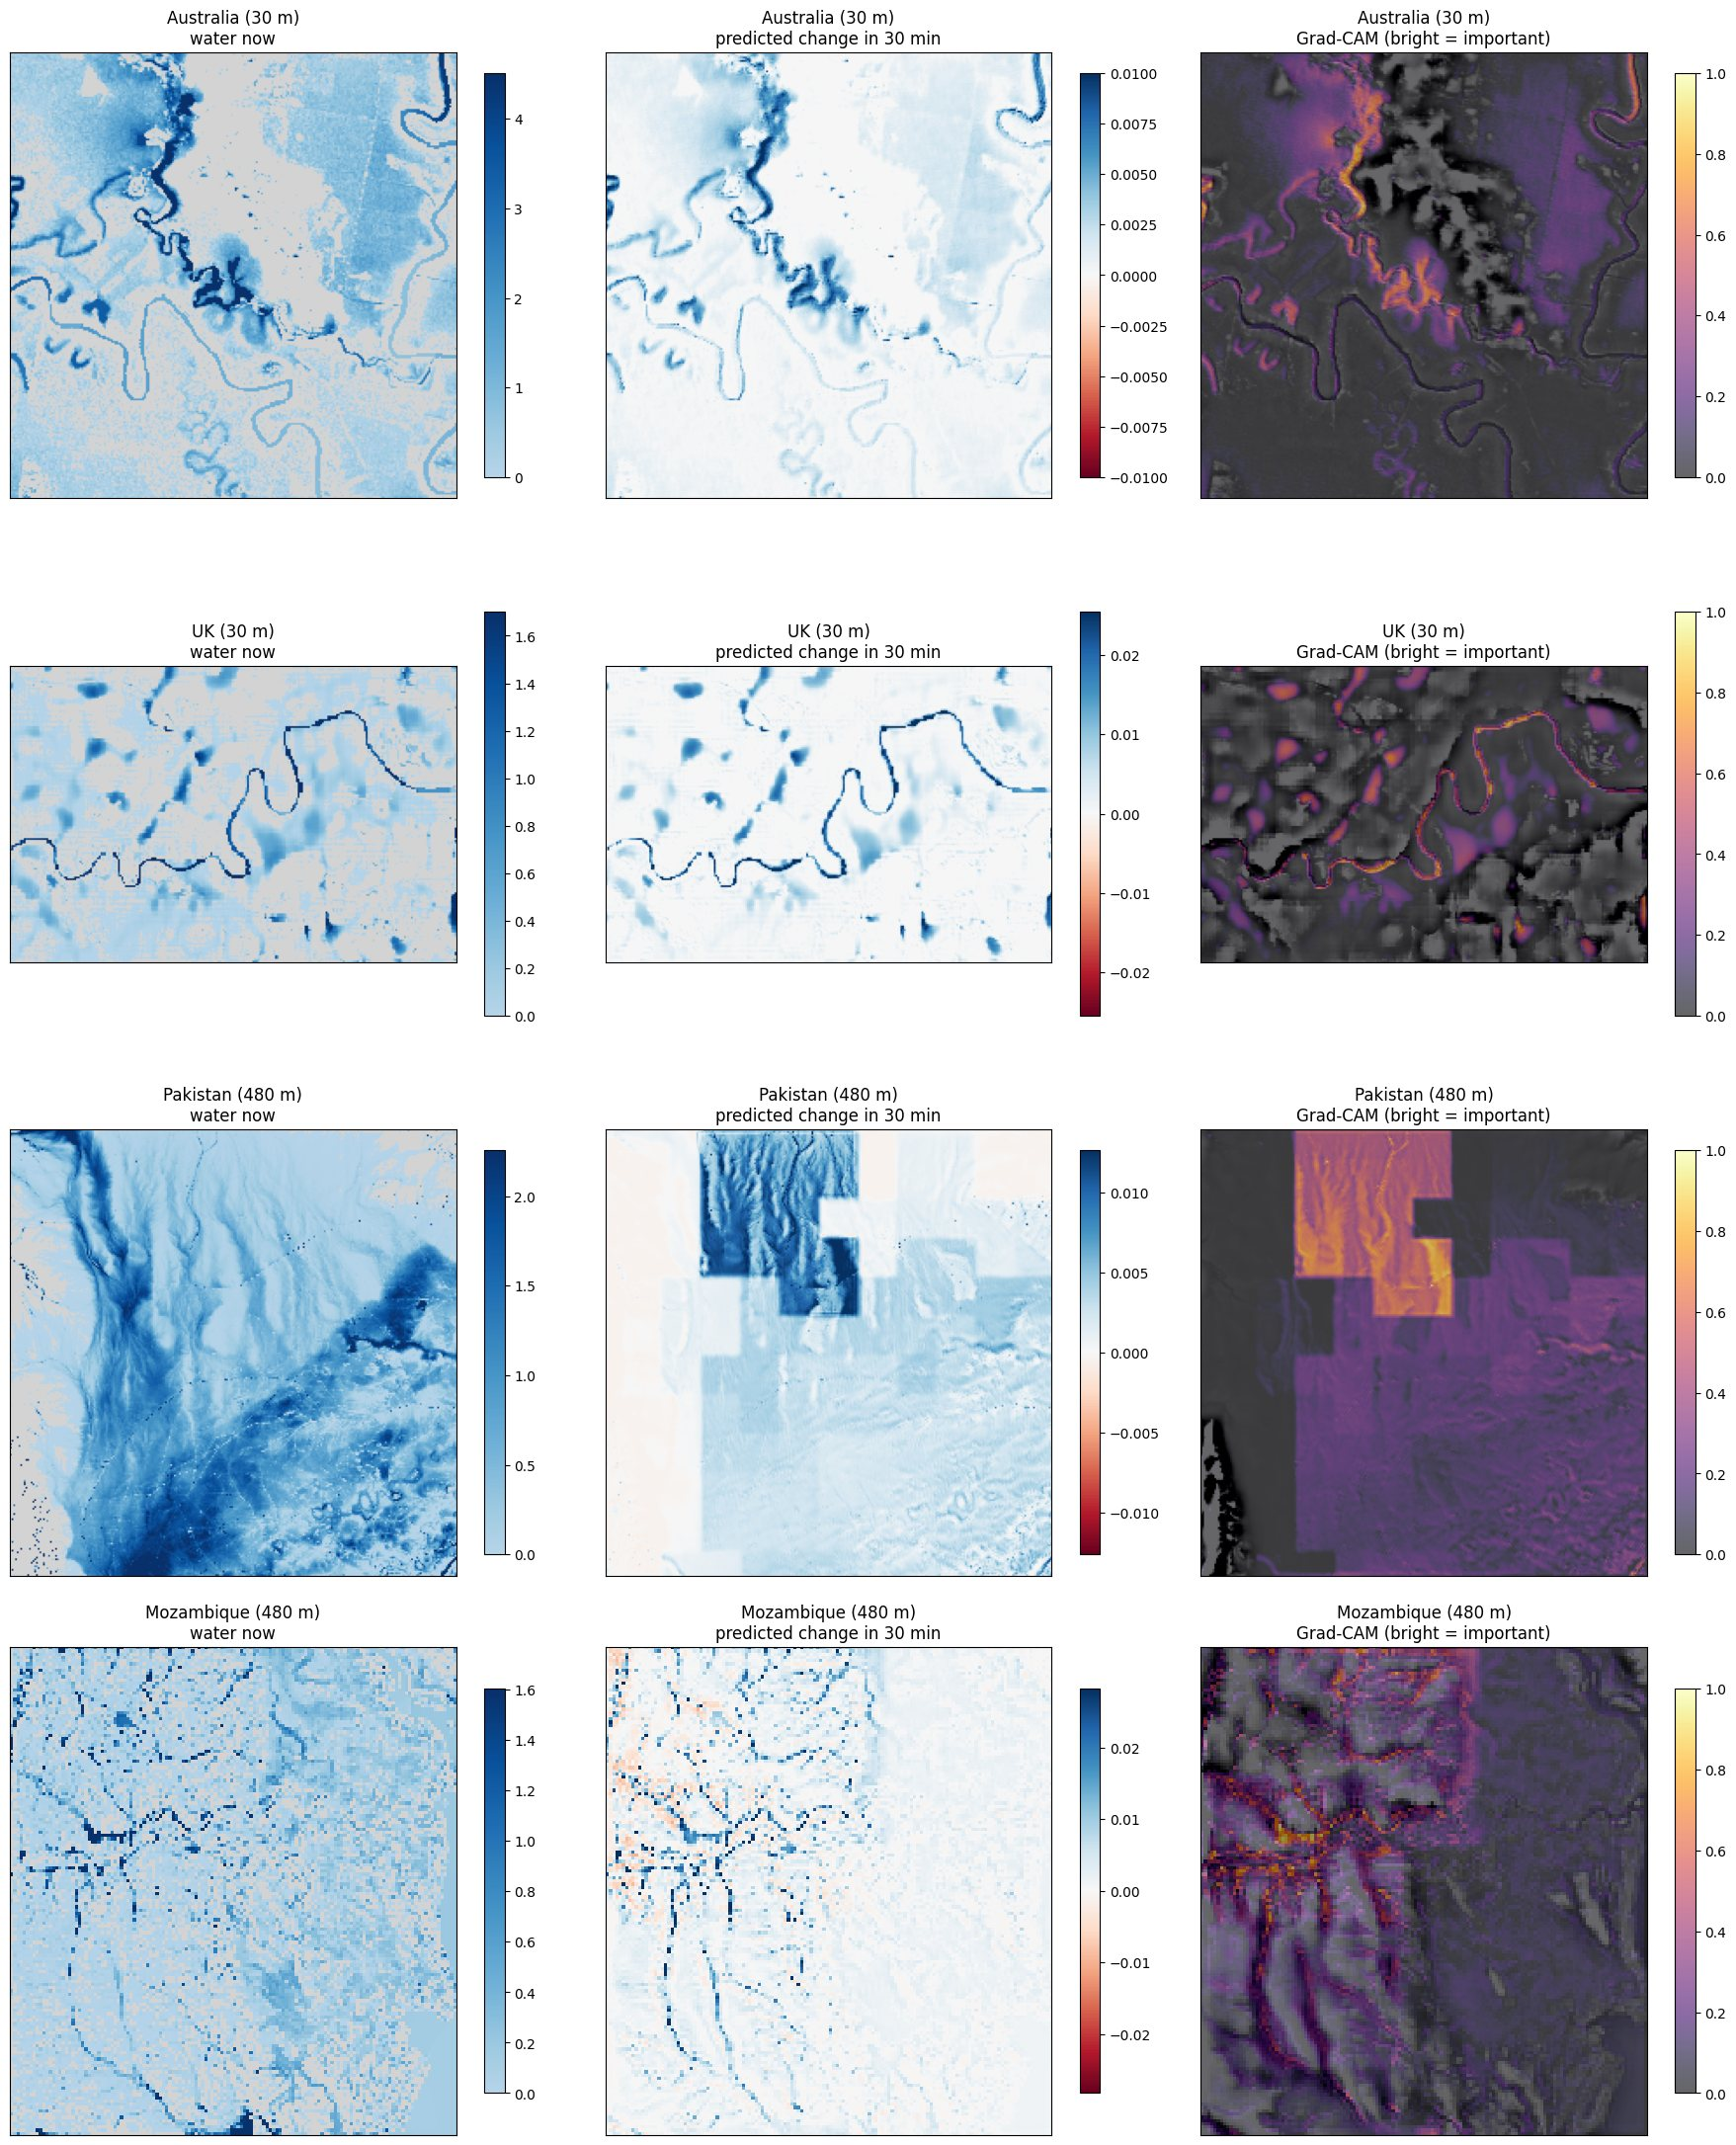
\includegraphics[width=0.4\linewidth]{nbfigs/model_c51_9.jpg}\hspace{0.01\linewidth}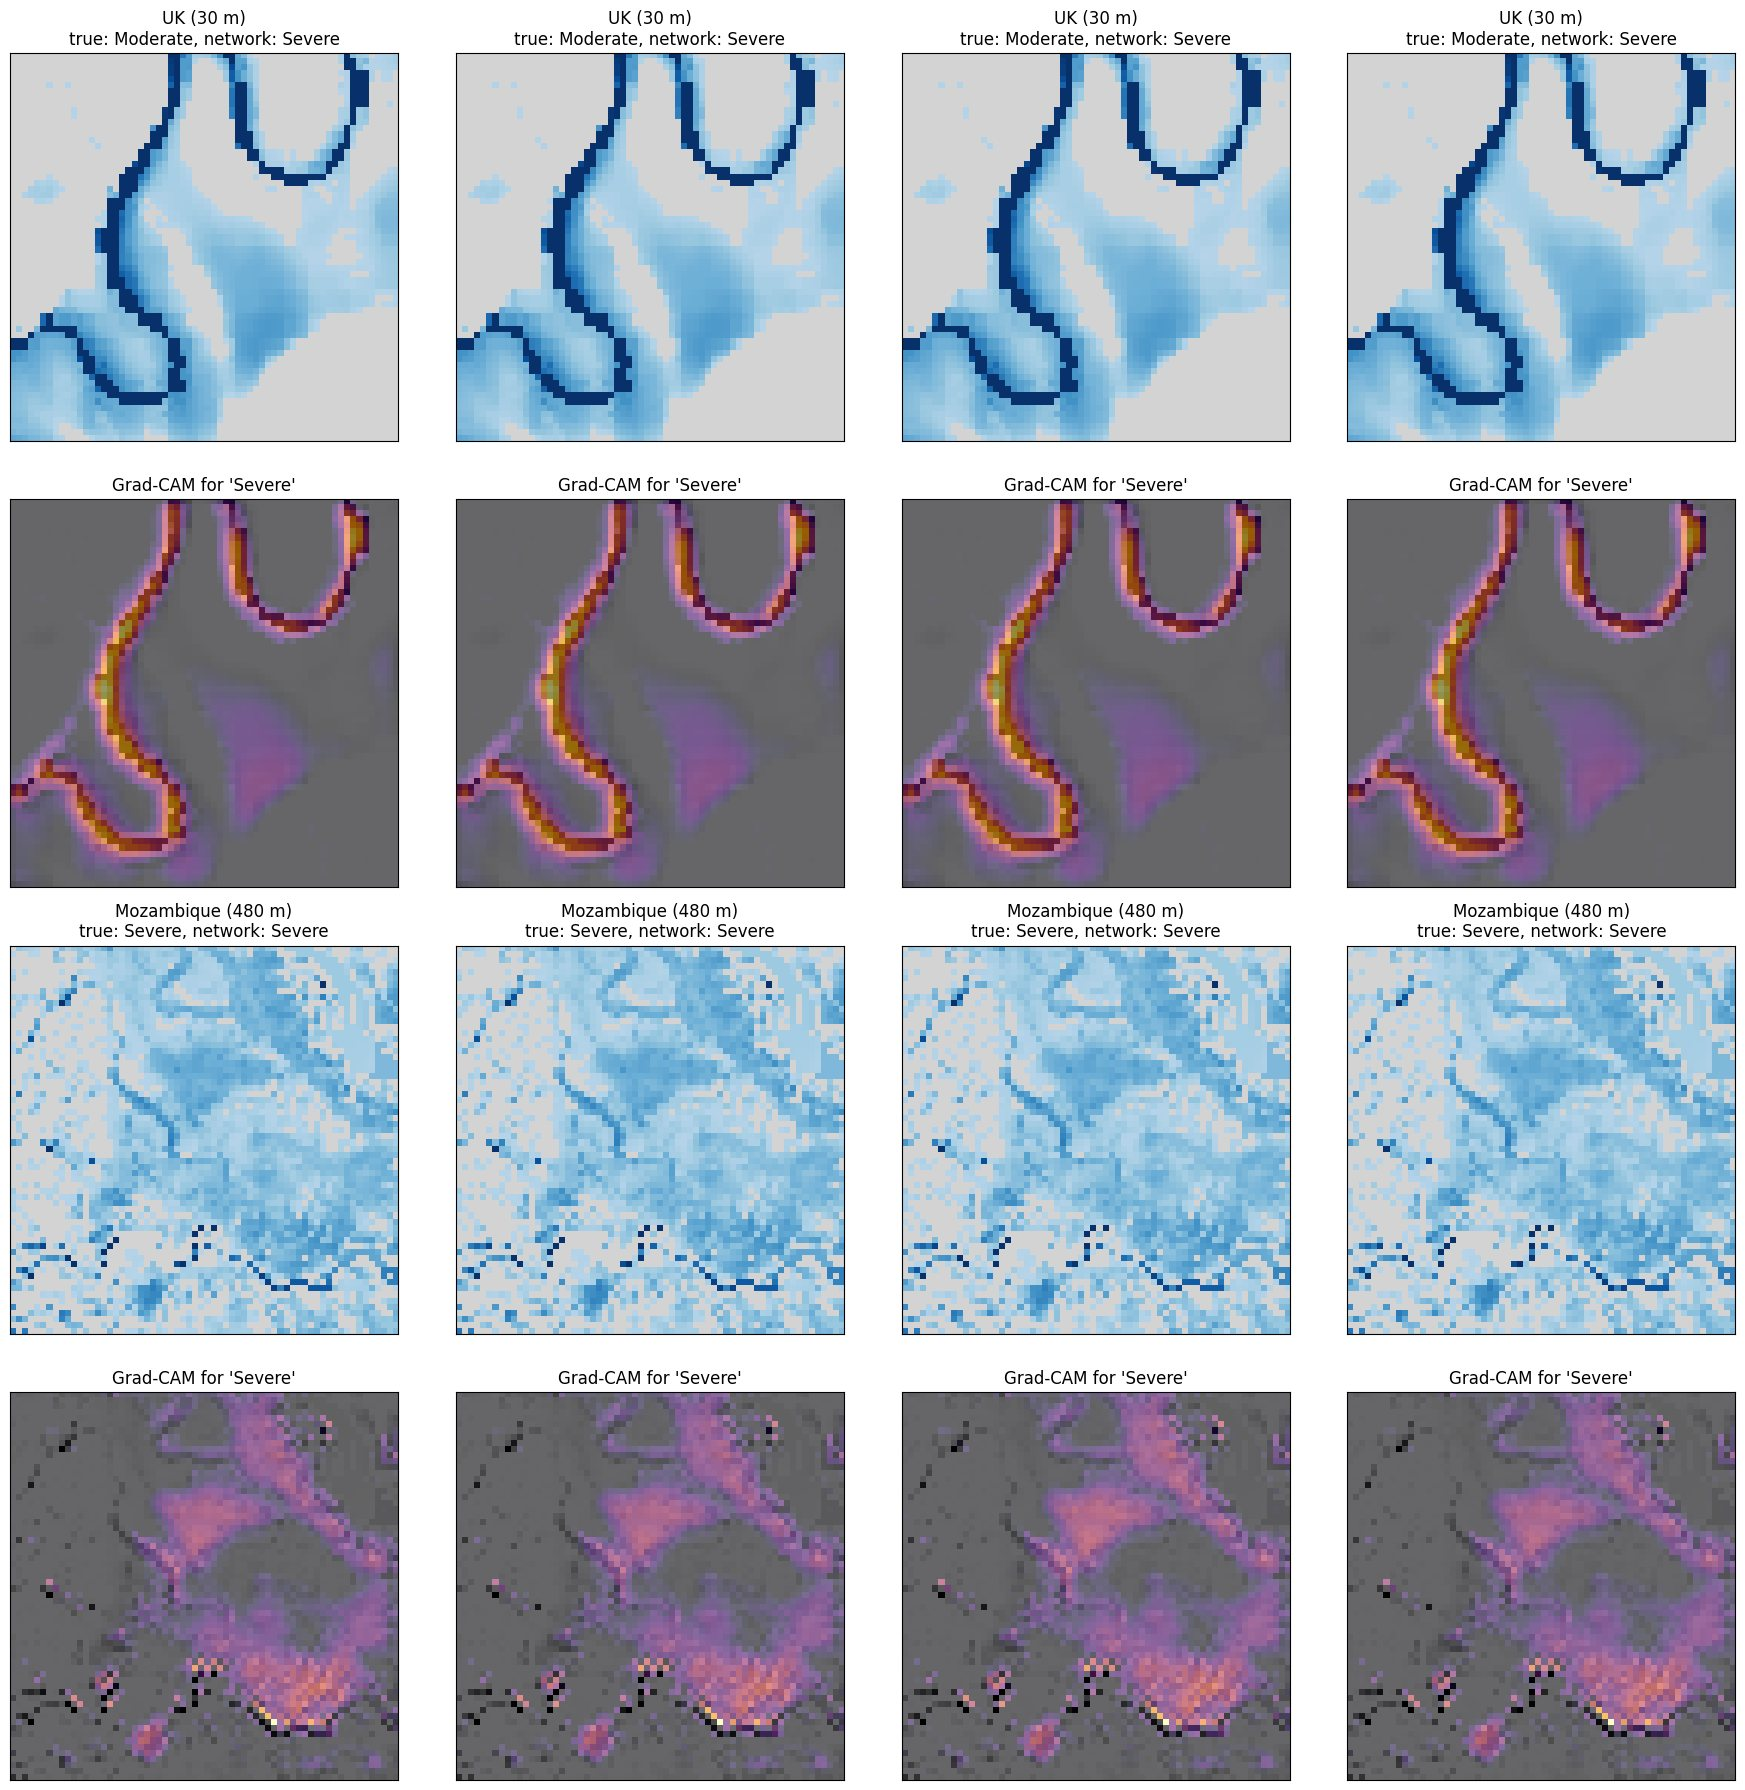
\includegraphics[width=0.3\linewidth]{nbfigs/model_c52_10.jpg}
\caption{Left: Grad-CAM of Model A (rows Australia, UK, Pakistan, Mozambique, columns water now in m, predicted change in m, heat 0 to 1). Right: capsule network (rows 1 and 2 UK, rows 3 and 4 Mozambique, water now above its heat map).}
\end{figure}
\textbf{Say this (Model A):} the heat is brightest where the predicted change is largest: the deep channel in Australia, thin lines along bends in the UK, square blocks in Pakistan (we think from blocks of heavy rain in the data, their straight edges are not how water behaves) and the drainage lines in Mozambique. It shows where the number is most sensitive, not that the forecast is right. The predicted change is tiny, about 1 to 3 cm in 30 minutes. The report adds that in the earlier laptop study deleting the top 10\% of the heat map changed the forecast more than random cells in 84\% to 92\% of windows, not run in this notebook.

\textbf{Say this (capsule):} in the UK all four tiles read ``true Moderate, network Severe'' with heat on the deep channel. In Mozambique all four read ``Severe, Severe'' with spread-out heat. The four columns look alike and are very probably one tile at neighbouring times (we think). The report says the capsule heat maps were weak (top cells beat two control sets in only 55\% of windows, two seeds agreed with rank correlation 0.17), so they are illustrations, not proof.

\qq{What number does each Grad-CAM explain, and why average gradients and use ReLU?}{Model A: the total predicted water of the window. Capsule network: the length of the chosen class capsule. Averaging gives one weight per memory map and ReLU keeps only places that push the number up, the standard recipe.}{}

% =====================================================================
\subsection{Section 7: Written rules, the NeuroSymbolic part (cells 53 to 58)}
\term{NeuroSymbolic AI} joins a network that learns patterns (Model A, capsule network) with rules people write down (these three plus the water-balance rule of Section 3a). The written reason of each decision is the explainable part.

\begin{center}
\small
\begin{tabularx}{\linewidth}{|>{\bfseries}l|Y|Y|Y|}
\hline
\rowcolor{black!12} \hd{Rule} & \hd{When it applies} & \hd{What it does} & \hd{Why (our reading)}\\ \hline
1. No water, no flood & under 1\% of dry land flooded now and in the forecast & answer None & almost nothing wet now and soon makes a higher rating implausible\\ \hline
2. Rising water & forecast flooding at least as much as now, more than 1 mm/h rain in the last hour, network class below current class & answer is the current class & flooding not shrinking during rain should not be rated below what is already there\\ \hline
3. Agree with the forecast & network more than one class from the forecast map's class & answer is the forecast map's class & the forecast map is measured from depths, the network is a guess\\ \hline
\end{tabularx}
\end{center}
The notebook gives no written reasons for the limits (1\% and 1 mm/h), so the last column is our reading.
\codelines{model_c54}{12}{25}
\cd{ALMOST\_DRY\_SHARE = 0.01} and \cd{RAIN\_RULE\_MM\_PER\_HOUR = 1.0} are the limits, and \cd{severity\_class} turns the two shares into \cd{now\_class} and \cd{forecast\_class}. Lines 12 to 14, rule 1: \cd{return 0, "Rule 1: ..."} ends the function at once. Lines 16 to 18, rule 2: three conditions joined by \cd{and}, and \cd{network\_class < now\_class} means rule 2 can only \emph{raise} the answer. Lines 20 to 23, rule 3: \cd{abs(network\_class - forecast\_class) > 1}. Line 25: no rule fired, ``No rule needed''. \textbf{Order matters}: the first rule that applies decides.

\textbf{Cell 55} runs it for every test tile. Share now and share forecast come from the last depth map and Model A's forecast tile. Rain last hour is \cd{data["inputs"][tile, -2:, :, :, 1].mean() * RAIN\_SCALE}: the last two maps (two 30-minute steps), averaged, times 10 to undo the division when the input was built, giving mm per hour.

\textbf{Cell 56} (accuracy with and without rules, saved as \cd{07\_neurosymbolic\_accuracy.csv}) and \textbf{cell 57} (which rule decided, by cutting each reason at the colon):
\begin{center}
\small
\begin{tabularx}{\linewidth}{|l|Y|Y|Y|Y|r|r|r|r|}
\hline
\rowcolor{black!12} \hd{Flood} & \hd{Capsule alone} & \hd{Forecast-map class} & \hd{Capsule + rules} & \hd{Changed} & \hd{None needed} & \hd{R1} & \hd{R2} & \hd{R3}\\ \hline
Australia (30 m) & 60.9\% & 99.8\% & 67.9\% & 7.0\% & 930 & 49 & 0 & 21\\ \hline
UK (30 m) & 50.0\% & 99.1\% & 56.1\% & 6.1\% & 939 & 0 & 40 & 21\\ \hline
Pakistan (480 m) & 87.4\% & 99.9\% & 89.1\% & 1.7\% & 983 & 0 & 7 & 10\\ \hline
Mozambique (480 m) & 63.5\% & 99.5\% & 70.7\% & 7.2\% & 824 & 134 & 42 & 0\\ \hline
\end{tabularx}
\end{center}
The gains (7.0, 6.1, 1.7, 7.2 points) equal the changed decisions (70, 61, 17, 72 tiles), and a change adds at most one correct tile, so every changed decision turned a wrong answer into a right one (our calculation). A rule that fired did not always change the answer: in Mozambique 134 tiles got rule 1 but rule 1 changed only 30 answers, in 104 the network already said None (our calculation). \textbf{Why the forecast map scores 99\%:} the rating in 30 minutes is almost the rating now because water changes slowly, so the class read off the forecast map is nearly always right (the report says the classifier adds little). Pakistan's 87.4\% is flattered by the 69.8\% baseline.

\textbf{Cell 58} shows ten example decisions (UK and Mozambique). For example UK 26.5 h, rule 3: network Severe, truth Minor, forecast map says Minor, $|3-1|=2>1$, so Minor, correct. Mozambique 76.0 h had no rule, so the mistake stays. All six changed decisions of the ten are correct, but ten rows are an illustration, not a measurement.

\qq{Did the rules help, and do they always give the right answer?}{They helped in all four floods and every changed decision became correct, but they act only when their conditions are met, so not every mistake is fixed.}{Each decision carries a reason text starting with the rule name, and cell 57 counts these names.}

% ---------------------------------------------------------------------
\subsection{Section 8: Summary and saved files (cells 59 to 61)}
\textbf{Cell 60} only copies numbers: for each flood \cd{v2\_table[v2\_table["Region"] == REGION\_NAMES[dataset]].iloc[0]} picks the Model B row, and the cell-56 accuracy row is placed beside it (saved as \cd{08\_summary.csv}).
\begin{center}
\small
\begin{tabularx}{\linewidth}{|l|l|r|r|r|Y|Y|}
\hline
\rowcolor{black!12} \hd{Flood} & \hd{Tested on} & \hd{Trend} & \hd{Model A} & \hd{Model B} & \hd{Capsule (\%)} & \hd{+ rules (\%)}\\ \hline
Australia (30 m) & unseen time & 0.990 & $-1.449$ & 0.989 & 60.9 & 67.9\\ \hline
UK (30 m) & never-seen region & 0.947 & 0.305 & 0.948 & 50.0 & 56.1\\ \hline
Pakistan (480 m) & unseen time & 0.908 & 0.345 & 0.908 & 87.4 & 89.1\\ \hline
Mozambique (480 m) & never-seen region & 0.942 & 0.150 & 0.943 & 63.5 & 70.7\\ \hline
\end{tabularx}
\end{center}
The first three numbers are skill $=1-$ (error of the forecast) / (error of copying the last map): 0 is as good as copying, 1 is perfect. Trend and Model B are close to 1 everywhere, Model A is far lower and negative in Australia, and nothing in the severity columns comes near the 99\% of the plain forecast-map class.

\textbf{Cell 61} lists what the notebook saved on Drive: 6 model files (all \cd{.weights.h5}, only loaded in this run), 24 pictures and 15 tables. This notebook writes figures \cd{02\_} to \cd{06\_} and tables \cd{01\_}, \cd{03\_}, \cd{04\_}, \cd{07\_}, \cd{08\_}. Files such as \cd{04\_capsule\_confusion.png}, \cd{05\_grad\_cam\_capsule.png}, \cd{P1} to \cd{P6} and \cd{07\_summary.csv} are written by no cell of this version. We think they are left over from earlier versions sharing the Drive folder, which is the answer if mam asks about a picture with another number. The only warning in this half is the harmless optimizer one at cell 46.

% ---------------------------------------------------------------------
\subsection{This notebook in ten lines}
\begin{enumerate}
\item \textbf{Load the data.} Four floods from Drive: Australia and UK at 30 m, Pakistan and Mozambique at 480 m. A map step is half an hour and each input has 4 maps with 3 layers (depth, rain already fallen, ground height).
\item \textbf{Cut tiles.} Models learn from 4,000 random $64\times64$ tiles (600 for checking) from the first 70\% and next 15\% in time of Australia and Pakistan, and are tested on the last 15\% of those and on the never-seen UK and Mozambique floods.
\item \textbf{Model A.} A CNN and a ConvLSTM with 62,833 parameters predict the change in depth, so next map = last map + change. Weights loaded from Drive.
\item \textbf{Results and water-balance rule.} Model A skill is 0.305, 0.345, 0.150 in the UK, Pakistan, Mozambique but $-1.449$ in Australia. The water-balance rule helps in all four.
\item \textbf{Trend forecast.} With no network, next map = last map + $\beta\times$ last change gives skill 0.990, 0.947, 0.908, 0.942 ($\beta=0.921$ at 30 m, 0.948 at 480 m).
\item \textbf{Model B.} The same network starting from the trend and learning a small correction. Skill 0.989, 0.948, 0.908, 0.943, matching the trend, not beating it.
\item \textbf{Capsule network.} It reuses the frozen CNN and ConvLSTM of Model A and rates each tile None, Minor, Moderate or Severe with 256 small capsules, 4 class capsules and the length as confidence. Right for 60.9\%, 50.0\%, 87.4\%, 63.5\% of tiles.
\item \textbf{Grad-CAM.} Heat maps show where Model A looks (channels, flood edges, rain blocks) and where the capsule network looks (weak, only pictures).
\item \textbf{Written rules.} Three severity rules plus the water-balance rule are the NeuroSymbolic part. They raise severity accuracy to 67.9\%, 56.1\%, 89.1\%, 70.7\%, with a written reason for each decision.
\item \textbf{The summary.} At 30 minutes the plain trend forecast is as good as the networks and the forecast-map class is right about 99\% of the time. A fair test of the ConvLSTM memory needs longer forecasts (6 to 24 hours), and all results are single runs on simulated floods.
\end{enumerate}
\endgroup

% =========================================================== SPEAKING SCRIPT (about 7 minutes, walks through every figure)
\section{Speaking script for the 15 slides (about 7 minutes)}\label{ch:script}

You present slides 1 to 7 (about 3 minutes 30 seconds) and Aman presents slides 8 to 15 (about 3 minutes 30 seconds). The words in quotes are what you say. The grey bracketed lines are \emph{pointing cues}: touch or point at that part of the slide while you talk. Pause for a second after each question to mam, and vary your voice. If you run late, make slides 9 and 13 one sentence each.

\newcommand{\pt}[1]{\par\noindent\hspace*{0.6em}{\small\color{black!60}\textit{[#1]}} }

\subsection{Anhad: slides 1 to 7}
\textbf{Slide 1. Title (10 s).} \pt{point at the picture} ``Hello mam, I am Anhad and this is Aman. This picture is our model on the Australia flood, and the bright lines are the rivers it watches most. Our question: can a neural network forecast a flood better than very simple rules?''

\textbf{Slide 2. The problem (35 s).} \pt{trace the four boxes, then the arrow into the network} ``When a river is about to overflow, people need to know where the water will be in the next hour. A physics simulator takes days. A network answers in seconds. We show it these four maps, 30 minutes apart, plus rain and ground height, and it draws the last box, the map 30 minutes later.'' \pt{point at the orange box} ``Here is the catch. If I say `tomorrow's weather will be like today's', I am right most days. In 30 minutes the water barely moves either, so just copying the last map is already a good forecast. The network must beat that.''

\textbf{Slide 3. The data (25 s).} \pt{sweep across the cards, then the tags} ``Four floods, re-created by a physics simulator from real terrain and satellite rain: Australia, UK, Pakistan, Mozambique. We learn from the dark-tagged ones and test on the teal-tagged ones, like studying one question paper and then getting an exam with new questions. Squares are 30 metres wide for the first pair and 480 metres for the second, so we train two separate models.''

\textbf{Slide 4. The whole system (30 s).} \pt{start at the dark Forecaster box and follow the arrows} ``The forecaster, a CNN with a ConvLSTM, predicts the next depth map. A water rule checks it against the rain, like a bathtub that can only fill as much as the tap pours in.'' \pt{drop to the bottom row} ``A capsule network rates how serious the flood is, and three written rules check that rating and give a reason, like a doctor checking a machine's report against a checklist. A network checked by rules people can read is NeuroSymbolic AI.'' \pt{red dashed arrows} ``These dashed arrows are Grad-CAM, our explainable AI.''

\textbf{Slide 5. The forecaster (35 s).} \pt{point at each box, left to right} ``In go four maps with three layers each: depth, rain and ground height. Two CNN layers pick out shapes, the way you spot a river on a satellite photo.'' \pt{dark box} ``The ConvLSTM reads the four maps in order and remembers how the water moved, like watching four frames of a video to see if it is rising. The last layers turn that memory into the predicted change in depth, not the whole map, because most of it hardly changes. The model has 62,833 parameters, the numbers on the right of the slide.''

\textbf{Slide 6. Skill, Model A and Model B (40 s).} \pt{formula} ``We score a forecast with skill: one minus its error divided by the error of copying. Zero means no better than copying, one is perfect, below zero is worse.'' \pt{red card} ``Model A learns the change from the last map. It beat copying in three of four tests, but in late Australia its skill was minus 1.449.'' \pt{teal card} ``So we built Model B. It starts from a trend forecast, the last map plus a fraction beta of the last change, like a car that keeps going at nearly the speed it just had. Beta is one number: 0.921 for 30 metres, 0.948 for 480 metres.''

\textbf{Slide 7. Main result of Part 1 (30 s).} \pt{legend, then the long blue bar} ``Orange is the trend forecast with no network, blue is Model A, green is Model B. Higher is better, and zero is copying. This blue bar is Australia, minus 1.449. Everywhere the orange bars beat the blue ones, 0.91 to 0.99 against 0.15 to 0.35.'' \pt{green bars, then 0.001} ``And the green bars match the orange to within 0.001. A rule with one number did as well as our network. Aman will explain why.''

\subsection{Aman: slides 8 to 15}
\textbf{Slide 8. Little is left to improve (25 s).} \pt{four big percentages} ``After the trend forecast, only 1 percent of copying's error is left in Australia, 5 in the UK, 9 in Pakistan, 6 in Mozambique. It is like a student who already has 95 out of 100: little left to gain.'' \pt{small charts} ``On these error charts, orange and green, trend and Model B, hug the bottom in every panel. A fair test of memory needs longer forecasts, 6 to 24 hours.''

\textbf{Slide 9. Error maps (15 s).} \pt{finger down the first column, then to the last column} ``Same story on the map, one row per flood. Left to right: the water now, what really changed, Model A's error, Model B's error. Purple is too much water, orange too little. Model B's last column is almost blank.''

\textbf{Slide 10. Part 2, the laptop study (35 s).} \pt{legend} ``Part 2 is a bigger laptop study, about 310 runs, up to 2.5 hours ahead. The three colours are three tests.'' \pt{first bars, then the lookup table} ``Our first big network scored only 0.19 and 0.06. A lookup table that uses just each square's current depth and last change already reaches 0.74 to 0.79, and a linear formula about 0.8.'' \pt{last three groups} ``The best networks reach 0.81 to 0.87, only 0.05 to 0.08 more. Like a driver who only needs the last speed: the recent history of each square gives most of the skill.''

\textbf{Slide 11. Does the memory help? (35 s).} \pt{two lines} ``Does the LSTM memory help? Skill, from 30 minutes on the left to 2.5 hours on the right. Grey is a plain CNN, teal is the ConvLSTM with memory. Both fall, because any forecast gets harder further ahead.'' \pt{the crossing} ``In this chart teal falls more slowly. But trained for the same, longer length, 90 passes, they scored the same: plus 0.004 and minus 0.014, inside our plus or minus 0.03 band. A model 140 times bigger did no better.''

\textbf{Slide 12. Severity and written rules (30 s).} \pt{small tables} ``The capsule network rates each tile none, minor, moderate or severe, like flood warnings from green to red. In these tables the dark diagonal is correct answers.'' \pt{bottom bars} ``Grey is the capsule network alone, teal is with our three rules: the rules raised accuracy in all four floods, for example 60.9 to 67.9 percent in Australia. The dark bars show the rating read straight from the forecast map is right about 99 percent of the time, because severity in 30 minutes is almost the same as now.''

\textbf{Slide 13. Grad-CAM (25 s).} \pt{left block, then right block} ``Grad-CAM is a highlighter showing which parts of the input the model used. On the left, the forecaster: the bright areas follow the river channels and flood edges, where the water is changing. On the right, the capsule network on the UK and Mozambique: those heat maps were weak, so we show them as pictures, not proof.''

\textbf{Slide 14. What we learned (35 s).} \pt{numbers 1, 2, 3} ``One: at 30 minutes a trend with one number does most of the work, and our second model matches it but does not beat it. Two: up to 2.5 hours a lookup table scores 0.74 to 0.79, the best networks 0.81 to 0.87, and memory did not help at equal training. Three: always compare a model with simple forecasts. Our first model looked good until we did.'' \pt{boxes below} ``Limits: one flood per region, simulated data, single runs. Next: 6 to 24 hours ahead, where the memory could matter.''

\textbf{Slide 15. Thank you (5 s).} \pt{look at mam} ``Thank you, mam. We are happy to take your questions.''

\begin{carefulbox}
If the linear-model bars on slide 10 still show 0.32, 0.35 and 0.15, say: ``Those linear bars are from our first fit, which had a bug. After the fix it scores 0.82, 0.80 and 0.79, so the conclusion does not change.''
\end{carefulbox}

% =========================================================== WHO DID WHAT (short)
\section{Who did what, and where to find everything}\label{ch:who}
\textbf{Aman Sumeet Saxena} built and ran the Colab work (Part 1) and wrote the three final notebooks (Data exploration, Data preparation, Flood model): data checks, Models A and B, trend forecast, water-balance rule, capsule network, severity rules, Grad-CAM. \textbf{Anhad Mahajan} ran the laptop study (Part 2, about 310 training runs), the baselines, ablations, strict tests and the earlier capsule and Grad-CAM tests. The report is joint. Aman found the ridge baseline mistake (Chapter~\ref{ch:bug}) and the baselines were re-fitted with rescaled inputs, with the original code file left unchanged.

\begin{table}[!htbp]
\centering\footnotesize
\caption{Where things are.}
\begin{tabularx}{\linewidth}{|>{\bfseries}p{3.6cm}|Y|}
\hline
Final report (Word, PDF) & The 28-page report we hand in, the source of the results in this guide.\\ \hline
Final presentation & The 15-slide deck, with the script in Chapter~\ref{ch:script}.\\ \hline
Three Colab notebooks & Already run, outputs saved (Chapters~\ref{ch:nb-explore}, \ref{ch:nb-prep}, \ref{ch:nb-model}).\\ \hline
Laptop study package & The Part 2 code, the roughly 310 result files and the project log.\\ \hline
Ridge baseline check & Scripts, notes and an erratum for the fix of Chapter~\ref{ch:bug}.\\ \hline
Website and README & https://amans-06.github.io/FloodCastBench-Project/ and the GitHub repository FloodCastBench-Project.\\ \hline
\end{tabularx}
\end{table}

\textbf{Running the notebooks (in this order, outputs are already saved, so for the talk just scroll).} (1) \emph{Data exploration} needs about 30 GB of free disk (Colab showed 62.9 GB), downloads all 14,870 files (about 27 GB, 60 minutes in our run) and saves nothing to Drive. (2) \emph{Data preparation} downloads only 3,822 files (9.1 minutes), writes 5.69 GB of arrays to Colab's disk and compares them with the copy on Drive, which it only reads. (3) \emph{Flood model} needs a T4 GPU runtime and loads the prepared data and saved models from Drive. \cd{TRAIN\_NEW} and \cd{TRAIN\_V2} are False, so nothing is trained again, and True trains again.

\section{A to Z of new words}\label{ch:gloss}
\begin{multicols}{3}
\scriptsize
\setlength{\parskip}{0.05em}
\raggedright
\textbf{Ablation.} Removing one input or part to see how much the score falls.\par
\textbf{Adam.} A method that adjusts the learning step during training.\par
\textbf{Array.} A grid of numbers in numpy, with a shape.\par
\textbf{Augmentation.} Extra training examples made by rotating and flipping.\par
\textbf{Baseline.} A simple forecast a model must beat.\par
\textbf{Batch.} Examples looked at before each weight nudge.\par
\textbf{Capsule.} A unit giving a short list of numbers, whose length says how sure it is.\par
\textbf{Capsule network.} Capsules that vote for each other (routing by agreement).\par
\textbf{Causal rain.} Only rain that has already fallen.\par
\textbf{Cell.} One box of a Colab notebook, code or writing.\par
\textbf{Channel.} One layer of a map (depth, rain, height).\par
\textbf{CNN.} Convolutional network, slides small filters over a map.\par
\textbf{Colab.} Free online notebook that lends a GPU.\par
\textbf{Confusion matrix.} Table of right and wrong answers of a classifier.\par
\textbf{ConvLSTM.} An LSTM whose memory is a map and whose gates use filters.\par
\textbf{Copy forecast.} Next map equals last map (persistence).\par
\textbf{CPU and GPU.} Normal processor and graphics chip, the GPU is much faster for networks.\par
\textbf{DataFrame.} A pandas table with named columns.\par
\textbf{Deletion test.} Removing the hottest heat-map cells to see if the forecast changes more than for random cells.\par
\textbf{Dense layer.} Every neuron sees every number of the layer before.\par
\textbf{E60, E30, E480.} Part 2 experiments: Australia to UK at 60 m and 30 m, Pakistan to Mozambique at 480 m.\par
\textbf{Early stopping.} Stop when the mock-test score stops improving.\par
\textbf{Epoch.} One pass through all training examples.\par
\textbf{Explainable AI.} Tools that show what a model is doing.\par
\textbf{FABDEM.} Ground height map used by the simulator.\par
\textbf{Filter.} Small window of weights sliding over a map.\par
\textbf{FloodCastBench.} Public dataset of four simulated floods.\par
\textbf{Fold.} One of three rounds with a different third of tiles held out.\par
\textbf{Forced rain.} The next five rain maps are given too.\par
\textbf{Frozen.} Weights not changed in training.\par
\textbf{GPM-IMERG.} Satellite rain data used by the simulator.\par
\textbf{Grad-CAM.} Heat map of which places mattered for an answer.\par
\textbf{Gradient.} Slope telling which way to change a weight to lower the loss.\par
\textbf{Grid.} A map made of squares holding numbers.\par
\textbf{Hugging Face.} Website that stores datasets and models.\par
\textbf{Hybrid rain.} The original input, with up to 30 minutes of rain not yet fallen.\par
\textbf{Hypothesis.} A guess we test, written down before the final runs.\par
\textbf{Keras, TensorFlow.} Free libraries for building networks.\par
\textbf{Kernel.} Another word for filter.\par
\textbf{Label.} The right answer used to train a classifier.\par
\textbf{Learning rate.} Size of each weight step.\par
\textbf{Linear model.} A weighted sum of inputs.\par
\textbf{Lookup table.} Average answer looked up for each pair of values.\par
\textbf{Loss.} How wrong the network is, learning makes it small.\par
\textbf{LSTM.} Long short-term memory, with forget, write and read gates.\par
\textbf{Margin loss.} Capsule loss: correct capsule above 0.9, others below 0.1.\par
\textbf{Mean squared error.} Average of squared mistakes.\par
\textbf{MLP.} Multilayer perceptron, small network of dense layers.\par
\textbf{Model A, Model B.} Part 1 forecasters, A starts from the last map, B from the trend.\par
\textbf{Neural network.} Many simple neurons with learned weights.\par
\textbf{NeuroSymbolic AI.} A network checked by written rules.\par
\textbf{Never-seen flood.} Flood hidden during training (UK, Mozambique).\par
\textbf{Notebook.} Colab file of cells, outputs stay saved.\par
\textbf{NPY file.} One saved numpy array.\par
\textbf{Overfitting.} Memorising practice examples and failing on new ones.\par
\textbf{Parameter.} A number the network learns, such as a weight.\par
\textbf{Pass.} One run through all training examples.\par
\textbf{Pixel.} One square of a picture or map.\par
\textbf{Rank correlation.} How alike two maps order places, 1 same, near 0 none.\par
\textbf{Rasterio.} Library that reads map files (tif) into arrays.\par
\textbf{ReLU.} Turns negative numbers into zero.\par
\textbf{Ridge regression.} Linear fit with a penalty keeping weights small.\par
\textbf{RMSE.} Root mean square error, typical mistake in the original unit.\par
\textbf{Routing by agreement.} Capsules whose votes agree get more weight.\par
\textbf{Seed.} Number that fixes the random start so a run repeats.\par
\textbf{Shape.} Size of an array in each direction, e.g. 4, 64, 64, 3.\par
\textbf{Skill.} 1 minus forecast error divided by copy error.\par
\textbf{Spatiotemporal.} In both space and time.\par
\textbf{Squash.} Shrinks a vector to length 0 to 1, keeping its direction.\par
\textbf{Strict split.} Test where a block of time is also hidden from training.\par
\textbf{Tile or patch.} Small square cut from a big map.\par
\textbf{Token.} Secret key (Hugging Face) kept in Colab secrets.\par
\textbf{Training, validation, test.} Practice questions, mock test, final exam.\par
\textbf{TRAIN\_NEW.} Model notebook switch: False loads saved models, True trains again.\par
\textbf{Trend forecast.} Last map plus a fraction of the last 30-minute change.\par
\textbf{Water-balance rule.} Shifts a forecast so its total rise matches the rain.\par
\textbf{Weight.} Number a neuron multiplies an input by.\par
\textbf{Window.} Part 2 example: a 128 by 128 patch with its maps in time.\par
\end{multicols}

% =========================================================== ONE-LINE ANSWERS (last chapter)
\section{One-line answers to the questions mam may ask}\label{ch:viva}\label{ch:oneliners}

Say the bold line. The small print is only for when she asks for more. Questions about each layer and number of the model (why 16 filters, why a second convolution) are in Chapter~\ref{ch:design}.

\subsection{The project and the data}
\qq{What is your project about?}{We forecast flood depth maps 30 minutes ahead with a CNN-LSTM and test whether it beats very simple forecasts like copying the last map.}{Input: the last four maps plus rain that has already fallen plus ground height. Tested on floods the model never saw.}
\qq{Why this dataset?}{FloodCastBench gives the water depth every 5 minutes for four floods in four countries at several map sizes, with rain and ground height, so we always know the right answer.}{Its own benchmark has U-Net and FNO but no recurrent model and no simple-forecast comparison.}
\qq{Is the data real?}{It is simulated from real terrain, land cover and satellite rain, so our models learn to imitate the simulator.}{We say this on the limits slide.}
\qq{What is the novelty?}{A careful test of a convolutional-recurrent model on FloodCastBench against simple forecasts on never-seen floods, plus one pipeline with written rules and heat maps.}{We did not invent a new architecture.}
\qq{What is your result in one line?}{A trend forecast with one fitted number scores 0.91 to 0.99 at 30 minutes, matching our network, so always compare a model with simple forecasts.}{Model A scored 0.15 to 0.35 and $-1.449$ in late Australia. Model B matches the trend.}
\qq{Is it useful in real life?}{Not yet as a warning system, but it is a fair test of whether such a network is worth using, and it answers in seconds while the simulator takes days.}{}
\qq{Why CNN-LSTM?}{The CNN sees neighbouring squares and the LSTM remembers how the water has been moving, and it was the model in our project title.}{}
\qq{Why only 30 minutes ahead?}{Rain maps come every 30 minutes, so it is the natural step and the simplest fair test, and longer forecasts are our next step.}{The laptop study went up to 2.5 hours.}
\qq{Why train on Australia and Pakistan, test on UK and Mozambique?}{The test is a flood in another country that the model never saw, and the 30 m and 480 m maps need separate models.}{}
\qq{Why a 70, 15, 15 split?}{The first 70\% of a flood trains, the next 15\% decides when to stop, the last 15\% tests, and splitting in time makes the test part truly later.}{}
\qq{Is there data leakage?}{No, beta is fitted only on the training part, early stopping uses only the checking part, and the tests use unseen time and unseen floods.}{In the notebook we did not choose a setting by looking at test scores.}

\subsection{Score, trend forecast and models}
\qq{What is skill?}{One minus the error of the forecast divided by the error of copying the last map, so 0 is the same as copying, 1 is perfect, below 0 is worse.}{Accuracy does not suit depth maps, which hold a number in every square.}
\qq{What is CSI?}{Of the squares flooded (above 30 cm) in the forecast or in reality, the share where both agree.}{}
\qq{What is the trend forecast?}{The last map plus beta times the last change, never below zero, with no network, and beta is 0.921 for 30 m and 0.948 for 480 m.}{}
\qq{Model A against Model B?}{Same layers, 62,833 parameters, but A starts from the last map and B starts from the trend and learns only a small correction.}{}
\qq{Why did you build Model B?}{The trend forecast beat Model A by a lot, so we asked whether a network that starts from the trend could improve on it.}{}
\qq{Why does Model B only match the trend?}{At 30 minutes only 1, 5, 9 and 6\% of copying's error is left after the trend, so there is almost nothing to add.}{A fair test of the memory needs 6 to 24 hours.}
\qq{Why is Model A negative in Australia?}{In the last part of that flood the water hardly moves and copying is off by about a millimetre, while Model A adds a little water almost everywhere.}{We first thought it never saw draining water, but 73 of 331 training steps had falling water.}
\qq{Skill numbers?}{Trend 0.990, 0.947, 0.908, 0.942, Model A $-1.449$, 0.305, 0.345, 0.150, Model B 0.989, 0.948, 0.908, 0.943.}{Order: Australia last 15\%, UK, Pakistan last 15\%, Mozambique.}
\qq{What did the 310-run laptop study show?}{Up to 2.5 hours the depth history carries almost all the skill: lookup table 0.74 to 0.79, best networks 0.81 to 0.87.}{}
\qq{Does the LSTM memory help?}{Not at equal training length: the difference is $+0.004$ on the UK and $-0.014$ on Mozambique, inside our $\pm0.03$ band.}{With the 30-pass training it lost less skill at longer lead times and stayed stable when the flood start was hidden. We did not test why.}
\qq{What did the ridge mistake do?}{It made the linear baseline score 0.15 to 0.36 instead of 0.79 to 0.82, and Aman found and fixed it.}{Slide 10 shows the corrected numbers.}

\subsection{NeuroSymbolic AI, capsule network, Grad-CAM}
\qq{What is NeuroSymbolic AI and what did you do?}{A neural network checked by written rules people can read: the water-balance rule plus three severity rules, each with a written reason.}{Rule 1: under 1\% flooded now and forecast means None. Rule 2: the class cannot fall below the current one if the forecast is not less flooded and over 1 mm per hour of rain fell in the last hour. Rule 3: if network and forecast map differ by more than one class, the forecast map wins.}
\qq{What is the water-balance rule?}{It shifts the forecast so the total rise of the water matches the rain of the last 30 minutes times 0.5 hours.}{It halved the Australian failure ($-1.449$ to $-0.710$) but adds nothing to Model B. The law holds closely, ratios 0.999, 0.946, 1.028, 1.045.}
\qq{Where is Grad-CAM?}{In the flood model notebook, Section 6, the function \cd{grad\_cam}, shown for the forecaster and for the capsule network.}{}
\qq{What is Grad-CAM?}{A heat map of which places mattered most for an answer, from the gradient of one number with respect to the ConvLSTM memory maps.}{Bright follows rivers and flood edges. The capsule heat maps were weak, so they are pictures, not proof.}
\qq{What is a capsule network?}{A network whose units give a short vector whose length tells how sure it is, with votes combined by routing by agreement.}{}
\qq{Did the capsule network work?}{Partly: 60.9, 50.0, 87.4, 63.5\% and with the rules 67.9, 56.1, 89.1, 70.7\%, but the forecast map's own class is right about 99\%.}{It did not beat a plain layer once we used augmentation.}
\qq{Is Pakistan's 87.4\% great?}{No, 698 of the 1,000 test tiles are severe, so always answering severe is right 69.8\% of the time.}{}

\subsection{Why not, and what next}
\qq{Why not real flood data?}{Real depth maps every few minutes over a region do not exist, since satellites pass every few days, so a simulator gives the complete maps.}{}
\qq{Why not 6 to 24 hours?}{It needs forecasts fed back as input and an assumption about future rain, so it is our main next step.}{}
\qq{Why not more floods or seeds?}{FloodCastBench has only four floods, so only two independent train and test pairs, and the Colab results are single runs.}{}
\qq{Why not tune more?}{Differences below about 0.02 were inside seed noise in the laptop study, so tuning could not change the conclusion.}{}
\qq{Next steps?}{Forecast 6 to 24 hours ahead, rebuild the capsule network and Grad-CAM on Model B, and repeat with several seeds.}{}

\subsection{The work and the notebooks}
\qq{What problems did you face?}{A one-hour 27 GB download with rate limits, aligning the layers, our first model failing against the trend, big maps in Grad-CAM, a bad severity label and the ridge mistake.}{}
\qq{Why three notebooks?}{Downloading and exploring, preparing, and modelling are three big slow jobs, and the prepared data is saved so each can start from files.}{}
\qq{Did the notebook train the models?}{No, it loads the saved models from Drive, and setting \cd{TRAIN\_NEW} to True trains them again with the \cd{fit} cell.}{The notebook does not show the training time. Training stops early, after at most 20 epochs.}
\qq{Who did what?}{Aman built and ran the Colab notebooks, Anhad ran the laptop study, both wrote the report, and Aman found the ridge mistake.}{}
\qq{How do you know the data preparation is right?}{Every file arrived, every layer covers the depth map, two independent alignment tests agree, and all 30 saved files are identical to the copy on Drive.}{}
\qq{Why is your model worse than a trivial baseline, and why present it?}{That is the finding: beating copying looked like success until we compared with the trend, and showing it is more useful than hiding it.}{}
\qq{Where is the code for the 310 runs?}{It was a separate 20-hour run on a laptop, its results are on slides 10 and 11, and the code we show you is in the three Colab notebooks.}{}
\qq{Why trust a simulator?}{We do not take it as truth, it follows basic water-flow rules with real ground and rain and is published, and our models only imitate it.}{}

\subsection{Reading the code}
\qq{What does None mean in (None, 4, 64, 64, 3)?}{It is the batch size, which can be any number, and the rest is one example: 4 maps of 64 by 64 with 3 layers.}{}
\qq{What does inputs[:, -1, :, :, 0:1] select?}{The depth layer of the newest map for every example, keeping the layer axis.}{All batch items, last map in time, all rows and columns, first layer only.}
\qq{What does [None] do?}{It adds a batch axis of length 1, so one map (4, H, W, 3) becomes (1, 4, H, W, 3).}{}
\qq{What does model(x, training=False).numpy()[0, :, :, 0] do?}{It runs the model in prediction mode and takes the one example and its one layer, leaving a 2D depth map.}{}
\qq{What does set\_random\_seed(42) do?}{It fixes the random numbers so a rerun gives the same result.}{}
\qq{What do np.load and np.save do?}{They read an array from a file and save one to a file, and \cd{mmap\_mode="r"} reads a big file piece by piece.}{}
\qq{What do glob.glob and [::6] do?}{\cd{glob.glob} lists files matching a pattern, and \cd{[::6]} keeps every sixth item, one map every 30 minutes from every 5.}{}
\qq{What does uniform\_filter(size=15) do?}{It replaces each square by the average of the 15 by 15 squares around it, used to get the local ground height.}{}
\qq{What does np.stack do?}{It puts arrays on top of each other along a new axis, here depth, rain and height as 3 layers.}{}
\qq{What do compile, fit and predict do?}{Compile chooses optimiser and loss, fit trains on the training tiles, predict runs the trained network on new inputs.}{}
\qq{What does set\_weights(get\_weights()) do?}{It copies the learned numbers into a model with the same layers, for example one the size of a whole map.}{}
\qq{What does tf.GradientTape do?}{It records the calculation so we can find gradients, which Grad-CAM needs.}{}
\qq{What does np.digitize do?}{It turns a flooded share into a severity class from 0 to 3 using the limits 5, 15, 30\%.}{}
\qq{What does confusion\_matrix do?}{It counts how many tiles of each true class got each answer, and the diagonal is correct.}{}
\qq{What are the harmless warnings?}{\cd{NotGeoreferencedWarning} means the map file has no position inside it, the HTTP 429 lines mean the server asked us to slow down, and the Adam warning means the saved optimiser memory is skipped.}{}

\end{document}
